% Nafs-Aql technical report (IEEEtran journal style). Build: ../../tools/tectonic nafs_aql_report.tex
\documentclass[journal]{IEEEtran}
\usepackage[utf8]{inputenc}
\usepackage[T1]{fontenc}
\usepackage{amsmath,amssymb,amsthm}
\usepackage{booktabs,array,multirow}
\usepackage{graphicx,xcolor}
\usepackage{tikz,pgfplots}
\pgfplotsset{compat=1.18}
\usetikzlibrary{arrows.meta,positioning,shapes.geometric,fit,calc,backgrounds}
\usepackage{enumitem}
\setlist{nosep,leftmargin=*}
\usepackage{listings}
\usepackage{microtype}
\usepackage{url}
\usepackage[hidelinks,pdfauthor={Dirac R\&D Team}]{hyperref}
\usepackage{cite}
% Shared palette, TikZ styles and macros for all Nafs-Aql documents
\definecolor{navy}{HTML}{1F3A5F}
\definecolor{teal}{HTML}{1B8A8F}
\definecolor{amber}{HTML}{C97D10}
\definecolor{crimson}{HTML}{B3263E}
\definecolor{violet}{HTML}{6A4C9C}
\definecolor{leaf}{HTML}{3A8F4B}
\definecolor{slate}{HTML}{5B6770}
\definecolor{sand}{HTML}{F4EFE6}
\tikzset{
  blk/.style={rounded corners=2.5pt,draw=#1!85!black,fill=#1!12,thick,align=center,
              font=\scriptsize,inner sep=3pt,minimum height=0.72cm},
  blk/.default=navy,
  sblk/.style={rounded corners=2.5pt,draw=#1!85!black,fill=#1!12,thick,align=center,
              font=\tiny,inner sep=2pt,minimum height=0.55cm},
  sblk/.default=navy,
  dm/.style={diamond,aspect=2.2,draw=amber!85!black,fill=amber!15,thick,font=\tiny,
             align=center,inner sep=0.5pt},
  st/.style={circle,draw=#1!85!black,fill=#1!15,thick,font=\scriptsize,minimum size=0.78cm,inner sep=0pt},
  st/.default=navy,
  arr/.style={-{Stealth[length=4pt,width=3pt]},thick,draw=slate},
  dsh/.style={-{Stealth[length=4pt,width=3pt]},thick,dashed,draw=slate!80},
  lab/.style={font=\tiny,fill=white,inner sep=1pt,text=black!80},
  grp/.style={rounded corners=4pt,draw=#1!60,dashed,thick,inner sep=5pt,fill=#1!4},
  grp/.default=slate,
  grplab/.style={font=\tiny\bfseries,text=#1!80!black,anchor=north west,inner sep=2pt},
  grplab/.default=slate
}
\pgfplotsset{every axis/.append style={font=\scriptsize,grid=major,grid style={black!10},
  legend style={font=\tiny,draw=none,fill=white,fill opacity=.85,text opacity=1},
  tick label style={font=\tiny},label style={font=\scriptsize}}}
% ---- shared names (single source of truth) ----
\newcommand{\Sys}{Nafs-Aql}
\newcommand{\Sone}{System~1}
\newcommand{\Stwo}{System~2}
\newcommand{\Gate}{Aql Gate}
\newcommand{\Hub}{Verifier Hub}
\newcommand{\Ledger}{Muhasaba Ledger}
\newcommand{\Distil}{Tazkiya Distillation}
\newcommand{\Mem}{Context Manager}
\newcommand{\Gw}{Rust Gateway}
\newcommand{\Harness}{Eval Harness}

\newcommand{\MEASUREDROWS}{Qwen3-4B Q4\_K\_M & 2.32\,GiB & $38.2\pm0.6$ & $6.7\pm0.8$ \\ Qwen3-4B-Thinking-2507 Q4\_K\_M & 2.32\,GiB & $38.4\pm1.5$ & $7.0\pm0.9$ \\}
\newcommand{\NREQ}{99}
% Generated by scripts/gen_publication.py; do not edit.
\newcommand{\PhaseTwoRun}{\texttt{7ffd4442}}
\newcommand{\PhaseTwoTable}{\begin{tabular}{lrrrrr}\toprule System & $n$ & Acc. & 95\% CI & Esc. & Wall (s)\\\midrule fast\_only & 6 & 67\% & [22\%, 96\%] & 0\% & 13 \\
nafs\_aql & 6 & 100\% & [54\%, 100\%] & 33\% & 96 \\
nafs\_blind & 6 & 67\% & [22\%, 96\%] & 17\% & 133 \\
slow\_conditioned & 6 & 100\% & [54\%, 100\%] & 100\% & 319 \\
slow\_only & 6 & 100\% & [54\%, 100\%] & 100\% & 264 \\ \bottomrule\end{tabular}}
\newcommand{\BlindRouting}{50\%}
\newcommand{\GatedCostRatio}{0.36}
\newcommand{\VerifierTable}{\begin{tabular}{lrrrrr}\toprule Verifier & Correct & $r$ & Mutants & $\varphi$ & $\varphi$ upper \\\midrule code\_tests & 364 & 0.995 & 754 & 0.109 & 0.133 \\
json\_schema & 24 & 1.000 & 53 & 0.000 & 0.067 \\
judge & 23 & 1.000 & 22 & 0.045 & 0.228 \\
math\_numeric & 2000 & 1.000 & 2800 & 0.000 & 0.001 \\ \bottomrule\end{tabular}}
\newcommand{\RatesRuns}{\texttt{de66e962}, \texttt{f7991b65}, \texttt{50ff0d27}, \texttt{fd07e0a8}, \texttt{dc7168b0}}
\newcommand{\ProtocolRun}{\texttt{6c462074}}
\newcommand{\ProtocolTable}{\begin{tabular}{rrrrr}\toprule Sessions & p50 (s) & p95 (s) & p99 (s) & req/s\\\midrule 1 & 3.8 & 7.2 & 7.2 & 0.25 \\
2 & 2.7 & 4.9 & 7.2 & 0.68 \\
4 & 3.6 & 9.0 & 12.0 & 0.76 \\ \bottomrule\end{tabular}}
\newcommand{\NfrSevenRatio}{1.25}
\newcommand{\NProtocolRuns}{5}
\newcommand{\RegressionRun}{\texttt{880cdb33}}
\newcommand{\RegressionSummary}{500 items scored (done), fast-path accuracy 69\% [65\%, 73\%], mean wall 24.5\,s}
\newcommand{\ProfileCDecision}{Keep Profile A (Qwen3-1.7B) as System 1 default: accuracy 83\% vs 67\% (delta +17\%, 95\% CI [+7\%, +30\%]), mean latency 88.9 s vs 24.0 s on 30 tasks (shared machine). System 2 (Qwen3.5-4B) not evaluated at this scale; GPU scale-out (P5-T03) deferred by the user.}
\newcommand{\ProfileCTable}{\begin{tabular}{lrrrrrr}\toprule System 1 & All & Math & Code & JSON & Wall (s) & tok/s\\\midrule Qwen3-1.7B (Profile A) & 67\% & 56\% & 75\% & 83\% & 24.0 & 4.3 \\
Qwen3.5-2B (Profile C) & 83\% & 81\% & 75\% & 100\% & 88.9 & 1.9 \\ \bottomrule\end{tabular}}
\newcommand{\ProfileCDelta}{+17 points, 95\% CI [+7, +30], $n=30$}
\newcommand{\StageTable}{\begin{tabular}{llrrr}\toprule Path (replies) & Stage & Share & p50 (s) & p95 (s)\\\midrule fast (475) & System 1 draft & 98\% & 13.6 & 56.1 \\
fast (475) & verify draft & 2\% & 0.2 & 0.9 \\
deliberate (39) & System 2 deliberation & 95\% & 120.6 & 424.1 \\
deliberate (39) & judge & 3\% & 40.0 & 44.3 \\
deliberate (39) & System 1 draft & 2\% & 9.2 & 59.2 \\
deliberate (39) & probe & 1\% & 1.5 & 6.4 \\ \bottomrule\end{tabular}}
\newcommand{\EngineTable}{\begin{tabular}{lrrrr}\toprule Model stage & Calls & Prefill tok/s & Decode tok/s & Cache reuse\\\midrule System 1 draft & 485 & 53 & 7.0 & 60\% \\
cheap samples & 32 & 13 & 4.2 & 80\% \\
System 2 deliberation & 45 & 16 & 3.4 & 95\% \\ \bottomrule\end{tabular}}
\newcommand{\StageReplies}{514}
\newcommand{\EarlyEscTable}{\small\begin{tabular}{rrrrrr}\toprule $N$ & Margin & Agreement & Caught & False & Saved tok/esc.\\\midrule 32 & 0.00 & 80\% & 10/10 & 8 & 82 \\
32 & 0.02 & 95\% & 5/10 & 2 & 92 \\
32 & 0.04 & 100\% & 3/10 & 0 & 116 \\
32 & 0.15 & 100\% & 0/10 & 0 & 0 \\
48 & 0.00 & 90\% & 9/10 & 4 & 77 \\
48 & 0.02 & 98\% & 4/10 & 1 & 117 \\
48 & 0.04 & 100\% & 2/10 & 0 & 154 \\
48 & 0.15 & 100\% & 0/10 & 0 & 0 \\ \bottomrule\end{tabular}}
\newcommand{\EarlyEscSummary}{on 40 open-ended prompts, the configured rule ($N=32$, margin 0.04) agreed with the full-draft decision on 100\% of prompts, caught 3 of 10 escalations early and saved 116 draft tokens per early escalation}
\newcommand{\SecuritySummary}{26/26 security tests pass; 0 open high-severity findings}
\newcommand{\DeploySummary}{11 passed, 0 failed, 1 skipped (tool or host not available)}
\newcommand{\GatesTable}{\begin{tabular}{llp{9cm}}\toprule Gate & Status & Evidence\\\midrule G0 & pending & H7: pass; P0-T04: pending \\
G1 & fail & MVP: fail; NFR-002/004: fail \\
G2 & pending & ECE: pending; H1: pending; ER-002: pending; ER-004: pending \\
G3 & pending & TR-007: pending; OR-005: pending \\
G4 & fail & P4: pass; ER-007: pass; NFR-007: fail \\
G5 & pass & SR-006/SR-002: pass; OR-003: pass; MR-005: pass \\
G6 & pending & ER-002: pending; ER-008: pass; SR-005: pending \\ \bottomrule\end{tabular}}
\newcommand{\PolicyMapSummary}{code: the gate with the verifier for $\lambda\le0.1$, System~1 alone for $\lambda\ge0.2$; math: the gate with the verifier for $\lambda\le0.1$, System~1 alone for $\lambda\ge0.2$; structured: the gate with the verifier at every $\lambda$}
\newcommand{\PolicyMapRuns}{6}
\newcommand{\EagleTable}{\begin{tabular}{llllrr}\toprule Model & Variant & Sampling & Decode tok/s & Speed-up & Drafted tokens accepted\\\midrule System~1 & plain & greedy & 17.3 & 1.00 & -- \\
System~1 & plain & production & 18.0 & 1.00 & -- \\
System~1 & eagle3\_n4 & greedy & 18.0 & 1.04 & 52\% \\
System~1 & eagle3\_n4 & production & 17.2 & 0.95 & 49\% \\
System~1 & eagle3\_n8 & greedy & 16.0 & 0.93 & 46\% \\
System~1 & eagle3\_n8 & production & 15.4 & 0.86 & 42\% \\
System~2 & plain & greedy & 8.3 & 1.00 & -- \\
System~2 & plain & production & 7.6 & 1.00 & -- \\
System~2 & eagle3\_n4 & greedy & 8.2 & 0.99 & 46\% \\
System~2 & eagle3\_n4 & production & 7.5 & 0.99 & 46\% \\
System~2 & eagle3\_n8 & greedy & 7.3 & 0.87 & 37\% \\
System~2 & eagle3\_n8 & production & 6.9 & 0.91 & 37\% \\ \bottomrule\end{tabular}}
\newcommand{\AdaptiveExitRun}{\texttt{e7607cbb}}
\newcommand{\AdaptiveExitSummary}{with the exit: accuracy 100\%, mean wall 123\,s; without: 100\%, 220\,s ($n=11$ GSM8K items; paired $\Delta$ accuracy +0 points, 95\% CI [+0, +0])}
\newcommand{\VllmCheckSummary}{no result yet: on the day of the work the host had under 1\,GB free and the Docker VM did not start at the 7.5\,GiB the stand-in needs}
\newcommand{\QuantTable}{\begin{tabular}{lrr}\toprule Weights (Qwen3-1.7B) & Prefill tok/s & Decode tok/s\\\midrule Qwen3-1.7B-Q4\_K\_M & 81 & 15.3 \\
Qwen3-1.7B-Q4\_0 (own) & 44 & 12.2 \\
Qwen3-1.7B-IQ4\_NL (own) & 70 & 16.0 \\
Qwen3-1.7B-Q4\_K\_M (own) & 72 & 12.8 \\ \bottomrule\end{tabular}}
\newcommand{\JudgeCompare}{System~2 judge: $r=1.00$, $\varphi=0.045$ (upper 0.23); System~1 judge: $r=0.78$, $\varphi=0.27$ (upper 0.50); 23 correct and 22 seeded wrong answers}
\newcommand{\NfrSevenPooled}{median ratio 2.15 over 3 run(s) (1.25, 2.15, 2.48); fallback: document the single-session profile}

\theoremstyle{plain}
\newtheorem{theorem}{Theorem}
\newtheorem{proposition}{Proposition}
\newtheorem{lemma}{Lemma}
\theoremstyle{definition}
\newtheorem{definition}{Definition}
\renewcommand{\Pr}{\mathbb{P}}
\lstset{basicstyle=\ttfamily\scriptsize,columns=fullflexible,breaklines=true,frame=single,framerule=0.3pt,
  keepspaces=true,showstringspaces=false,commentstyle=\color{slate}\itshape,keywordstyle=\bfseries}
\hyphenation{Nafs-Aql}

\begin{document}
\title{Nafs-Aql: A Verifier-Gated Dual-Process Architecture on Small Qwen Models for CPU-Only Deployment}
\author{Dirac~R\&D~Team%
\thanks{Manuscript prepared 18 October 2026 (version 2.0: design and implementation); version 2.1, 24 October 2026, adds the math and code harness (Section~\ref{sec:harness}). Contact: Dirac R\&D Team. Section~\ref{sec:impl} reports measured results of the implemented system; elsewhere, performance figures are targets or estimates unless marked as measured.}}
\markboth{Nafs-Aql Technical Report, v2.1, October 2026}{Dirac R\&D Team: Nafs-Aql}
\maketitle

\begin{abstract}
We present \Sys, a hybrid System~1 / System~2 language-model architecture built from small, openly licensed Qwen models and designed to run on a CPU-only machine. The design borrows its vocabulary, as an explicit analogy, from the classical Islamic account of the self: the impulsive \emph{nafs}, the arbitrating \emph{\textquoteleft aql}, the integrating \emph{qalb}, and the practices of self-accounting (\emph{muhasaba}) and purification (\emph{tazkiya}). We turn this inspiration into a formal model with explicit state spaces, operators, costs and losses, and prove the properties that drive the engineering choices: the gate between the fast and slow paths is a threshold rule on a calibrated error estimate; precision on verifiable tasks is bounded by the verifier's false-accept rate and not by model strength; unverified self-refinement converges to a fixed point that can be worse than the first draft, while a verifier-gated loop has risk linear in the false-accept rate; plurality voting cannot repair confidently wrong tasks; and a Beta-prior optimal-stopping rule yields the retry cap. Each result is mapped to a parameter or an algorithm of the specification. We verify the stack against current documentation: Qwen3 and Qwen3.5 are the only Qwen generations with open weights at or below 9B parameters; vLLM's CPU backend requires Linux and prefers AVX-512; Unsloth requires a GPU for training, so fine-tuning is scheduled on rented GPUs with GGUF export for CPU inference; and a Rust gateway (axum, tokio) fronts both vLLM and llama-server through the OpenAI-compatible API. On the reference machine (Intel i3-8100, AVX2, 32\,GB) we measured 15.5 decoded tokens/s for Qwen3-1.7B in 4-bit, consistent with a memory-bandwidth roofline. We give the architecture, the implementation stack, the evaluation plan with statistically sized gates, and a summary of the companion specification and roadmap. Version~2.0 adds the implemented system and its measurements on a shared four-core CPU. With an exact verifier visible, the gate matched deliberate-only accuracy at about a third of its cost. Stage-level latency attribution shows that System~1 decode speed dominates the fast path, and an early-escalation rule removes the remainder of drafts the gate will reject anyway. A Qwen3.5-2B System~1 was 17 points more accurate but 3.7 times slower, so it was not adopted. These quality results are indicative: sample sizes are far below the release gates. Version~2.1 integrates mechanisms from two open agent harnesses: from Open Math Harness, Lean~4 as an exact verifier under a frozen-statement protocol and a best-first repair tree scored by the verifier, which provably reduces to the previous loop when verdicts are all-or-nothing; from OpenAI's Codex, the \texttt{apply\_patch} format for code repairs and a bounded code agent that stops only when the exact verifier accepts.
\end{abstract}

\begin{IEEEkeywords}
dual-process reasoning, test-time compute, routing, verification, small language models, Qwen, CPU inference, Islamic philosophy of mind, Rust.
\end{IEEEkeywords}

\section{Introduction}
\label{sec:intro}

Reasoning-tuned language models answer hard questions by spending more
computation at inference time: they sample long chains of thought, draw several
candidates, and verify or vote among them
\cite{wei2022cot,wang2023selfconsistency,snell2024scaling,deepseek2025r1}. The
gain is real but expensive, and it is wasted on the many requests that a direct
answer would have handled \cite{chen2024overthinking,zhang2025adaptthink}. This
is the engineering form of a very old observation: cognition has a fast,
automatic mode and a slow, effortful one, and competence lies in knowing when to
switch \cite{kahneman2011thinking,evans2013dual,sloman1996two}.

The Islamic intellectual tradition developed a rich vocabulary for the same
observation long before dual-process psychology. The Qur'an speaks of the
\emph{nafs} that ``commands to evil'' (Q~12:53), the \emph{nafs} that reproaches
itself (Q~75:2) and the \emph{nafs} ``at rest'' (Q~89:27)
\cite{AbdelHaleem2008Quran}; al-Ghazali describes the heart (\emph{qalb}) as a
king whose vizier is the intellect (\emph{\textquoteleft aql}) and whose unruly
soldiers are appetite and anger \cite{Ghazali2010Marvels}; and the Sufi
disciplines of \emph{muraqaba} (vigilance) and \emph{muhasaba} (self-accounting)
institutionalise the daily audit of one's own conduct
\cite{Picken2011,Qushayri2007Epistle}. We use this vocabulary as a design
metaphor. We make no claim about the metaphysics of the soul, and we say so
once here and again in Section~\ref{sec:islamic}: every mapping in this paper is
an analogy between a classical \emph{description of a faculty} and an
\emph{engineering component}.

\subsection{Problem}
The project that this report serves has a concrete constraint set: build a
dual-process assistant from pretrained Qwen models, serve it on a CPU-only
machine, fine-tune it with Unsloth, and expose it through a Rust web
application with a chat room, a performance-test console and an evaluation
dashboard. An existing draft design \cite{draft2026} targeted 27B--35B models
on 80\,GB GPUs and reviewed twelve formal results; it did not address CPU
feasibility, the model roster, the serving stack, or a buildable
specification. This report assesses that draft, keeps what is sound, corrects
what is not, and extends it into a mathematically principled and feasible
design.

\subsection{Contributions}
\begin{enumerate}
\item A faithful, sourced account of the classical concepts we borrow, with
the disagreements among scholars noted and the analogy kept separate from
theology (Section~\ref{sec:islamic}).
\item A formal model of a verifier-gated dual-process system with
seventeen stated results, each with explicit assumptions and an engineering
consequence (Section~\ref{sec:math}). The results correct two defects of the
draft: its router rule was hand-tuned rather than derived, and its
self-refinement loop was not shown to be stable.
\item A verified feasibility study of the stack as of October 2026: which Qwen
variants exist below 9B parameters, which run in vLLM-CPU and llama.cpp, what
Unsloth can and cannot do without a GPU, which Rust crates to use, and what a
four-core AVX2 machine actually delivers (Sections~\ref{sec:stack} and
\ref{sec:feasibility}).
\item A component architecture with a termination guarantee, an assurance-level
model for answers, and a self-model that is unbiased under routing
(Section~\ref{sec:arch}).
\item An evaluation plan whose gates are statistically sized, and a summary of
the companion specification and roadmap (Sections~\ref{sec:spec} and
\ref{sec:eval}).
\end{enumerate}

\subsection{What this report does not claim}
No accuracy, calibration or cost result for \Sys\ has been measured. Where a
number appears it is (a) a measurement of an existing model on the reference
machine, clearly marked, (b) a value quoted from a cited paper, or (c) a target
or estimate. The roadmap (Section~\ref{sec:spec}) schedules every hypothesis
for validation.

\section{Background}
\label{sec:background}

\subsection{The Islamic Account of the Self}
\label{sec:islamic}

\subsubsection{Scope and disclaimer}
We summarise the classical vocabulary we borrow, from primary texts in
verified translations and from standard scholarship. The summary is
descriptive. We attribute each concept to a specific author and text, note
where scholars disagree, and do not present ``the Islamic view of the soul'' as
one fixed scheme. The engineering mapping of Section~\ref{sec:arch} is an
analogy between faculty descriptions and software components; it is not a
claim that the software has a soul, a heart or an intellect in the sense of the
sources. We do not model the \emph{ruh} (spirit), which the Qur'an places
beyond human analysis (Q~17:85), and we do not map divine inspiration
(\emph{ilham}), unveiling (\emph{mukashafa}) or the Active Intellect of the
philosophers onto any component.

\subsubsection{The nafs and its Qur'anic stages}
\emph{Nafs} most often means simply ``self'' or ``person''. Three verses attach
a qualifying adjective and these became the seeds of the later Sufi
``stations'' of the soul \cite{AbdelHaleem2008Quran,CalverleyNetton2012Nafs}:
\emph{al-nafs al-ammarah bi-l-su\textquoteright}, the self that commands to
evil (Q~12:53); \emph{al-nafs al-lawwamah}, the self-reproaching self
(Q~75:2); and \emph{al-nafs al-mutma\textquoteright innah}, the self at rest
(Q~89:27), addressed in the next verse as ``well pleased and well pleasing''
(\emph{radiyah}, \emph{mardiyyah}, Q~89:28). Q~91:7--10 says the soul was
``inspired'' with its wickedness and its God-consciousness and that whoever
purifies it (\emph{zakkaha}) succeeds. Only the first three are fixed
noun--adjective pairs in the text. The ``inspired self''
(\emph{al-nafs al-mulhamah}) is a Sufi coinage from the verb in Q~91:8, and the
``perfect'' or ``pure'' self (\emph{kamilah}, \emph{safiyyah}, \emph{zakiyyah})
is a later elaboration. Later manuals arrange seven stages, commonly
\emph{ammarah}, \emph{lawwamah}, \emph{mulhamah}, \emph{mutma\textquoteright innah},
\emph{radiyah}, \emph{mardiyyah}, \emph{kamilah}, but the order and the name of
the highest rung vary by order and author \cite{Schimmel1975}. A recent
grounded-theory model of the soul for Islamic psychotherapy deliberately keeps
only the three Qur'anic stages \cite{RothmanCoyle2018}. We follow the same
restraint: our trace-state automaton (Fig.~\ref{fig:nafs-automaton}) uses the
three Qur'anic stages as mnemonics and names its other states in plain
engineering terms.

\subsubsection{Al-Ghazali: heart, intellect, soul, spirit}
In Book~21 of the \emph{Ihya\textquoteright}, ``The Marvels of the Heart'',
al-Ghazali (d.~1111) distinguishes two senses of each of four words
\cite{Ghazali2010Marvels}. \emph{Qalb} is the organ of flesh and also a
spiritual subtlety that is the knowing, perceiving human being; \emph{ruh} is
the physicians' subtle vapour and also that same subtlety; \emph{nafs} is the
aggregate of appetite and anger, the blameworthy lower self of Q~12:53, and
also the same subtlety named \emph{mutma\textquoteright innah},
\emph{lawwamah} or \emph{ammarah} according to its state; and
\emph{\textquoteleft aql} is knowledge of the real natures of things and also
the perceiving subtlety itself. In their second sense the four words name one
entity under different aspects. Al-Ghazali's political image is the one we
borrow: the heart is a king, the intellect is its vizier and counsellor,
appetite is its provisioner and anger its police; the kingdom is well ordered
when the king consults the vizier and uses the other two without letting them
rule. He also describes the heart as a mirror in which the forms of things are
reflected, tarnished by vice and polished by remembrance and discipline;
incoming thoughts (\emph{khawatir}) that call to good are \emph{ilham} and
those that call to evil are \emph{waswasa}. Books~22--23 give the practical
programme of disciplining the soul \cite{Ghazali1995Disciplining}. Al-Ghazali
adopts Avicennan faculty psychology in all of this
\cite{Griffel2009,Griffel2026SEPGhazali,Kukkonen2012Receptive}, and treats
error as a structural failure of the soul's faculties
\cite{Kukkonen2016Error}.

\subsubsection{Muraqaba and muhasaba}
Book~38 of the \emph{Ihya\textquoteright} is devoted to vigilance and
self-accounting: the servant sets conditions on the self in the morning,
watches it through the day (\emph{muraqaba}), and audits it at night
(\emph{muhasaba}), then corrects and strives. The vocabulary goes back to
al-Harith al-Muhasibi (d.~857), whose name derives from the practice
\cite{Picken2011}; al-Qushayri's \emph{Risala} has chapters on both and a
lexicon that distinguishes \emph{nafs}, \emph{qalb}, \emph{ruh} and
\emph{sirr} as successively subtler faculties \cite{Qushayri2007Epistle}. The
engineering reading is direct: muhasaba is self-correction \emph{under a
standard}, which is what an evaluation and monitoring loop does, and
\emph{tazkiyat al-nafs} (purification) is the long-run change of disposition
that such a loop is meant to produce.

\subsubsection{Ibn Sina: internal senses and intellect}
Avicenna (d.~1037) defines the soul as the first perfection of a natural body
with organs and distinguishes the vegetative, animal and rational souls
\cite{Avicenna1952Psychology,Avicenna1959DeAnima,McGinnis2010,Gutas2025SEPIbnSina}.
He systematises five internal senses located in the brain's ventricles
\cite{Ivry2012SEPArabicMind}: the common sense and the retentive imagination
in the front ventricle, the estimative faculty (\emph{wahm}) and the
compositive imagination in the middle, and memory (\emph{dhakira}) in the rear.
\emph{Wahm} grasps non-sensible ``intentions'' such as the hostility of a wolf;
it is the quick, particular judgement that animals and humans share and a
frequent source of error \cite{Black1993Estimation}. The theoretical intellect
passes from potentiality through habit and act to the ``acquired'' intellect,
receiving intelligibles from a separate Active Intellect, a doctrine
al-Ghazali criticised and later philosophers replaced
\cite{Gutas2014,Rizvi2019SEPMullaSadra}. The ``flying man'' thought experiment
argues that self-awareness is primitive and does not depend on the body; whether
it is a demonstration or a pointer is disputed
\cite{Marmura1986FlyingMan,Kaukua2015}.

\subsubsection{Ibn Arabi, Suhrawardi, Mulla Sadra}
Ibn Arabi (d.~1240) names the heart from \emph{taqallub}, fluctuation: it
follows what reason, from \emph{\textquoteleft iqal} (the fetter), cannot
encompass, and sound knowledge needs both of the heart's ``two eyes'', reason
and imagination \cite{Chittick1989,Chittick2025SEPIbnArabi}. Suhrawardi
(d.~1191) holds that the soul knows itself and its states by presence,
without an intervening form \cite{Marcotte2019SEPSuhrawardi,HairiYazdi1992}.
Mulla Sadra (d.~1636) teaches substantial motion: the soul is ``bodily in its
origination, spiritual in its subsistence'', intensifying through sensory,
imaginal and intellectual stages, and in the act of knowing the knower and
the known are one \cite{Rizvi2009,Kalin2010,Rahman1975}. The draft design
mapped substantial motion to distillation (slow reasoning becoming fast); we
keep the mapping as an illustration of \emph{gradual change of disposition}
and nothing more.

\subsubsection{Where scholars disagree}
Whether \emph{nafs} and \emph{ruh} are one entity; whether
\emph{\textquoteleft aql} is a faculty, a body of knowledge or a substance;
whether the soul is immaterial from the start (Avicenna), a subtle body (much
of early kalam), or material in origin and immaterial in subsistence (Sadra);
whether the Active Intellect is needed; how many stages the \emph{nafs} has;
and even what al-Ghazali himself believed
\cite{Gianotti2001,Treiger2011,Griffel2009}: all of these are open in the
literature. Our analogy does not depend on any of them being settled.

\subsubsection{Rules we follow}
(1)~Every borrowing is presented as an analogy and the components keep plain
engineering names in code. (2)~We use the faculty-psychology vocabulary
(\emph{nafs}, \emph{\textquoteleft aql}, \emph{qalb}, \emph{wahm},
\emph{dhakira}, \emph{muhasaba}, \emph{tazkiya}) and nothing from the
vocabulary of revelation. (3)~The stage ladder is not a maturity model or a
benchmark scale. (4)~Scripture is cited by chapter and verse in a named
translation and hadith by collection and number; we quote no unsourced
sayings. (5)~The analogy section should be reviewed by a scholar of the
tradition before publication.

\subsection{Dual-Process Theory and Metareasoning}
\label{sec:dualprocess}
Dual-process accounts distinguish a fast, automatic, associative mode from a
slow, effortful, rule-based one
\cite{sloman1996two,stanovich2000individual,kahneman2011thinking}. The
contemporary formulation of Evans and Stanovich defines Type~1 processing by
autonomy and Type~2 by its demand on working memory and its capacity for
hypothetical thought, and treats the question of \emph{when} Type~2 intervenes
as central \cite{evans2013dual}. Two further lines matter for us. The
\emph{expected value of control} theory of Shenhav, Botvinick and Cohen models
the allocation of cognitive control as a cost--benefit decision
\cite{shenhav2013evc}; resource-rational analysis makes the same move for
cognition in general \cite{lieder2020resource}; and the metareasoning
literature in artificial intelligence, from Russell and Wefald onward, asks how
an agent should decide which computations to run \cite{russell1991metareasoning}.
Theorem~\ref{thm:gate} is the one-step instance of these ideas: deliberate
when its expected value exceeds its cost.

\subsection{Fast and Slow Language Models}
\label{sec:llmbg}
\subsubsection{Test-time compute}
Chain-of-thought prompting elicits multi-step reasoning \cite{wei2022cot};
sampling several chains and voting improves accuracy, by $+17.9$ points on
GSM8K in the original study \cite{wang2023selfconsistency}. Coverage, the
chance that at least one of $N$ samples is correct, grows roughly
log-linearly in $N$ across orders of magnitude, but without an automatic
verifier the gain from voting or reward models plateaus after a few hundred
samples \cite{brown2024monkeys}; trained verifiers and process-supervised
reward models recover much of it \cite{cobbe2021gsm8k,lightman2024verify}.
Allocating test-time compute per prompt according to difficulty is more than
four times as efficient as uniform best-of-$N$ and, in a FLOPs-matched
comparison, can beat a model fourteen times larger on problems the small
model can sometimes solve \cite{snell2024scaling}. Reinforcement learning
induces long reasoning traces with self-verification
\cite{deepseek2025r1,guo2025deepseekr1nature,openai2024o1}; a thousand
curated examples plus ``budget forcing'' already yields a strong reasoner
\cite{muennighoff2025s1}. Qwen3 ships both modes in one model with a thinking
budget \cite{qwen2025qwen3}.

\subsubsection{Self-correction}
Prompting a model to critique and revise its own answer helps on some tasks
\cite{madaan2023selfrefine,shinn2023reflexion} but, without external
feedback, intrinsic self-correction does not improve reasoning and can degrade
it \cite{huang2024selfcorrect}; a survey concludes that self-correction works
with reliable external feedback or large-scale fine-tuning
\cite{kamoi2024survey}. Theorem~\ref{thm:selfrefine} gives the simplest model
in which this happens. Reasoning models also \emph{over}think simple
questions \cite{chen2024overthinking}.

\subsubsection{Deciding when to think}
A rapidly growing literature trains or prompts models to choose between a
direct answer and a reasoning trace per query
\cite{zhang2025adaptthink,fang2025thinkless,he2025selfroute,hou2025thinkprune,yang2025deer,arora2025efficient},
with typical reports of $40$--$90\%$ fewer reasoning tokens at equal or better
accuracy on mathematics benchmarks. Recent work allocates budgets across
sub-questions or across a batch of questions
\cite{lin2026planbudget,zhai2026adaptive,fan2026thinkinghard,zhou2026bet,xu2026stableadaptive,guo2026thinkwhenneeded}.
Earlier, planning-oriented work combined fast and slow modes in a single
transformer \cite{su2025dualformer,saha2025system1x}, and the AI community has
framed the agenda explicitly in dual-process terms
\cite{booch2021thinking,bengio2019system2}.

\subsubsection{Routing and cascades}
Routing between a cheap and an expensive model on predicted difficulty
\cite{ding2024hybridllm,ong2025routellm} or cascading on the weak model's
answer consistency \cite{yue2024cascades,chen2023frugalgpt} reduces cost by
$40$--$98\%$ at matched quality in the cited studies. The classical
foundations are Chow's reject option \cite{chow1970reject}, selective
classification with risk guarantees \cite{geifman2017selective} and learning
to defer \cite{madras2018defer,mozannar2020defer}. Calibration of the routing
signal is the crux \cite{guo2017calibration,kadavath2022know,tian2023calibration};
conformal methods give distribution-free coverage when a held-out set is
available \cite{angelopoulos2023conformal}.

\subsubsection{Speculative and parallel decoding}
Speculative decoding drafts with a cheap model and verifies in parallel with
the target, preserving the target distribution
\cite{leviathan2023speculative,chen2023speculative}; Medusa and EAGLE replace
the draft model with extra heads \cite{cai2024medusa,li2024eagle}, and
multi-token prediction heads serve the same purpose
\cite{gloeckle2024mtp}. Learned per-token compute allocation
\cite{graves2016act,raposo2024mod} is the architectural cousin of our
per-request gate. In \Sys, speculative decoding is an \emph{inside-the-model}
accelerator, orthogonal to the System~1/System~2 split; llama.cpp's n-gram
speculation needs no draft model and is the only variant we plan on the CPU
baseline (Section~\ref{sec:stack}).

\subsubsection{Autoregressive and non-autoregressive Qwen}
Non-autoregressive generation began in translation
\cite{gu2018nat,ghazvininejad2019maskpredict} and is now pursued as discrete
diffusion \cite{austin2021d3pm,lou2024sedd,sahoo2024mdlm}. LLaDA trains an
8B masked-diffusion model from scratch \cite{nie2025llada}; Dream~7B and
Dream-Coder are initialised from Qwen2.5 weights \cite{ye2025dream};
DiffuCoder adapts Qwen2.5-Coder \cite{gong2025diffucoder}; block diffusion
interpolates between the two paradigms \cite{arriola2025blockdiffusion}, and
SDAR and TraDo convert Qwen3 base models (1.7B--30B-A3B) into block-diffusion
reasoners \cite{cheng2026sdar,wang2026trado}; Fast-dLLM~v2 converts Qwen2.5
with about a billion tokens \cite{wu2026fastdllmv2}; training-free caching and
parallel decoding give large throughput gains \cite{wu2025fastdllm};
commercial diffusion models report thousands of tokens per second on GPUs
\cite{inception2025mercury}; see the survey \cite{li2025dlmsurvey}. Jacobi-style
parallel decoding of ordinary autoregressive models is a third route
\cite{santilli2023parallel,kou2024cllms}. \textbf{Verification result:} as of
October 2026 there is no official non-autoregressive Qwen model from the Qwen
team; every Qwen-based diffusion model is a third-party adaptation, and only
the Dream family runs in llama.cpp's diffusion example on CPU. Diffusion
decoding is therefore \emph{not} on the critical path of \Sys; it is an
optional System~1 accelerator evaluated in Phase~5, and only if a
CPU-capable runtime exists for a Qwen3-derived checkpoint by then.

\subsubsection{Qwen generations}
Table~\ref{tab:qwengen} summarises the Qwen generations available in
October 2026. Only Qwen3 \cite{qwen2025qwen3} and Qwen3.5
\cite{qwen3_5_blog_2026} have open weights at or below 9B parameters; Qwen3.6
and Qwen3.8 start at 27B dense or 35B-A3B
\cite{qwen3_6_27b_blog_2026,qwen3_6_35b_blog_2026,qwen3_8_blog_2026}, and
Qwen3.7 has no open weights. The draft design's roster (Qwen3.6-27B and
Qwen3.6-35B-A3B) is therefore real but outside any CPU budget considered here
(about 16--22\,GB at 4 bits).

\begin{table}[t]
\caption{Qwen generations and open text models $\le$\,9B (verified on Hugging Face, 2026-10-18)}
\label{tab:qwengen}
\centering\scriptsize
\begin{tabular}{@{}p{1.2cm}p{1.4cm}p{2.3cm}p{2.7cm}@{}}
\toprule
Generation & Released & Open $\le$9B & Architecture, notes \\
\midrule
Qwen3 & Apr 2025; 2507 refresh & 0.6B, 1.7B, 4B, 8B; 4B-Instruct-2507, 4B-Thinking-2507 & Dense GQA (\texttt{Qwen3ForCausalLM}); thinking switch; official GGUF; Apache-2.0 \\
Qwen3.5 & Feb--Mar 2026 & 0.8B, 2B, 4B, 9B & Hybrid 3:1 Gated DeltaNet : gated attention; vision encoder built in; 262K context; no official GGUF; Apache-2.0 \\
Qwen3.6 & Apr 2026 & none (27B, 35B-A3B) & Same hybrid family \\
Qwen3.7 & May 2026 & none (API only) & Closed \\
Qwen3.8 & Aug 2026 & none (27B, 2.4T-A95B, Flash-Next) & Hybrid; new \texttt{qwen4\_exp} for Flash-Next \\
\bottomrule
\end{tabular}
\end{table}

% ---------------------------------------------------------------------------
% Section: Mathematical formulation
% ---------------------------------------------------------------------------
\section{Mathematical Formulation}
\label{sec:math}

This section turns the inspiration of Section~\ref{sec:background} into a formal
model. Nothing here depends on the metaphysical reading: the objects are
policies, verifiers, costs and losses. Each result ends with its
\emph{engineering consequence}, which the specification (Section~\ref{sec:spec})
turns into a parameter or an algorithm. Results are labelled by the strength of
their assumptions: \textbf{[exact]} holds under the stated model without further
hypotheses; \textbf{[strong]} needs an assumption that must be checked
empirically; \textbf{[conjecture]} is a design hypothesis scheduled for
validation in the roadmap.

\subsection{Objects}
\label{sec:objects}

\begin{definition}[Task, answer, correctness]
A \emph{task} is $x\in\mathcal X$ (a query together with its conversational
context). An \emph{answer} is $y\in\mathcal Y$. Correctness is an unobserved
indicator $\kappa(x,y)\in\{0,1\}$. A task is \emph{verifiable} if a deterministic
procedure can evaluate $\kappa$ (unit tests, numeric or symbolic equality,
schema validity); otherwise it is \emph{non-verifiable}.
\end{definition}

\begin{definition}[Fast and slow paths]
The \emph{fast path} (System~1, the analogue of the impulsive
\emph{nafs}) is a stochastic policy $\pi_1(y\mid x)$ with expected cost
$c_1(x)$ and correctness probability $p_1(x)=\Pr_{y\sim\pi_1}[\kappa(x,y)=1]$.
The \emph{slow path} (System~2, deliberation) is a policy $\pi_2(y\mid x,b)$
parametrised by a \emph{thinking budget} $b\in\mathbb N$ (maximum reasoning
tokens), with cost $c_2(x,b)$ and correctness $p_2(x,b)$. Costs are measured in
a common unit (seconds of CPU time or tokens weighted by a tariff).
\end{definition}

\begin{definition}[Verifier]
A \emph{verifier} is a map $V:\mathcal X\times\mathcal Y\to\{0,1\}$ with
true-accept rate $r=\Pr[V=1\mid\kappa=1]$ and false-accept rate
$\varphi=\Pr[V=1\mid\kappa=0]$. A verifier is \emph{exact} if $\varphi=0$ and
$r=1$ on its domain. Soft verifiers (rubric judges, consensus) have
$\varphi>0$ and must publish measured $(r,\varphi)$.
\end{definition}

\begin{definition}[Gate and trace state]
After the fast path has run, the \emph{controller} (the \emph{\textquoteleft aql}
analogue) observes a feature vector $s=\sigma(x,\text{trace}_1)\in\mathcal S$
(token log-probabilities, agreement among cheap samples, verifier outcome,
domain class) and chooses, with probability $\gamma(s)\in[0,1]$, to
\emph{escalate} to the slow path. The lifecycle of one request is a finite
automaton over the \emph{trace states}
$\mathcal Z=\{\mathsf{A},\mathsf{L},\mathsf{M},\mathsf{T},\mathsf{X}\}$ of
Fig.~\ref{fig:nafs-automaton}: $\mathsf A$ (an unverified draft),
$\mathsf L$ (the draft has been flagged by the gate or a verifier),
$\mathsf M$ (a deliberate retry conditioned on evidence), $\mathsf T$ (an
accepted answer) and $\mathsf X$ (abstention with an explicit uncertainty
notice). The labels are mnemonic for the four classical stages of the
\emph{nafs} (Section~\ref{sec:islamic}); the automaton itself is an ordinary
bounded retry loop.
\end{definition}

\begin{definition}[Losses and objective]
A wrong answer costs $L>0$, an abstention costs $L_a\in(0,L)$, and compute is
priced by $\lambda>0$ per cost unit. For a controller
$\theta=(\gamma,b,N,R)$ (gate, thinking budget, samples per round, retry
rounds) the design objective is
\begin{equation}
\label{eq:objective}
\begin{split}
\mathcal J(\theta)=\mathbb E_x\big[&L\,\Pr[\text{wrong}\mid x,\theta]
+L_a\,\Pr[\text{abstain}\mid x,\theta]\\
&+\lambda\,\mathbb E[\text{cost}\mid x,\theta]\big].
\end{split}
\end{equation}
\end{definition}

\begin{lemma}[Termination] \textnormal{[exact]}
\label{lem:termination}
With at most $N$ slow-path samples per round and at most $R$ retry rounds, every
request makes at most $1+N(R{+}1)$ model calls and at most $1+N(R{+}1)$
verifier calls before reaching $\mathsf T$ or $\mathsf X$.
\end{lemma}
\begin{proof}
Each transition of the automaton either consumes one of the $N(R{+}1)$ slow
samples or terminates; the fast path is called once. \qed
\end{proof}
\emph{Consequence.} Every request has a hard upper bound on latency
(NFR-001 in the specification); the gateway MUST enforce $N$ and $R$ as
configuration limits rather than letting the model decide when to stop.

\subsection{Precision of a verified answer}

\begin{theorem}[Verified-return precision] \textnormal{[exact]}
\label{thm:precision}
Let a candidate be correct with prior probability $p$ and let it be accepted
by a verifier with rates $(r,\varphi)$. Then
\begin{equation}
\rho(p)\;=\;\Pr[\text{wrong}\mid\text{accepted}]
=\frac{\varphi(1-p)}{\varphi(1-p)+r\,p},
\end{equation}
and $\rho(p)\le\varepsilon$ if and only if
$\varphi\le\dfrac{\varepsilon\,r\,p}{(1-\varepsilon)(1-p)}$. If $k$ verifiers
are applied and their acceptances are conditionally independent given
$\kappa$, the same holds with $\varphi\leftarrow\prod_i\varphi_i$ and
$r\leftarrow\prod_i r_i$.
\end{theorem}
\begin{proof}
Bayes' rule with $\Pr[\text{accepted}]=\varphi(1-p)+rp$. Solving
$\rho\le\varepsilon$ for $\varphi$ gives the bound. Conditional independence
factorises the joint acceptance probabilities. \qed
\end{proof}
\emph{Consequence.} The precision of the system on verifiable tasks is
bounded by the verifier's false-accept rate, not by the strength of either
model. Every verifier in the hub MUST publish $(r,\varphi)$ measured by
mutation testing on a held-out set (FR-030), and the per-verifier acceptance
threshold is $1.0$ for exact verifiers. For hard tasks ($p=0.1$) a $1\%$
precision target requires $\varphi\le1.1\times10^{-3}$: only exact verifiers
qualify, which is why consensus (Theorem~\ref{thm:plurality}) is a flag and not
a verifier.

\subsection{The gate is a threshold rule}

Let $e_1(s)=\Pr[\text{fast answer wrong}\mid s]$,
$e_2(s)=\Pr[\text{final answer wrong after escalation}\mid s]$ and
$\Delta c(s)=\mathbb E[\text{extra cost of escalation}\mid s]$.

\begin{theorem}[Optimal gate] \textnormal{[exact]}
\label{thm:gate}
\begin{enumerate}[label=(\roman*)]
\item The gate minimising \eqref{eq:objective} escalates if and only if
\begin{equation}
\label{eq:gate}
L\,\big(e_1(s)-e_2(s)\big)\;>\;\lambda\,\Delta c(s),
\end{equation}
with ties broken arbitrarily.
\item Under a budget constraint $\mathbb E[\gamma(s)\Delta c(s)]\le B$
instead of the price $\lambda$, the optimal gate escalates if and only if
$\big(e_1(s)-e_2(s)\big)/\Delta c(s)>\lambda^\star$, where $\lambda^\star$ is
the smallest multiplier that meets the budget; randomisation is needed only on
the level set $\{s:(e_1-e_2)/\Delta c=\lambda^\star\}$.
\item If $e_1-e_2$ is non-decreasing in a scalar score $s$ and $\Delta c$ is
constant, the rule is a single threshold $s>\tau$.
\end{enumerate}
\end{theorem}
\begin{proof}
(i) Conditional on $s$, keeping costs $Le_1(s)$ and escalating costs
$\lambda\Delta c(s)+Le_2(s)$; the objective is an expectation over $s$ of a
pointwise choice, so pointwise minimisation is optimal. (ii) The Lagrangian
$\mathbb E[\gamma(s)(L e_2+\lambda\Delta c-Le_1)]$ is linear in $\gamma$; by the
Neyman--Pearson lemma the optimal $\gamma$ is an indicator of a likelihood-ratio
set with randomisation on the boundary. (iii) Immediate from (i). \qed
\end{proof}
\emph{Consequence.} The controller is implemented as a calibrated estimator
$\hat e_1(s)$ (logistic or isotonic regression on the fast-path features),
a per-domain estimate $\hat e_2$, and the comparison \eqref{eq:gate}. The only
tunable is the cost ratio $\lambda\Delta c/L$ (or equivalently the budget $B$),
which the operator sets; the threshold is \emph{derived}, not hand-tuned
(FR-010--FR-013). The rule coincides with Chow's optimal reject rule
\cite{chow1970reject} and with the expected-value-of-control account of
cognitive control \cite{shenhav2013evc}, with ``reject'' read as
``deliberate''.

\begin{proposition}[Price of miscalibration] \textnormal{[exact]}
\label{prop:miscal}
If the plug-in gate uses estimates with
$\sup_s|\hat e_1(s)-e_1(s)|\le\epsilon_1$ and
$\sup_s|\hat e_2(s)-e_2(s)|\le\epsilon_2$, its objective exceeds that of the
optimal gate by at most $L(\epsilon_1+\epsilon_2)$.
\end{proposition}
\begin{proof}
At any $s$ the two gates disagree only if
$|L(e_1-e_2)-\lambda\Delta c|\le L(\epsilon_1+\epsilon_2)$, and the loss from a
wrong decision equals that absolute difference. Taking expectations over $s$
gives the bound. \qed
\end{proof}
\emph{Consequence.} The calibration target of the gate (NFR-020) is set from
the regret the operator tolerates: a maximum calibration error of $0.05$ on
$\hat e_1$ bounds the excess loss by $0.05L$ per request.

\begin{proposition}[Cost--quality frontier] \textnormal{[exact]}
\label{prop:frontier}
The set of achievable pairs (expected cost, expected error) over all gates
$\gamma$ is convex, and its lower-left boundary is traced by the family of
threshold gates of Theorem~\ref{thm:gate} as $\lambda$ varies.
\end{proposition}
\begin{proof}
Both coordinates are linear in $\gamma$, so mixtures of gates achieve
mixtures of pairs; the boundary of a convex set is supported by linear
functionals, each of which is minimised by a threshold gate by
Theorem~\ref{thm:gate}. \qed
\end{proof}
\emph{Consequence.} The user-facing ``speed--care'' control in the chat UI is
a single scalar $\lambda$ (FR-014); no other knob can reach a better point.

\subsection{Deliberation: sampling, stopping and retries}

Let a slow-path round draw one candidate and verify it; let
$a=q\,r+(1-q)\varphi$ be the probability that a draw is accepted, where $q$ is
the probability that a draw is correct.

\begin{theorem}[Coverage and cost of sequential verified sampling]
\textnormal{[exact]}
\label{thm:coverage}
With at most $M$ draws and stopping at the first acceptance,
(i) the probability that some candidate is accepted is $1-(1-a)^M$;
(ii) the expected number of draws is $E(M)=\big(1-(1-a)^M\big)/a$;
(iii) the conditional error of the accepted candidate is $\rho(q)$ of
Theorem~\ref{thm:precision}, independent of $M$;
(iv) if $a$ varies across tasks with mean $\bar a$, the coverage is at most
$1-(1-\bar a)^M$.
\end{theorem}
\begin{proof}
(i)--(ii) are the truncated geometric distribution. (iii) Each accepted
candidate, whichever draw produced it, is wrong with probability $\rho(q)$ by
Bayes' rule. (iv) $u\mapsto(1-u)^M$ is convex, so Jensen's inequality gives
$\mathbb E[(1-a)^M]\ge(1-\bar a)^M$. \qed
\end{proof}
\emph{Consequence.} More samples buy \emph{coverage}, never \emph{precision}:
the number of draws is chosen from a coverage target and the per-task
heterogeneity of $a$ must be measured, not averaged (Phase~0 of the roadmap).

\begin{proposition}[Optimal number of draws under uncertainty about $a$]
\textnormal{[strong: Beta prior, monotone stopping]}
\label{prop:stopping}
Suppose the acceptance probability of a task is unknown with prior
$a\sim\mathrm{Beta}(\alpha,\beta)$, each draw costs $c_p$, and failing to
produce an accepted candidate costs $L_a$. After $m$ consecutive rejections the
posterior mean is $a_m=\alpha/(\alpha+\beta+m)$. The policy that draws again if
and only if $a_m L_a>c_p$ is optimal, so the optimal cap is
\begin{equation}
M^\star=\Big\lceil\frac{\alpha L_a}{c_p}-\alpha-\beta\Big\rceil
\end{equation}
(the number of $m\ge0$ with $\alpha/(\alpha+\beta+m)>c_p/L_a$),
when the right-hand side is positive, and $M^\star=0$ otherwise.
\end{proposition}
\begin{proof}
A further draw costs $c_p$ and, with posterior-predictive probability $a_m$,
saves $L_a$; so the one-step look-ahead rule continues iff $a_mL_a>c_p$.
Because every continuation happens only after a rejection and $a_m$ is
decreasing in $m$, once the rule says ``stop'' it says ``stop'' in all
subsequent states: the problem is monotone, and in the monotone case the
one-step look-ahead rule is optimal \cite{chow1971great}. The draws made are exactly those indexed by the $m\ge0$ with
$m<\alpha L_a/c_p-\alpha-\beta$, whose count is the ceiling. \qed
\end{proof}
\emph{Consequence.} The retry limit $R$ and the samples per round $N$
(with $M=N(R{+}1)$) are derived per domain from the Phase-0 fit of
$(\alpha,\beta)$ and the operator's cost ratio $c_p/L_a$ (FR-021). The Beta
model is a modelling choice; the roadmap validates it against the empirical
distribution of acceptance rates (hypothesis H3).

\subsection{Self-monitoring: why the loop must be verifier-gated}

The classical \emph{muhasaba} (self-accounting) is a loop in which a draft is
re-examined and amended. Let $u$ be the probability that one unverified
refinement turns a wrong answer into a right one and $d$ the probability that
it turns a right answer into a wrong one.

\begin{theorem}[Unverified refinement converges to a fixed point]
\textnormal{[strong: homogeneous Markov refinement]}
\label{thm:selfrefine}
If $q_t$ is the probability that the $t$-th draft is correct and
$q_{t+1}=q_t(1-d)+(1-q_t)u$, then
$q_t=q^\star+(q_0-q^\star)(1-u-d)^t$ with $q^\star=u/(u+d)$. In particular
$q_t$ decreases monotonically in $t$ whenever $q_0>q^\star$.
\end{theorem}
\begin{proof}
The recursion is affine with fixed point $q^\star$ and contraction factor
$1-u-d\in(-1,1)$ for $u+d\in(0,2)$. \qed
\end{proof}
\emph{Consequence.} Iterating self-critique without external evidence can only
help tasks whose first draft is worse than the fixed point; for a strong first
draft it \emph{harms}. This is consistent with the empirical finding that
language models do not reliably self-correct without external feedback
\cite{huang2024selfcorrect,kamoi2024survey}. Nafs-Aql therefore never accepts an
unverified refinement: on non-verifiable tasks the loop is capped at $R=1$
(FR-022).

\begin{theorem}[Verifier-gated loop is stable] \textnormal{[exact]}
\label{thm:gatedloop}
In a loop that accepts a candidate only when a verifier with rates
$(r,\varphi)$ passes it, and whose $t$-th candidate is correct with
probability $q_t$, the probability of terminating with an accepted wrong answer
is at most $\varphi\,\mathbb E[T]$, where $T$ is the number of candidates
examined, and the error conditional on acceptance lies in
$[\min_t\rho(q_t),\max_t\rho(q_t)]$. Neither bound depends on the refinement
dynamics $(u,d)$.
\end{theorem}
\begin{proof}
A wrong candidate at round $t$ is accepted with probability $\varphi$;
summing $\Pr[\text{reach }t]\,(1-q_t)\varphi\le\varphi\Pr[\text{reach }t]$
over $t$ gives $\varphi\,\mathbb E[T]$. Conditional on acceptance at round $t$
the error is $\rho(q_t)$ by Theorem~\ref{thm:precision}; the overall
conditional error is a mixture of these values. \qed
\end{proof}
\emph{Consequence.} With a verifier in the loop the risk is linear in
$\varphi$ and in the expected number of rounds, both of which the controller
bounds (Lemma~\ref{lem:termination}); the refinement prompt can be changed
freely without re-deriving the safety case.

\subsection{Consensus has a floor}

\begin{theorem}[Plurality voting converges to the modal answer]
\textnormal{[exact]}
\label{thm:plurality}
Let $N$ answers be drawn i.i.d.\ from $\pi(\cdot\mid x)$ over a finite answer
set with a unique mode $y^\circ(x)$. Then the plurality vote converges almost
surely to $y^\circ(x)$ as $N\to\infty$, so the limiting accuracy of
self-consistency is $\Pr_x[\,y^\circ(x)\text{ is correct}\,]$. For finite $N$,
if the correct answer has mass $q$ and the strongest wrong answer has mass
$\bar q<q$, the probability that the wrong answer ties or beats the correct one
is at most $\exp\!\big(-N(q-\bar q)^2/2\big)$.
\end{theorem}
\begin{proof}
The empirical frequencies converge almost surely to $\pi(\cdot\mid x)$
(strong law), so the arg-max converges to the unique mode. For the finite
bound let $D_i=\mathbb 1[y_i=y^\star]-\mathbb 1[y_i=\bar y]\in[-1,1]$ with mean
$q-\bar q$; Hoeffding's inequality \cite{hoeffding1963} gives
$\Pr[\sum_iD_i\le0]\le\exp(-2N(q-\bar q)^2/4)$. \qed
\end{proof}
\emph{Consequence.} Agreement among samples cannot repair tasks on which the
model is confidently wrong; the mass of such tasks is a floor that no $N$
removes. Consensus is therefore recorded as an \emph{assurance level}
(\texttt{consensus}) distinct from \texttt{verified} (FR-031), is never used
to write training data without a human check, and the number of samples for a
consensus flag is set from the margin $q-\bar q$ measured in Phase~0.

\subsection{Independence of the two paths}

\begin{proposition}[Anchoring and collision] \textnormal{[exact]}
\label{prop:collision}
If the slow path does not see the fast draft, the probability that both
produce the same wrong answer is the collision probability
$\sum_{y:\kappa(x,y)=0}\pi_1(y\mid x)\pi_2(y\mid x)$. Passing the draft to the
slow path can only add anchoring on top of this value. Certifying an adoption
rate below $5\%$ at confidence $95\%$ with zero observed adoptions needs at
least $\lceil\ln0.05/\ln0.95\rceil=59$ trials; with observed adoptions the
Clopper--Pearson interval \cite{clopper1934} applies.
\end{proposition}
\emph{Consequence.} The slow path is \emph{draft-blind} by default
(FR-023); draft-conditioned deliberation is an ablation, and the coupling test
(hypothesis H5) is a release gate. Because both paths may share weights (the
single-model profile of Section~\ref{sec:models}), the collision term is not
small a priori and is measured.

\subsection{Honest self-knowledge under routing}

\begin{proposition}[Unbiased capability estimates need audits]
\textnormal{[exact]}
\label{prop:audit}
Slow-path correctness is observed only on escalated tasks, so the naive
estimate is $\Pr[\text{slow correct}\mid\text{escalated}]$, a biased estimate of
$p_2$. If a random fraction $\epsilon>0$ of the kept tasks is also run through
the slow path, then with escalation rate $g$,
$\hat p_2=g\,\hat p_{2\mid\mathrm{esc}}+(1-g)\,\hat p_{2\mid\mathrm{audit}}$ is
unbiased, with standard error at most
$\tfrac{1}{2}\sqrt{\big(g+(1-g)/\epsilon\big)/n}$ over $n$ requests.
\end{proposition}
\begin{proof}
Inverse-probability weighting with known strata weights $g$ and $1-g$ and
sampling probabilities $1$ and $\epsilon$; the variance of each stratum mean is
at most $1/(4\,n_{\text{stratum}})$ with $n_{\text{esc}}=ng$ and
$n_{\text{audit}}=n(1-g)\epsilon$. \qed
\end{proof}
\emph{Consequence.} The self-model (the \emph{muhasaba} ledger) is built only
from traces plus a $5\%$ audit stream (FR-040); capabilities with no audited
data are reported as \emph{unmeasured}, never as zero. With $n=10^4$, $g=0.3$
and $\epsilon=0.05$ the standard error is at most $0.019$.

\subsection{Estimation and gate sample sizes}

\begin{proposition}[Sample sizes] \textnormal{[exact]}
\label{prop:samples}
\begin{enumerate}[label=(\roman*)]
\item (Threshold from a quantile.) If $\tau$ is set as the empirical
$(1-g^\star)$-quantile of $n$ i.i.d.\ scores, the realised escalation rate is
within $\varepsilon$ of $g^\star$ with probability at least $1-\delta$ whenever
$n\ge\ln(2/\delta)/(2\varepsilon^2)$ \cite{massart1990dkw}.
\item (Non-inferiority.) To show that the cascade loses at most $m$ points of
accuracy against the slow-only baseline with power $1-\beta$ at level $\alpha$,
a paired design with discordance rate $\delta$ needs
$n\ge(z_\alpha+z_\beta)^2\,\delta/m^2$ pairs.
\item (Binomial gates.) Certifying a rate below $\varepsilon$ with zero failures
at confidence $1-\delta$ needs $n\ge\ln\delta/\ln(1-\varepsilon)$ trials.
\end{enumerate}
\end{proposition}
\emph{Consequence.} The Phase-0 baseline is at least $4\,600$ tasks
($\varepsilon=0.02$, $\delta=0.05$), the one-point non-inferiority gate needs
about $6\,200$ pairs at $\delta=0.1$ (or $700$ for a three-point margin), and
every release gate in the roadmap states its sample size. With $n=500$ the
escalation rate is known only to $\pm6$ points.

\subsection{Distillation (\emph{tazkiya}) without self-deception}

\begin{proposition}[Label noise and verifier-inflated gains] \textnormal{[exact]}
\label{prop:distill}
\begin{enumerate}[label=(\roman*)]
\item If a fraction $\eta$ of training labels is wrong, then for every
hypothesis $h$, $|\mathrm{err}_{\text{noisy}}(h)-\mathrm{err}_{\text{clean}}(h)|\le\eta$;
with verifier-filtered traces $\eta=\rho$ of Theorem~\ref{thm:precision}.
\item If accuracy is measured with a verifier of rates $(r,\varphi)$, the
measured rate is $\varphi+(r-\varphi)\,t$ where $t$ is the true rate; a measured
gain $\Delta$ corresponds to a true gain $\Delta/(r-\varphi)$, and training on
verifier-accepted outputs can raise $\varphi$ and inflate the measurement.
\item A paired promotion gate with discordance $\delta$ resolving a gain of
$\varepsilon$ needs $n\ge z^2\delta/\varepsilon^2$ pairs per domain.
\end{enumerate}
\end{proposition}
\begin{proof}
(i) The two error events differ only on examples whose label is wrong.
(ii) Expand $\Pr[V=1]=r\,t+\varphi(1-t)$. (iii) Normal approximation to the
paired binomial. \qed
\end{proof}
\emph{Consequence.} Promotion of a distilled fast-path adapter requires a
confidence-bound gain on a verifier that was never used for data collection,
plus a per-domain non-regression bound and human sign-off (FR-050--FR-053).

\subsection{What a CPU can serve}

\begin{proposition}[Decode and prefill ceilings] \textnormal{[exact given the
roofline model]}
\label{prop:roofline}
For a dense decoder whose active weights occupy $W$ bytes and whose key--value
cache at context length $\ell$ occupies $K(\ell)$ bytes, the steady-state
decode rate on a machine with memory bandwidth $\beta$ is at most
$\beta/(W+K(\ell))$ tokens per second, and the prefill rate on a machine with
peak throughput $F$ FLOP/s and $P$ active parameters is at most $F/(2P)$
tokens per second.
\end{proposition}
\begin{proof}
Each decoded token must stream every active weight and the cache from memory
at least once; each prefill token requires at least $2P$ floating-point
operations. \qed
\end{proof}
\emph{Consequence.} On the reference machine (dual-channel DDR4-2400,
$\beta\approx38$\,GB/s; AVX2, four cores) a 4-billion-parameter model in 4-bit
GGUF ($W\approx2.5$\,GB) cannot exceed about 15 tokens/s, a 1.7B model about
35 tokens/s, and a 1000-token prefill of the 4B model takes seconds to tens of
seconds. These ceilings fix the model sizes, the thinking-budget cap, the
context cap and the prompt-cache requirement (NFR-002--NFR-006). Measured
values on the reference machine are reported in Section~\ref{sec:feasibility}
and are below the ceilings, as expected.

\begin{proposition}[Thinking budget] \textnormal{[strong: concave returns]}
\label{prop:budget}
If $p_2(x,b)$ is concave and non-decreasing in $b$ and the cost is linear,
$c_2(x,b)=c_2^0+\kappa_{\text{tok}}\,b$, the budget minimising
$L(1-p_2(x,b))+\lambda c_2(x,b)$ is the unique $b^\star$ with
$L\,\partial_bp_2(x,b^\star)=\lambda\kappa_{\text{tok}}$ (or the boundary if
no interior solution exists).
\end{proposition}
\emph{Consequence.} The thinking budget is a per-domain configuration value
estimated from the Phase-0 accuracy-versus-budget curve (hypothesis H4);
when the budget is exhausted the controller forces the answer by closing the
reasoning span \cite{muennighoff2025s1} rather than returning nothing.

\subsection{End-to-end identity}

\begin{proposition}[Cascade difference] \textnormal{[exact]}
\label{prop:cascade}
Let $\rho_1$ be the error on tasks the gate keeps and $\bar e_2^{\,\text{kept}}$
the error the slow path alone would make on those tasks. If the slow path
behaves identically on escalated tasks in both systems,
$\Pr[\text{cascade wrong}]-\Pr[\text{slow-only wrong}]
=(1-g)\big(\rho_1-\bar e_2^{\,\text{kept}}\big)$.
\end{proposition}
\emph{Consequence.} Non-inferiority within $m$ requires
$\rho_1\le\bar e_2^{\,\text{kept}}+m/(1-g)$; $\bar e_2^{\,\text{kept}}$ is
observable only through the audit stream of Proposition~\ref{prop:audit}, which
is therefore part of the safety case.

\subsection{Summary of engineering consequences}
Table~\ref{tab:consequences} lists each result with the parameter or
algorithm it determines; the specification's traceability matrix repeats the
mapping by requirement ID.

\begin{table}[t]
\caption{Formal results and what they determine}
\label{tab:consequences}
\centering\small
\begin{tabular}{@{}p{2.2cm}p{5.8cm}@{}}
\toprule
Result & Engineering consequence \\
\midrule
Lemma~\ref{lem:termination} & Hard caps $N$, $R$; latency bound \\
Thm.~\ref{thm:precision} & Verifier $(r,\varphi)$ publication; exact-verifier threshold $1.0$ \\
Thm.~\ref{thm:gate} & Gate $=$ calibrated $\hat e_1$, $\hat e_2$, cost ratio; no hand-tuned $\tau$ \\
Prop.~\ref{prop:miscal} & Calibration-error target of the gate \\
Prop.~\ref{prop:frontier} & Single ``speed--care'' scalar in the UI \\
Thm.~\ref{thm:coverage} & $N$ from coverage target; measure heterogeneity of $a$ \\
Prop.~\ref{prop:stopping} & $R$, $N$ from Beta fit and $c_p/L_a$ \\
Thm.~\ref{thm:selfrefine} & No unverified refinement; $R=1$ on non-verifiable tasks \\
Thm.~\ref{thm:gatedloop} & Loop risk $\le\varphi\,\mathbb E[T]$; prompt changes need no new safety case \\
Thm.~\ref{thm:plurality} & Consensus is an assurance flag; $N$ from margin \\
Prop.~\ref{prop:collision} & Draft-blind slow path; coupling test gate \\
Prop.~\ref{prop:audit} & $5\%$ audit stream; ``unmeasured'' label \\
Prop.~\ref{prop:samples} & Phase-0 size $\ge4\,600$; gate sample sizes \\
Prop.~\ref{prop:distill} & Promotion gate: held-out verifier, confidence bounds \\
Prop.~\ref{prop:roofline} & Model sizes, context cap, prompt cache, budget cap \\
Prop.~\ref{prop:budget} & Per-domain thinking budget; budget forcing \\
Prop.~\ref{prop:cascade} & Audit stream is part of the safety case \\
\bottomrule
\end{tabular}
\end{table}

\section{Architecture and Design}
\label{sec:arch}

\subsection{Design Principles}
Four principles follow from Section~\ref{sec:math}. (1)~\emph{The gate is
derived, not tuned}: the controller compares a calibrated error estimate with
a cost ratio (Theorem~\ref{thm:gate}). (2)~\emph{Acceptance needs evidence}:
no answer is marked verified unless an exact verifier accepted it; consensus
and judge scores are assurance levels, not proofs
(Theorems~\ref{thm:precision} and \ref{thm:plurality}). (3)~\emph{Every loop is
bounded}: $N$, $R$ and the thinking budget are configuration limits enforced
by the gateway (Lemma~\ref{lem:termination}). (4)~\emph{Self-knowledge is
audited}: the self-model is built from traces plus a random audit stream and
reports unmeasured capabilities as such (Proposition~\ref{prop:audit}).

\subsection{Concept-to-Component Mapping}
Fig.~\ref{fig:mapping} gives the mapping. The orchestrator (\texttt{nafs-core})
plays al-Ghazali's king: it owns the request and consults the controller. The
controller (\Gate) plays the vizier: it arbitrates between the fast draft and
deliberation on a cost--risk basis. The fast path (\Sone) is the impulsive
draft; the slow path (\Stwo) is deliberation; the \Hub\ supplies external
evidence; the \Ledger\ performs the nightly accounting; \Distil\ is the long-run
change of disposition. The gate's cheap features play the role of Avicenna's
estimative faculty, a fast particular judgement that is useful and
error-prone, which is exactly why it is calibrated and audited.

\begin{figure}[t]
\centering
% Concept-to-component mapping (analogy only); width ~8.6cm
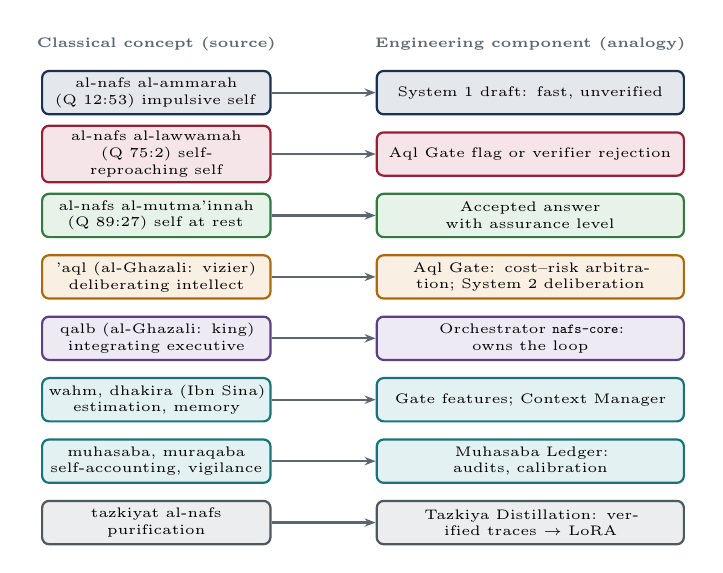
\begin{tikzpicture}[x=1cm,y=1cm]
\foreach \i/\txt/\col/\eng in {
 0/{al-nafs al-ammarah\\(Q 12:53) impulsive self}/navy/{\Sone\ draft: fast, unverified},
 1/{al-nafs al-lawwamah\\(Q 75:2) self-reproaching self}/crimson/{\Gate\ flag or verifier rejection},
 2/{al-nafs al-mutma'innah\\(Q 89:27) self at rest}/leaf/{Accepted answer with assurance level},
 3/{'aql (al-Ghazali: vizier)\\deliberating intellect}/amber/{\Gate: cost--risk arbitration; \Stwo\ deliberation},
 4/{qalb (al-Ghazali: king)\\integrating executive}/violet/{Orchestrator \texttt{nafs-core}: owns the loop},
 5/{wahm, dhakira (Ibn Sina)\\estimation, memory}/teal/{Gate features; \Mem},
 6/{muhasaba, muraqaba\\self-accounting, vigilance}/teal/{\Ledger: audits, calibration},
 7/{tazkiyat al-nafs\\purification}/slate/{\Distil: verified traces $\to$ LoRA}}
{ \node[sblk=\col,minimum width=2.9cm,text width=2.75cm] (c\i) at (0,-0.78*\i) {\txt};
  \node[sblk=\col,minimum width=3.9cm,text width=3.75cm] (e\i) at (4.75,-0.78*\i) {\eng};
  \draw[arr] (c\i)--(e\i); }
\node[font=\tiny\bfseries,text=slate] at (0,0.62) {Classical concept (source)};
\node[font=\tiny\bfseries,text=slate] at (4.75,0.62) {Engineering component (analogy)};
\end{tikzpicture}

\caption{Concept-to-component mapping. Every arrow is an analogy; component
names in code are the engineering names on the right.}
\label{fig:mapping}
\end{figure}

\subsection{Request Lifecycle}
Fig.~\ref{fig:flow} shows one request and Fig.~\ref{fig:nafs-automaton} its
state automaton. The \Mem\ assembles the prompt from the conversation and any
retrieved memory with provenance. \Sone\ produces a draft in non-thinking mode
together with $k$ cheap samples in one request (the \texttt{n} parameter of
the OpenAI-compatible API, so the prompt is prefilled once). The \Gate\
computes features: mean and minimum token log-probability of the draft,
agreement among the $k$ samples, the domain class, and, for verifiable tasks,
the verifier outcome on the draft. A calibrated model maps the features to
$\hat e_1$; the gate escalates if $L(\hat e_1-\hat e_2)>\lambda\Delta c$. A
verifiable task whose draft fails verification is never eligible for the
keep branch (this closes the draft's defect~10, where the router pseudo-code
disagreed with its prose). On escalation, \Stwo\ runs draft-blind in thinking
mode with budget $b$ and sequential sampling: each candidate is verified and
the first accepted one is returned; a rejected candidate's evidence (failing
test, counterexample, schema error) is fed into the next round, up to $R$
rounds. If the budget is exhausted the reply is an explicit abstention with
the best candidate and an uncertainty notice. Every reply carries an
\emph{assurance level}: \texttt{verified} (exact verifier passed),
\texttt{consensus} (soft agreement only), \texttt{unverified} (kept fast
draft on a non-verifiable task) or \texttt{abstained}. The decision record of
the gate and the trace of the loop are written for the \Ledger.

\begin{figure}[t]
\centering
% Request lifecycle: fast path, gate, deliberation, verification; width ~8.6cm
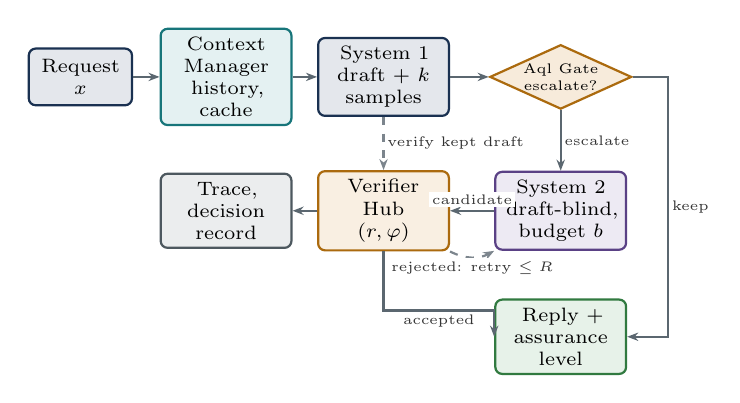
\begin{tikzpicture}[x=1cm,y=1cm]
\node[blk=navy,text width=1.1cm]   (in)  at (0.1,0)    {Request $x$};
\node[blk=teal,text width=1.45cm]   (ctx) at (1.95,0)  {\Mem\\history, cache};
\node[blk=navy,text width=1.45cm]   (s1)  at (3.95,0)  {\Sone\\draft $+$ $k$ samples};
\node[dm,minimum width=1.6cm]      (g)   at (6.2,0)  {\Gate\\escalate?};
\node[blk=violet,text width=1.45cm] (s2)  at (6.2,-1.7) {\Stwo\\draft-blind, budget $b$};
\node[blk=amber,text width=1.45cm]  (v)   at (3.95,-1.7) {\Hub\\$(r,\varphi)$};
\node[blk=slate,text width=1.45cm]  (tr)  at (1.95,-1.7) {Trace, decision record};
\node[blk=leaf,text width=1.45cm]   (out) at (6.2,-3.3) {Reply $+$ assurance level};
\draw[arr] (in)--(ctx); \draw[arr] (ctx)--(s1); \draw[arr] (s1)--(g);
\draw[arr] (g.south)--node[lab,right]{escalate}(s2.north);
\draw[arr] (g.east)--++(0.45,0)|-node[lab,pos=.25,right]{keep}(out.east);
\draw[arr] (s2)--node[lab,above=1pt]{candidate}(v);
\draw[dsh] (v.south east) to[bend right=28] node[lab,below]{rejected: retry $\le R$} (s2.south west);
\draw[arr] (v.south)--++(0,-0.75)-|node[lab,pos=.25,below]{accepted}(out.west);
\draw[dsh] (s1.south)--node[lab,right]{verify kept draft}(v.north);
\draw[arr] (v)--(tr);
\end{tikzpicture}

\caption{Request lifecycle. Solid arrows are the main path; dashed arrows are
the verification and retry edges.}
\label{fig:flow}
\end{figure}

\begin{figure}[t]
\centering
% Trace-state automaton of one request (A/L/M/T/X); width ~8.4cm
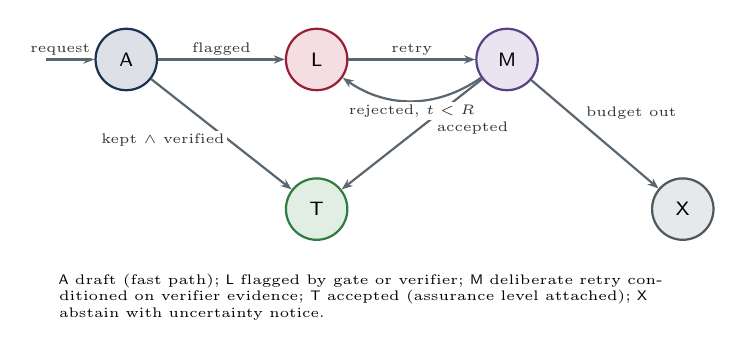
\begin{tikzpicture}[x=0.93cm,y=1cm,>=Stealth]
\node[st=navy]    (A) at (0,0)   {$\mathsf A$};
\node[st=crimson] (L) at (2.6,0) {$\mathsf L$};
\node[st=violet]  (M) at (5.2,0) {$\mathsf M$};
\node[st=leaf]    (T) at (2.6,-1.9) {$\mathsf T$};
\node[st=slate]   (X) at (7.6,-1.9) {$\mathsf X$};
\draw[arr] (-1.1,0) -- (A) node[lab,pos=0.3,above]{request};
\draw[arr] (A) -- node[lab,above]{flagged} (L);
\draw[arr] (L) -- node[lab,above]{retry} (M);
\draw[arr] (A) -- node[lab,left,pos=.55]{kept $\wedge$ verified} (T);
\draw[arr] (M) -- node[lab,below right,pos=.35]{accepted} (T);
\draw[arr] (M) to[bend left=35] node[lab,below]{rejected, $t<R$} (L);
\draw[arr] (M) -- node[lab,above right,pos=.4]{budget out} (X);
\node[font=\tiny,align=left,anchor=north west,text width=7.9cm] at (-1.05,-2.6)
 {$\mathsf A$ draft (fast path); $\mathsf L$ flagged by gate or verifier; $\mathsf M$ deliberate retry conditioned on verifier evidence;
  $\mathsf T$ accepted (assurance level attached); $\mathsf X$ abstain with uncertainty notice.};
\end{tikzpicture}

\caption{Trace-state automaton of one request. The three Qur'anic stage names
are used as mnemonics for $\mathsf A$, $\mathsf L$ and $\mathsf T$; the
automaton is a bounded retry loop (Lemma~\ref{lem:termination}).}
\label{fig:nafs-automaton}
\end{figure}

\subsection{Components}
\label{sec:components}
\begin{itemize}
\item \textbf{\Gw\ (\texttt{nafs-gateway}).} HTTP API (OpenAPI 3.1), SSE
streaming of tokens and of controller events, WebSocket chat rooms,
authentication, rate limits, Prometheus metrics.
\item \textbf{Orchestrator and \Gate\ (\texttt{nafs-core}).} Implements the
automaton, the gate, sequential verified sampling, budget forcing, timeouts
and fallbacks; emits the decision record.
\item \textbf{\Sone\ and \Stwo\ backends.} Two OpenAI-compatible model
servers (or one server with two modes in the single-model profile), reached
over HTTP with retry and backpressure.
\item \textbf{\Hub\ (\texttt{nafs-verify}).} Exact verifiers: code sandbox
(subprocess with CPU, memory, wall-clock and network limits), numeric and
symbolic mathematics (reference-answer equality, SymPy via a sidecar), JSON
Schema validation, format checks. Soft verifiers: rubric judge (the \Stwo\
model in non-thinking mode at temperature~0) and sample consensus. Each
verifier publishes $(r,\varphi)$ from mutation tests.
\item \textbf{\Mem\ (\texttt{nafs-memory}).} Conversation store (SQLite),
prompt assembly within a context cap, prompt-cache affinity hints for the
model server, episodic trace store (JSONL), and a retrieval index built with
Qwen3-Embedding-0.6B when retrieval is enabled.
\item \textbf{\Ledger.} Offline job that aggregates traces and the $5\%$ audit
stream into per-domain calibration tables (escalation rate, $\hat e_1$
calibration error, verifier acceptance rates, latency quantiles), keyed by
model and adapter hash; feeds the dashboard and the gate's recalibration.
\item \textbf{\Harness\ (\texttt{nafs-eval}) and performance console
(\texttt{nafs-bench}).} Dataset loaders, metric definitions, paired
statistical tests, load generation, and report export.
\item \textbf{Web UI (\texttt{nafs-web}).} Chat room with the assurance level
and the reasoning mode visible per message, a performance-test console, and an
evaluation dashboard; server-rendered HTML with htmx for streaming updates.
\item \textbf{\Distil\ (Python, GPU).} Dataset builder from verified traces,
Unsloth LoRA training, promotion gate, GGUF export.
\end{itemize}

\begin{figure}[t]
\centering
% System architecture (single-node CPU baseline); width ~8.6cm
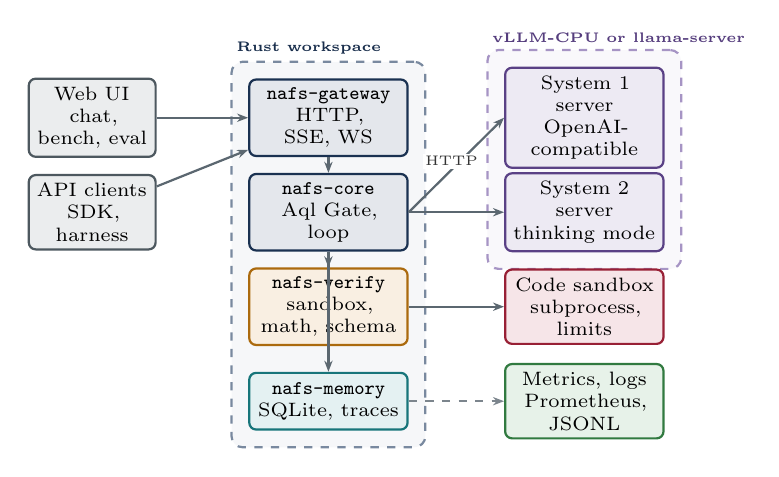
\begin{tikzpicture}[x=1cm,y=1cm]
\node[blk=slate,text width=1.4cm] (ui) at (0.1,0) {Web UI\\chat, bench, eval};
\node[blk=slate,text width=1.4cm] (cli) at (0.1,-1.2) {API clients\\SDK, harness};
\node[blk=navy,text width=1.8cm] (api) at (3.1,0) {\texttt{nafs-gateway}\\HTTP, SSE, WS};
\node[blk=navy,text width=1.8cm] (core) at (3.1,-1.2) {\texttt{nafs-core}\\\Gate, loop};
\node[blk=amber,text width=1.8cm] (hub) at (3.1,-2.4) {\texttt{nafs-verify}\\sandbox, math, schema};
\node[blk=teal,text width=1.8cm] (mem) at (3.1,-3.6) {\texttt{nafs-memory}\\SQLite, traces};
\node[blk=violet,text width=1.8cm] (b1) at (6.35,0) {\Sone\ server\\OpenAI-compatible};
\node[blk=violet,text width=1.8cm] (b2) at (6.35,-1.2) {\Stwo\ server\\thinking mode};
\node[blk=crimson,text width=1.8cm] (sb) at (6.35,-2.4) {Code sandbox\\subprocess, limits};
\node[blk=leaf,text width=1.8cm] (obs) at (6.35,-3.6) {Metrics, logs\\Prometheus, JSONL};
\begin{scope}[on background layer]
\node[grp=navy,fit=(api)(core)(hub)(mem),inner sep=6pt] (gw) {};
\node[grp=violet,fit=(b1)(b2),inner sep=6pt] (srv) {};
\end{scope}
\node[grplab=navy,anchor=south west] at (gw.north west) {Rust workspace};
\node[grplab=violet,anchor=south west] at (srv.north west) {vLLM-CPU or llama-server};
\draw[arr] (ui)--(api); \draw[arr] (cli)--(api);
\draw[arr] (api)--(core); \draw[arr] (core)--(hub); \draw[arr] (core)--(mem);
\draw[arr] (core.east)--node[lab,above,pos=.45]{HTTP}(b1.west);
\draw[arr] (core.east)--(b2.west);
\draw[arr] (hub)--(sb);
\draw[dsh] (mem)--(obs);
\end{tikzpicture}

\caption{System architecture, single-node CPU baseline. The GPU scale-out
variant replaces the model servers with vLLM on CUDA and keeps every other
component unchanged.}
\label{fig:arch}
\end{figure}

\subsection{Model Profiles}
\label{sec:models}
Table~\ref{tab:profiles} defines three profiles. Profile~A is the reference:
two dense Qwen3 checkpoints, one per role, chosen because dense
grouped-query attention has the most mature CPU kernels, official GGUF files
exist, and both are on vLLM's validated CPU list. Profile~B serves one
switchable Qwen3-4B for both roles, halving resident memory at the price of a
slower fast path; the gate then decides \emph{whether to think}, exactly the
decision studied by the adaptive-thinking literature. Profile~C is the
upgrade path to Qwen3.5, which is stronger and multimodal but uses hybrid
linear attention whose CPU kernels are newer and, on AVX2 without
AVX-512-BF16 or AMX, unaccelerated in vLLM; Phase~0 of the roadmap benchmarks
it against Profile~A on the target machine before any commitment. The
upgrade decision is a go/no-go gate with a measurable criterion.

\begin{table}[t]
\caption{Model profiles (Hugging Face IDs verified 2026-10-18; sizes are GGUF file sizes)}
\label{tab:profiles}
\centering\scriptsize
\begin{tabular}{@{}p{0.7cm}>{\raggedright\arraybackslash}p{3.6cm}>{\raggedright\arraybackslash}p{3.6cm}@{}}
\toprule
Profile & \Sone & \Stwo \\
\midrule
A (ref.) & \texttt{Qwen/\allowbreak Qwen3-1.7B}, GGUF Q4\_K\_M 1.3\,GB (\texttt{unsloth/\allowbreak Qwen3-1.7B-GGUF}) or Q8\_0 1.8\,GB (\texttt{Qwen/\allowbreak Qwen3-1.7B-GGUF}); thinking off & \texttt{Qwen/\allowbreak Qwen3-4B-\allowbreak Thinking-2507}, GGUF Q4\_K\_M 2.5\,GB (\texttt{unsloth/\allowbreak Qwen3-4B-\allowbreak Thinking-2507-\allowbreak GGUF}); 262K context \\
B (min.) & \texttt{Qwen/\allowbreak Qwen3-4B} Q4\_K\_M 2.5\,GB (\texttt{Qwen/\allowbreak Qwen3-4B-GGUF}), \texttt{enable\_thinking=false} & same weights, \texttt{enable\_thinking=true} \\
C (upgr.) & \texttt{Qwen/\allowbreak Qwen3.5-2B} Q4\_K\_M 1.3\,GB (\texttt{unsloth/\allowbreak Qwen3.5-2B-GGUF}) & \texttt{Qwen/\allowbreak Qwen3.5-4B} Q4\_K\_M 2.7\,GB (\texttt{unsloth/\allowbreak Qwen3.5-4B-GGUF}) \\
\midrule
\multicolumn{3}{@{}p{8.2cm}@{}}{Judge: the \Stwo\ model in non-thinking mode. Embeddings: \texttt{Qwen/\allowbreak Qwen3-Embedding-0.6B-GGUF} Q8\_0. All Apache-2.0. GPU scale-out: the same IDs in BF16 or AWQ under vLLM CUDA, with \texttt{Qwen/Qwen3-8B} as the \Stwo\ option.} \\
\bottomrule
\end{tabular}
\end{table}

\subsection{Deployment Topology}
The CPU baseline is a single node: one gateway process, one or two model
servers pinned to the physical cores (the gateway reserves none, since the
gateway's own CPU use is small and bursty), a sandbox runner, SQLite and
JSONL on local disk. The model servers are either \texttt{llama-server}
(macOS or any x86) or vLLM-CPU (Linux, AVX-512 recommended), both behind the
same OpenAI-compatible API, so the Rust code has one backend trait and two
thin implementations. The optional GPU scale-out variant moves the model
servers to vLLM on CUDA with both models resident, raises $N$ and the
thinking budget, and enables EAGLE or multi-token-prediction speculative
decoding; the gateway, verifiers, memory and UI are unchanged.

\subsection{What Changed from the Draft}
The draft's twelve validation results are retained where exact (precision,
coverage, cascade cost, router threshold, consensus, value-score algebra,
coupling, audit, measurement floors, distillation noise, capacity, cascade
identity) and are restated here with explicit assumptions. We added the
miscalibration bound, the frontier proposition, the optimal-stopping cap, the
two refinement-loop theorems, the plurality limit, the roofline and the
thinking-budget condition. We removed the mapping of the Active Intellect to
``external verifiers'' and of \emph{ilham} to any component, following the
guidance in Section~\ref{sec:islamic}; we replaced the GPU roster with CPU
profiles; and we turned the draft's ten defects into requirements with tests
in the specification.

\section{Implementation Stack}
\label{sec:stack}

\subsection{Model Serving}
\textbf{vLLM.} vLLM \cite{kwon2023pagedattention} is the specified serving
layer for the Linux deployment profile. Its x86 CPU backend requires Linux,
supports FP32, FP16 and BF16 with AWQ, GPTQ and INT8 W8A8 quantisation,
recommends AVX-512 and offers ``limited features'' on AVX2; pre-built CPU
wheels and the \texttt{vllm/vllm-openai-cpu} image exist. Qwen3-1.7B, 4B and
8B are on its validated CPU model list. The CPU backend implements hybrid
Gated-DeltaNet models, but the accelerated path needs AMX or AVX-512-BF16;
elsewhere it falls back to a generic path. At the time of writing the latest
published release is v0.31.0 (v0.32.0 is a tag, not a release); the
specification pins 0.31.0. vLLM exposes OpenAI-compatible chat completions
with \texttt{logprobs} and \texttt{top\_logprobs}, the \texttt{n} parameter,
a \texttt{qwen3} reasoning parser that separates \texttt{reasoning\_content},
and \texttt{chat\_template\_kwargs} for \texttt{enable\_thinking}; these are
exactly the hooks the gate needs. On the macOS Intel reference machine vLLM
runs only inside a Linux container.

\textbf{llama.cpp.} \texttt{llama-server} (release v0.7.0, October 2026) is
the mandated fallback and the primary engine on the reference machine: GGUF
weights, a mature AVX2 path, OpenAI-compatible chat completions with SSE
streaming and \texttt{logprobs}, \texttt{--reasoning-format} to separate
reasoning, \texttt{--reasoning-budget} for budget forcing, n-gram speculative
decoding without a draft model (\texttt{--spec-type ngram-simple}), and
explicit thread pinning. Both engines present the same HTTP contract, so the
Rust gateway has a single backend trait.

\textbf{Ollama} is convenient for demonstrations but its OpenAI endpoint does
not return log-probabilities, which the gate requires; it is therefore not a
supported backend.

\subsection{Fine-Tuning}
Unsloth (2026.10.6) trains with LoRA and QLoRA two to five times faster than
baseline PEFT and exports merged weights to GGUF directly. Its core trainer
requires a torch accelerator: the device-selection code raises ``You need a
GPU'' on CPU-only hosts, and the documented CPU support covers inference and
data preparation, not training. The feasible path is therefore: collect and
filter traces on the CPU machine, train on a rented GPU (a 16\,GB T4 covers
QLoRA on Qwen3-1.7B and 4B \cite{dettmers2023qlora,hu2022lora}, and BF16
LoRA on Qwen3.5 up to 4B; Unsloth advises against 4-bit training for
Qwen3.5), export GGUF, and run the promotion gate and all evaluation on CPU.
Unsloth's default hyperparameters (rank 16--32, $\alpha=r$, learning rate
$2\times10^{-4}$, one to three epochs, effective batch 16, dropout 0, all
attention and MLP projections) are the starting point of the training
specification.

\subsection{Rust Web Application}
Table~\ref{tab:crates} lists the crates and the versions verified on
crates.io on 2026-10-18. \textbf{axum} on \textbf{tokio} and \textbf{tower}
is the mainstream, well-maintained choice for an async HTTP service with
SSE (\texttt{axum::response::Sse}) and WebSockets built in;
\textbf{reqwest} with \texttt{eventsource-stream} consumes the model
servers' SSE; \textbf{serde} and \textbf{schemars} give JSON (de)serialisation
and JSON-Schema generation from the same Rust types that the OpenAPI document
is generated from with \textbf{utoipa}; \textbf{sqlx} with SQLite gives
compile-time-checked queries without a database server; \textbf{tracing}
with OpenTelemetry export and \textbf{metrics-exporter-prometheus} provide
observability; \textbf{askama} templates with \textbf{htmx} keep the
front end server-rendered and dependency-light (a single-page framework such
as Leptos is an option for a later phase, not a requirement); \textbf{goose}
provides load generation for the performance console and \textbf{criterion}
micro-benchmarks. The toolchain is pinned to the stable release current at
project start (1.96 on the reference machine; 1.99 is current upstream).

\begin{table}[t]
\caption{Rust crates (versions on crates.io, 2026-10-18)}
\label{tab:crates}
\centering\scriptsize
\begin{tabular}{@{}p{2.6cm}p{1.6cm}p{3.6cm}@{}}
\toprule
Crate & Version & Role \\
\midrule
tokio & 1.53.3 & async runtime \\
axum & 0.8.9 & HTTP routing, SSE, WebSocket \\
tower, tower-http & 0.5.3, 0.7.1 & middleware: timeouts, limits, CORS, compression \\
hyper & 1.12.0 & HTTP/1.1 and HTTP/2 \\
reqwest & 0.13.5 & client to model servers (streaming) \\
eventsource-stream & 0.2.3 & SSE parsing of upstream streams \\
serde, serde\_json & 1.0.229, 1.0.154 & (de)serialisation \\
schemars & 1.2.3 & JSON Schema from types \\
jsonschema & 0.59.0 & schema verifier \\
utoipa, utoipa-\allowbreak swagger-ui & 6.0.0, 10.0.1 & OpenAPI 3.1 generation and docs UI \\
sqlx & 0.9.0 & SQLite access, migrations \\
tracing, tracing-subscriber & 0.1.44, 0.3.23 & structured logs and spans \\
opentelemetry, tracing-\allowbreak opentelemetry & 0.33.1, 0.34.0 & trace export \\
metrics, metrics-\allowbreak exporter-\allowbreak prometheus & 0.24.6, 0.18.3 & metrics \\
askama & 0.16.1 & HTML templates \\
clap, figment & 4.6.7, 0.10.19 & CLI and layered configuration \\
thiserror, anyhow & 2.0.21, 1.0.104 & error taxonomy \\
uuid, chrono & 1.28.0, 0.4.45 & identifiers, time \\
governor & 0.10.4 & rate limiting \\
criterion, goose & 0.8.2, 0.18.1 & micro-benchmarks, load tests \\
\bottomrule
\end{tabular}
\end{table}

\subsection{Reference Machine and Measured Feasibility}
\label{sec:feasibility}
The reference machine is an Intel Core i3-8100 (four cores, no simultaneous
multithreading, AVX2 and FMA, no AVX-512), 32\,GB of DDR4, macOS~15.4.1. We
built llama.cpp from source (commit \texttt{797de63}, 2026-10-17) and ran
\texttt{llama-bench} with four threads, 512-token prefill and 128-token
decode, three repetitions. Table~\ref{tab:measured} reports the results. The
Qwen3-1.7B decode rate of $15.5$ tokens/s against a 1.26\,GiB weight file
implies an effective bandwidth of about $20$\,GB/s, roughly half the
theoretical $38.4$\,GB/s of dual-channel DDR4-2400, which is in line with the
roofline of Proposition~\ref{prop:roofline} and with published AVX2 data
points. We also confirmed, through Ollama, that Qwen3-1.7B generates in both
thinking and non-thinking modes on this machine; a 512-token thinking cap was
exhausted on a simple arithmetic question before the answer was produced,
which is the empirical reason the controller forces the answer when the
budget is reached (Proposition~\ref{prop:budget}). We also exercised \texttt{llama-server} through its OpenAI-compatible API with
Qwen3-1.7B: per-token log-probabilities are returned with \texttt{logprobs};
the \texttt{n} parameter is capped by the number of server slots, so the
gate's $k$ cheap samples are issued as $k$ parallel requests against
$k$ slots (four 12-token samples completed in 3.0\,s with 47 of 48 prompt
tokens served from the prompt cache); \texttt{enable\_thinking} toggles the
mode per request; \texttt{--reasoning-budget 256} closed the reasoning span
after 256 tokens and the model then produced an answer; and SSE streaming
delivered chunked deltas. These are the exact hooks the specification relies
on. We did not run vLLM on the
reference machine because the Docker daemon was not running; the
specification's vLLM configuration is taken from its documentation and is
marked as untested on this machine.

\begin{table}[t]
\caption{Measured throughput on the reference machine (llama.cpp, 4 threads; mean $\pm$ s.d. over 3 runs)}
\label{tab:measured}
\centering\scriptsize
\begin{tabular}{@{}llrr@{}}
\toprule
Model (GGUF) & Size & Prefill tok/s & Decode tok/s \\
\midrule
Qwen3-0.6B Q8\_0 & 604\,MiB & $180.6\pm2.4$ & $32.6\pm1.8$ \\
Qwen3-1.7B Q4\_K\_M & 1.26\,GiB & $94.1\pm9.5$ & $15.5\pm3.4$ \\
\MEASUREDROWS
\bottomrule
\end{tabular}
\end{table}

From these measurements and the roofline we derive the CPU-baseline
targets of the specification: a fast-path first token under two seconds for
prompts up to 1\,000 tokens with prompt caching, a fast-path reply of 150
tokens in about ten seconds, and a slow-path reply with a 1\,024-token
thinking budget on the 4B model in about two to three minutes; the latter
is acceptable for a demonstration and for batch evaluation, and is the
reason the roadmap keeps interactive use of \Stwo\ optional until the GPU
variant exists.

\section{Features and Capabilities}
\label{sec:features}
\begin{itemize}
\item \textbf{Dual-process chat.} Every reply shows which path produced it,
the assurance level, the thinking budget used and the cost; the user can move
a single ``speed--care'' control, which sets $\lambda$
(Proposition~\ref{prop:frontier}).
\item \textbf{Verified answers on code, mathematics and structured output},
with precision bounded by the verifier (Theorem~\ref{thm:precision}), and
evidence-fed retries (Theorem~\ref{thm:gatedloop}).
\item \textbf{Calibrated abstention.} When the budget is exhausted the system
says so, returns the best candidate with an uncertainty notice, and never
upgrades consensus to verification (Theorem~\ref{thm:plurality}).
\item \textbf{Honest self-description.} A per-domain capability table from
audited traces, with unmeasured domains marked as such
(Proposition~\ref{prop:audit}).
\item \textbf{Performance console.} Load tests against the gateway with
latency quantiles, throughput, escalation rate and cost per request, run from
the browser.
\item \textbf{Evaluation dashboard.} Benchmark runs with paired comparisons
against the fast-only and slow-only baselines, confidence intervals, routing
accuracy and calibration plots, and the go/no-go status of each roadmap gate.
\item \textbf{Gradual distillation.} Verified slow-path traces become
training data for the fast path under a statistically sized promotion gate
with human sign-off (Proposition~\ref{prop:distill}).
\item \textbf{Backend portability.} The same gateway runs against
llama-server on a laptop and vLLM on a server, CPU or GPU.
\end{itemize}
Honest limits: non-verifiable domains never exceed the \texttt{consensus}
assurance level; the fast and slow paths share a model family, so their errors
are correlated and the collision term of Proposition~\ref{prop:collision} is
measured, not assumed small; on the reference machine the slow path is not
interactive.

\section{Specification and Roadmap Summary}
\label{sec:spec}
The companion \emph{Technical Specification} and \emph{Development Roadmap}
are standalone documents built from the same sources as this report; this
section summarises them so that the report is self-contained.

\subsection{Specification}
The specification uses RFC~2119 keywords and gives every requirement an
identifier: functional (FR), non-functional (NFR), interface (IF), model
(MR), training (TR), security (SR), operations (OR) and evaluation (ER). The
requirement catalogue has \NREQ\ entries; each is traced to the result or
design decision that motivates it, to the component that implements it and
to the test that verifies it. Key normative content:
\begin{itemize}
\item \textbf{Gate (FR-010--FR-014).} The controller MUST compute the
decision of Theorem~\ref{thm:gate} from a calibrated estimator and a
configured cost ratio, MUST never keep a verifiable draft that failed
verification, and MUST write a decision record with the features, estimates
and thresholds used.
\item \textbf{Deliberation (FR-020--FR-024).} Sequential verified sampling
with configured caps $N$, $R$ and budget $b$ per domain derived from the
Phase-0 fit; draft-blind by default; budget forcing on exhaustion; abstention
with notice.
\item \textbf{Verification (FR-030--FR-033).} Exact verifiers accept at
threshold $1.0$; every verifier publishes $(r,\varphi)$; assurance levels are
attached to every reply; consensus never writes training data.
\item \textbf{Self-model (FR-040--FR-042).} A $5\%$ audit stream; unmeasured
capabilities reported as unmeasured; statistics keyed by model and adapter
hash.
\item \textbf{Distillation (TR-001--TR-008).} Data schema, filtering, Unsloth
LoRA configuration, GPU path, promotion gate with confidence bounds and
held-out verifier, human sign-off, GGUF export.
\item \textbf{Targets (NFR-001--NFR-012).} Hard latency bound from
Lemma~\ref{lem:termination}; fast-path first token under two seconds and
150-token reply within twelve seconds at p95 on the reference machine;
resident memory under 8\,GB for Profile~A; reproducible builds; structured
telemetry. All targets are labelled as targets.
\item \textbf{Interfaces (IF-001--IF-010).} OpenAPI 3.1 for the gateway
with SSE streaming and a \texttt{reasoning\_mode} field on every reply; JSON
Schemas for the request, reply, decision record and trace; the backend
contract to vLLM and llama-server with retry, timeout and backpressure
policy.
\end{itemize}
Machine-readable artefacts accompany the document: \texttt{openapi.yaml},
JSON Schemas, a sample vLLM launch configuration and llama-server command,
a Cargo workspace skeleton and a sample configuration file, all validated
with standard tools.

\subsection{Roadmap}
Fig.~\ref{fig:gantt} shows the seven phases and their gates; effort and dates
are estimates. Phase~0 (foundations, weeks 0--3) delivers the serving
baseline on the reference machine and the $4\,600$-task measurement run.
Phase~1 (CPU MVP, weeks 3--8) delivers the gateway, both paths behind a
fixed-rule gate, the chat UI and the minimal verifier hub, which is the
smallest build that demonstrates the idea end to end. Phase~2 (gate and
loop, weeks 8--13) replaces the fixed rule with the calibrated gate and adds
the verified retry loop and the audit stream; its exit gate is the
non-inferiority test at three points. Phase~3 (fine-tuning, weeks 12--18)
runs the first distillation cycle on a rented GPU under the promotion gate.
Phase~4 (evaluation suite and performance console, weeks 15--21) completes
the dashboard and the load tests. Phase~5 (hardening and optional GPU
scale-out, weeks 20--25) adds security hardening, the vLLM CUDA profile and
the Qwen3.5 upgrade decision. Phase~6 (release and publication, weeks
25--28) delivers the one-point non-inferiority gate, documentation and the
research write-up. Phase~7 (CPU inference performance, added after the
first six phases were implemented) attributes latency to stages, tunes the
engine under interleaved A/B tests, adds early escalation, and prepares
EAGLE-3 speculative heads and repacked weight formats. The MVP is specified with acceptance tests; every phase
has measurable entry and exit criteria, a risk register with early-warning
signals, and a research-to-engineering table that schedules hypotheses
H1--H7.

\begin{figure}[t]
\centering
% Roadmap timeline (weeks); width ~8.6cm; estimates. Phase 7 was added after Phases 0-6 were implemented.
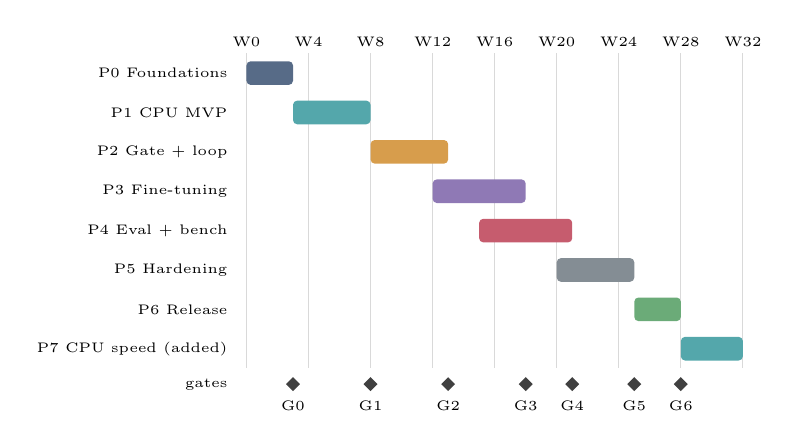
\begin{tikzpicture}[x=0.197cm,y=0.5cm]
\foreach \w in {0,4,...,32}{\draw[black!15] (\w,0.3)--(\w,-7.7);\node[font=\tiny] at (\w,0.6){W\w};}
\foreach \ii/\lbl/\st/\en/\col in {
 0/{P0 Foundations}/0/3/navy,
 1/{P1 CPU MVP}/3/8/teal,
 2/{P2 Gate + loop}/8/13/amber,
 3/{P3 Fine-tuning}/12/18/violet,
 4/{P4 Eval + bench}/15/21/crimson,
 5/{P5 Hardening}/20/25/slate,
 6/{P6 Release}/25/28/leaf,
 7/{P7 CPU speed (added)}/28/32/teal}
 {\node[anchor=east,font=\tiny] at (-0.6,-\ii-0.2){\lbl};
  \fill[\col!75,rounded corners=1.5pt](\st,-\ii-0.5) rectangle (\en,-\ii+0.1);}
\foreach \x/\n in {3/G0,8/G1,13/G2,18/G3,21/G4,25/G5,28/G6}{\node[diamond,fill=black!75,inner sep=1.3pt] (g\n) at (\x,-8.1){};\node[font=\tiny,below=1pt] at (\x,-8.2){\n};}
\node[anchor=east,font=\tiny] at (-0.6,-8.1){gates};
\end{tikzpicture}

\caption{Roadmap timeline (weeks; estimates). Diamonds are decision gates
G0--G6 with go/no-go criteria defined in the roadmap document.}
\label{fig:gantt}
\end{figure}

\begin{figure}[t]
\centering
% Training (GPU) and serving (CPU) pipeline; width ~8.6cm
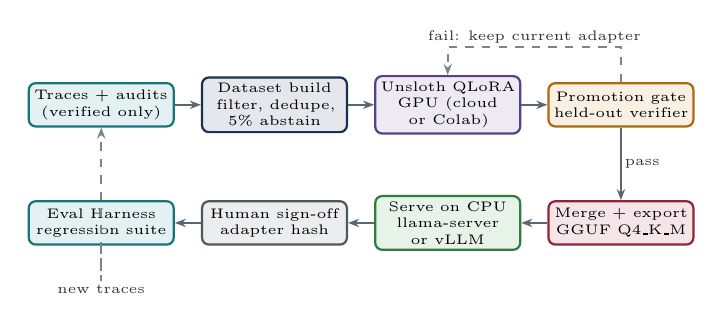
\begin{tikzpicture}[x=1cm,y=1cm]
\node[sblk=teal,text width=1.7cm]   (tr) at (0,0)   {Traces $+$ audits\\(verified only)};
\node[sblk=navy,text width=1.7cm]   (ds) at (2.2,0) {Dataset build\\filter, dedupe, 5\% abstain};
\node[sblk=violet,text width=1.7cm] (ft) at (4.4,0) {Unsloth QLoRA\\GPU (cloud or Colab)};
\node[sblk=amber,text width=1.7cm]  (gate) at (6.6,0) {Promotion gate\\held-out verifier};
\node[sblk=crimson,text width=1.7cm](exp) at (6.6,-1.5) {Merge $+$ export\\GGUF Q4\_K\_M};
\node[sblk=leaf,text width=1.7cm]   (srv) at (4.4,-1.5) {Serve on CPU\\llama-server or vLLM};
\node[sblk=slate,text width=1.7cm]  (hum) at (2.2,-1.5) {Human sign-off\\adapter hash};
\node[sblk=teal,text width=1.7cm]   (ev) at (0,-1.5) {\Harness\\regression suite};
\draw[arr] (tr)--(ds); \draw[arr] (ds)--(ft); \draw[arr] (ft)--(gate);
\draw[arr] (gate)--node[lab,right]{pass}(exp); \draw[arr] (exp)--(srv); \draw[arr] (srv)--(hum);
\draw[arr] (hum)--(ev);
\draw[dsh] (ev.south)--++(0,-0.45)-|node[lab,pos=.25,below]{new traces}(tr.south);
\draw[dsh] (gate.north)--++(0,0.45)-|node[lab,pos=.25,above]{fail: keep current adapter}(ft.north);
\end{tikzpicture}

\caption{Training and serving pipeline. Training runs on a rented GPU;
everything else runs on CPU.}
\label{fig:pipeline}
\end{figure}

\section{Evaluation Plan and Metrics}
\label{sec:eval}
No result in this section has been measured; the section defines what will be
measured, how, and what counts as success. The full definitions, formulas and
test plans are in the specification (Section~10 there).

\subsection{Metrics}
\begin{itemize}
\item \textbf{Quality.} Exact-match or test-pass accuracy on verifiable
benchmarks; pairwise win rate against the slow-only baseline by a held-out
judge on non-verifiable prompts; abstention rate and accuracy among
non-abstained answers (selective accuracy at coverage).
\item \textbf{Routing.} Escalation rate $g$; routing accuracy, defined as the
fraction of requests on which the gate's decision agrees with the oracle
decision of Theorem~\ref{thm:gate} computed from labelled outcomes; the
area under the cost--accuracy curve as $\lambda$ varies
(Proposition~\ref{prop:frontier}).
\item \textbf{Cost and latency.} Tokens and CPU-seconds per request by path;
time to first token and total latency at p50, p95 and p99; throughput under
load.
\item \textbf{Calibration.} Expected calibration error of $\hat e_1$ with
five bins and $n\ge2\,900$ (the noise floor of a ten-bin estimate at $n=500$
is $0.034$, above the target), and Brier score.
\item \textbf{Verifier quality.} $(r,\varphi)$ per verifier from mutation
tests, with Clopper--Pearson intervals \cite{clopper1934}.
\item \textbf{Faithfulness.} Agreement between the reasoning trace and the
answer on perturbation tests \cite{turpin2023unfaithful,lanham2023faithfulness},
and adoption rate of a wrong fast draft by the slow path
(Proposition~\ref{prop:collision}).
\item \textbf{Robustness.} Accuracy under paraphrase and under prompt
injection probes \cite{greshake2023injection,zou2023universal,wei2023jailbroken}.
\end{itemize}

\subsection{Benchmarks}
GSM8K \cite{cobbe2021gsm8k} and MATH \cite{hendrycks2021math} (mathematics,
exact verifiers), HumanEval \cite{chen2021humaneval} and MBPP
\cite{austin2021mbpp} (code, test verifiers), a JSON-Schema task set generated
from public schemas (format verifier), MMLU and GPQA
\cite{hendrycks2021mmlu,rein2024gpqa} (knowledge, label verifier),
TruthfulQA and SimpleQA \cite{lin2022truthfulqa,wei2024simpleqa} (factuality),
BIG-Bench Hard \cite{suzgun2022bbh} and LiveCodeBench
\cite{jain2025livecodebench} as contamination-resistant checks, and MT-Bench
style judged conversations \cite{zheng2023mtbench}. Licences are MIT,
Apache-2.0 or CC-BY-4.0 (GPQA is gated). Public routing data from RouteLLM
\cite{ong2025routellm} seeds the gate's calibration set.

\subsection{Protocol}
Phase~0 runs the fast-only and slow-only baselines on at least $4\,600$ tasks
across domains (Proposition~\ref{prop:samples}) to estimate $q$, $(r,\varphi)$,
$e_1(s)$, $e_2(s)$, the cost ratio and the discordance rate. Every later
comparison is paired on the same tasks, reports the difference with a
$95\%$ confidence interval, and uses a non-inferiority margin of three points
(about $700$ pairs) during development and one point (about $6\,200$ pairs)
for release. Gates for rates that must be below a threshold use the
zero-failure binomial rule or the Clopper--Pearson upper bound. Drift in the
self-model is monitored with a CUSUM chart \cite{page1954cusum} and a negative
control. Multiple comparisons across five domains use a Bonferroni-corrected
$z=2.326$.

\begin{figure}[t]
\centering
% Evaluation workflow; width ~8.6cm
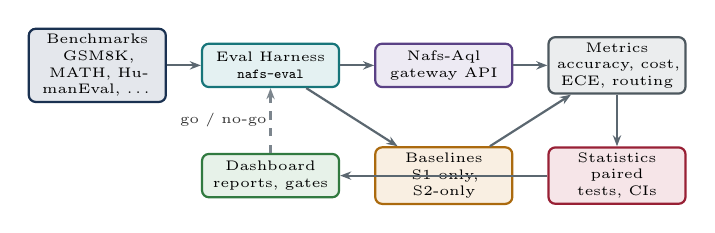
\begin{tikzpicture}[x=1cm,y=1cm]
\node[sblk=navy,text width=1.6cm]   (ds) at (0,0)    {Benchmarks\\GSM8K, MATH, HumanEval, \ldots};
\node[sblk=teal,text width=1.6cm]   (h)  at (2.2,0)  {\Harness\\\texttt{nafs-eval}};
\node[sblk=violet,text width=1.6cm] (sys) at (4.4,0) {\Sys\\gateway API};
\node[sblk=amber,text width=1.6cm]  (bl) at (4.4,-1.4) {Baselines\\S1-only, S2-only};
\node[sblk=slate,text width=1.6cm]  (m)  at (6.6,0)  {Metrics\\accuracy, cost, ECE, routing};
\node[sblk=crimson,text width=1.6cm](st) at (6.6,-1.4) {Statistics\\paired tests, CIs};
\node[sblk=leaf,text width=1.6cm]   (db) at (2.2,-1.4) {Dashboard\\reports, gates};
\draw[arr] (ds)--(h); \draw[arr] (h)--(sys); \draw[arr] (h)--(bl); \draw[arr] (sys)--(m); \draw[arr] (bl)--(m);
\draw[arr] (m)--(st); \draw[arr] (st)--(db); \draw[dsh] (db)--node[lab,left]{go / no-go}(h);
\end{tikzpicture}

\caption{Evaluation workflow. The harness drives the system and the two
baselines through the same API and the dashboard shows gate status.}
\label{fig:eval}
\end{figure}

\subsection{Hypotheses Scheduled for Validation}
H1: the calibrated gate achieves at least $70\%$ routing accuracy against the
oracle at $g\le0.3$ (Phase~2). H2: at matched accuracy the cascade costs at
most $60\%$ of the slow-only baseline on the Phase-0 suite (Phase~2). H3: per-task
acceptance rates are adequately fitted by a Beta distribution per domain,
judged by a goodness-of-fit test (Phase~2). H4: slow-path accuracy is concave
in the thinking budget on each domain (Phase~0). H5: the draft-blind slow
path adopts a wrong fast draft in fewer than $5\%$ of trials at $95\%$
confidence over at least $200$ trials (Phase~2). H6: one round of distillation
yields a lower-confidence-bound gain above zero on a held-out verifier without
a per-domain regression beyond one point (Phase~3). H7: Qwen3.5 hybrid
models decode at no less than $70\%$ of the speed of same-size dense Qwen3
models on the target CPU (Phase~0, gate for Profile~C).

\section{Implementation and Measured Results}
\label{sec:impl}
This section reports the system as built and what it measured, as of 18 October 2026. Phases~0--6 of the
roadmap are implemented on the CPU reference machine, and a Phase~7 on CPU inference performance was added
(Section~\ref{sec:impl:perf}). GPU training and GPU scale-out were deferred. Every number below is generated by
\texttt{scripts/gen\_publication.py} from stored runs and evidence files. The machine was shared with other
workloads (load average 6--18), so absolute speeds are lower bounds and small effects are within noise. Sample
sizes are far below the release gates of Section~\ref{sec:eval}, so the results are indicative.

\subsection{The system as built}
The Rust workspace has eight crates: the gateway (axum), the orchestrator (\texttt{nafs-core}), verifiers with
a sandbox, memory (SQLite, BM25 retrieval), evaluation and statistics, load testing, the shared types, and an
embedded web interface. The gateway serves 50 documented endpoints (OpenAPI~1.5) and an OpenAI-compatible chat
API. System~1 is Qwen3-1.7B and System~2 Qwen3-4B-Thinking-2507, both in Q4\_K\_M on llama-server; a vLLM-CPU
profile runs the same API in a Linux VM or container.

The web interface (Fig.~\ref{fig:ui-chat}) has seven pages:
\begin{itemize}
\item \textbf{Chat:} streaming answers with the automaton strip (A~$\to$~L~$\to$~M~$\to$~T/X), assurance badges,
a one-line reason from the gate, an inspector with the decision record and a per-stage latency waterfall, and
``Both'' trials in which a person compares the System~1 and System~2 answers;
\item \textbf{Lab:} experiment presets, paired statistics, the roadmap gates and a pooled policy map;
\item \textbf{Muhasaba:} gate mode and calibration, verifier quality, the capability ledger, drift and alerts;
\item \textbf{Tazkiya:} distillation readiness, the review queue and the model registry;
\item \textbf{Rooms}, \textbf{Performance} and \textbf{System}.
\end{itemize}

\begin{figure*}[t]
\centering
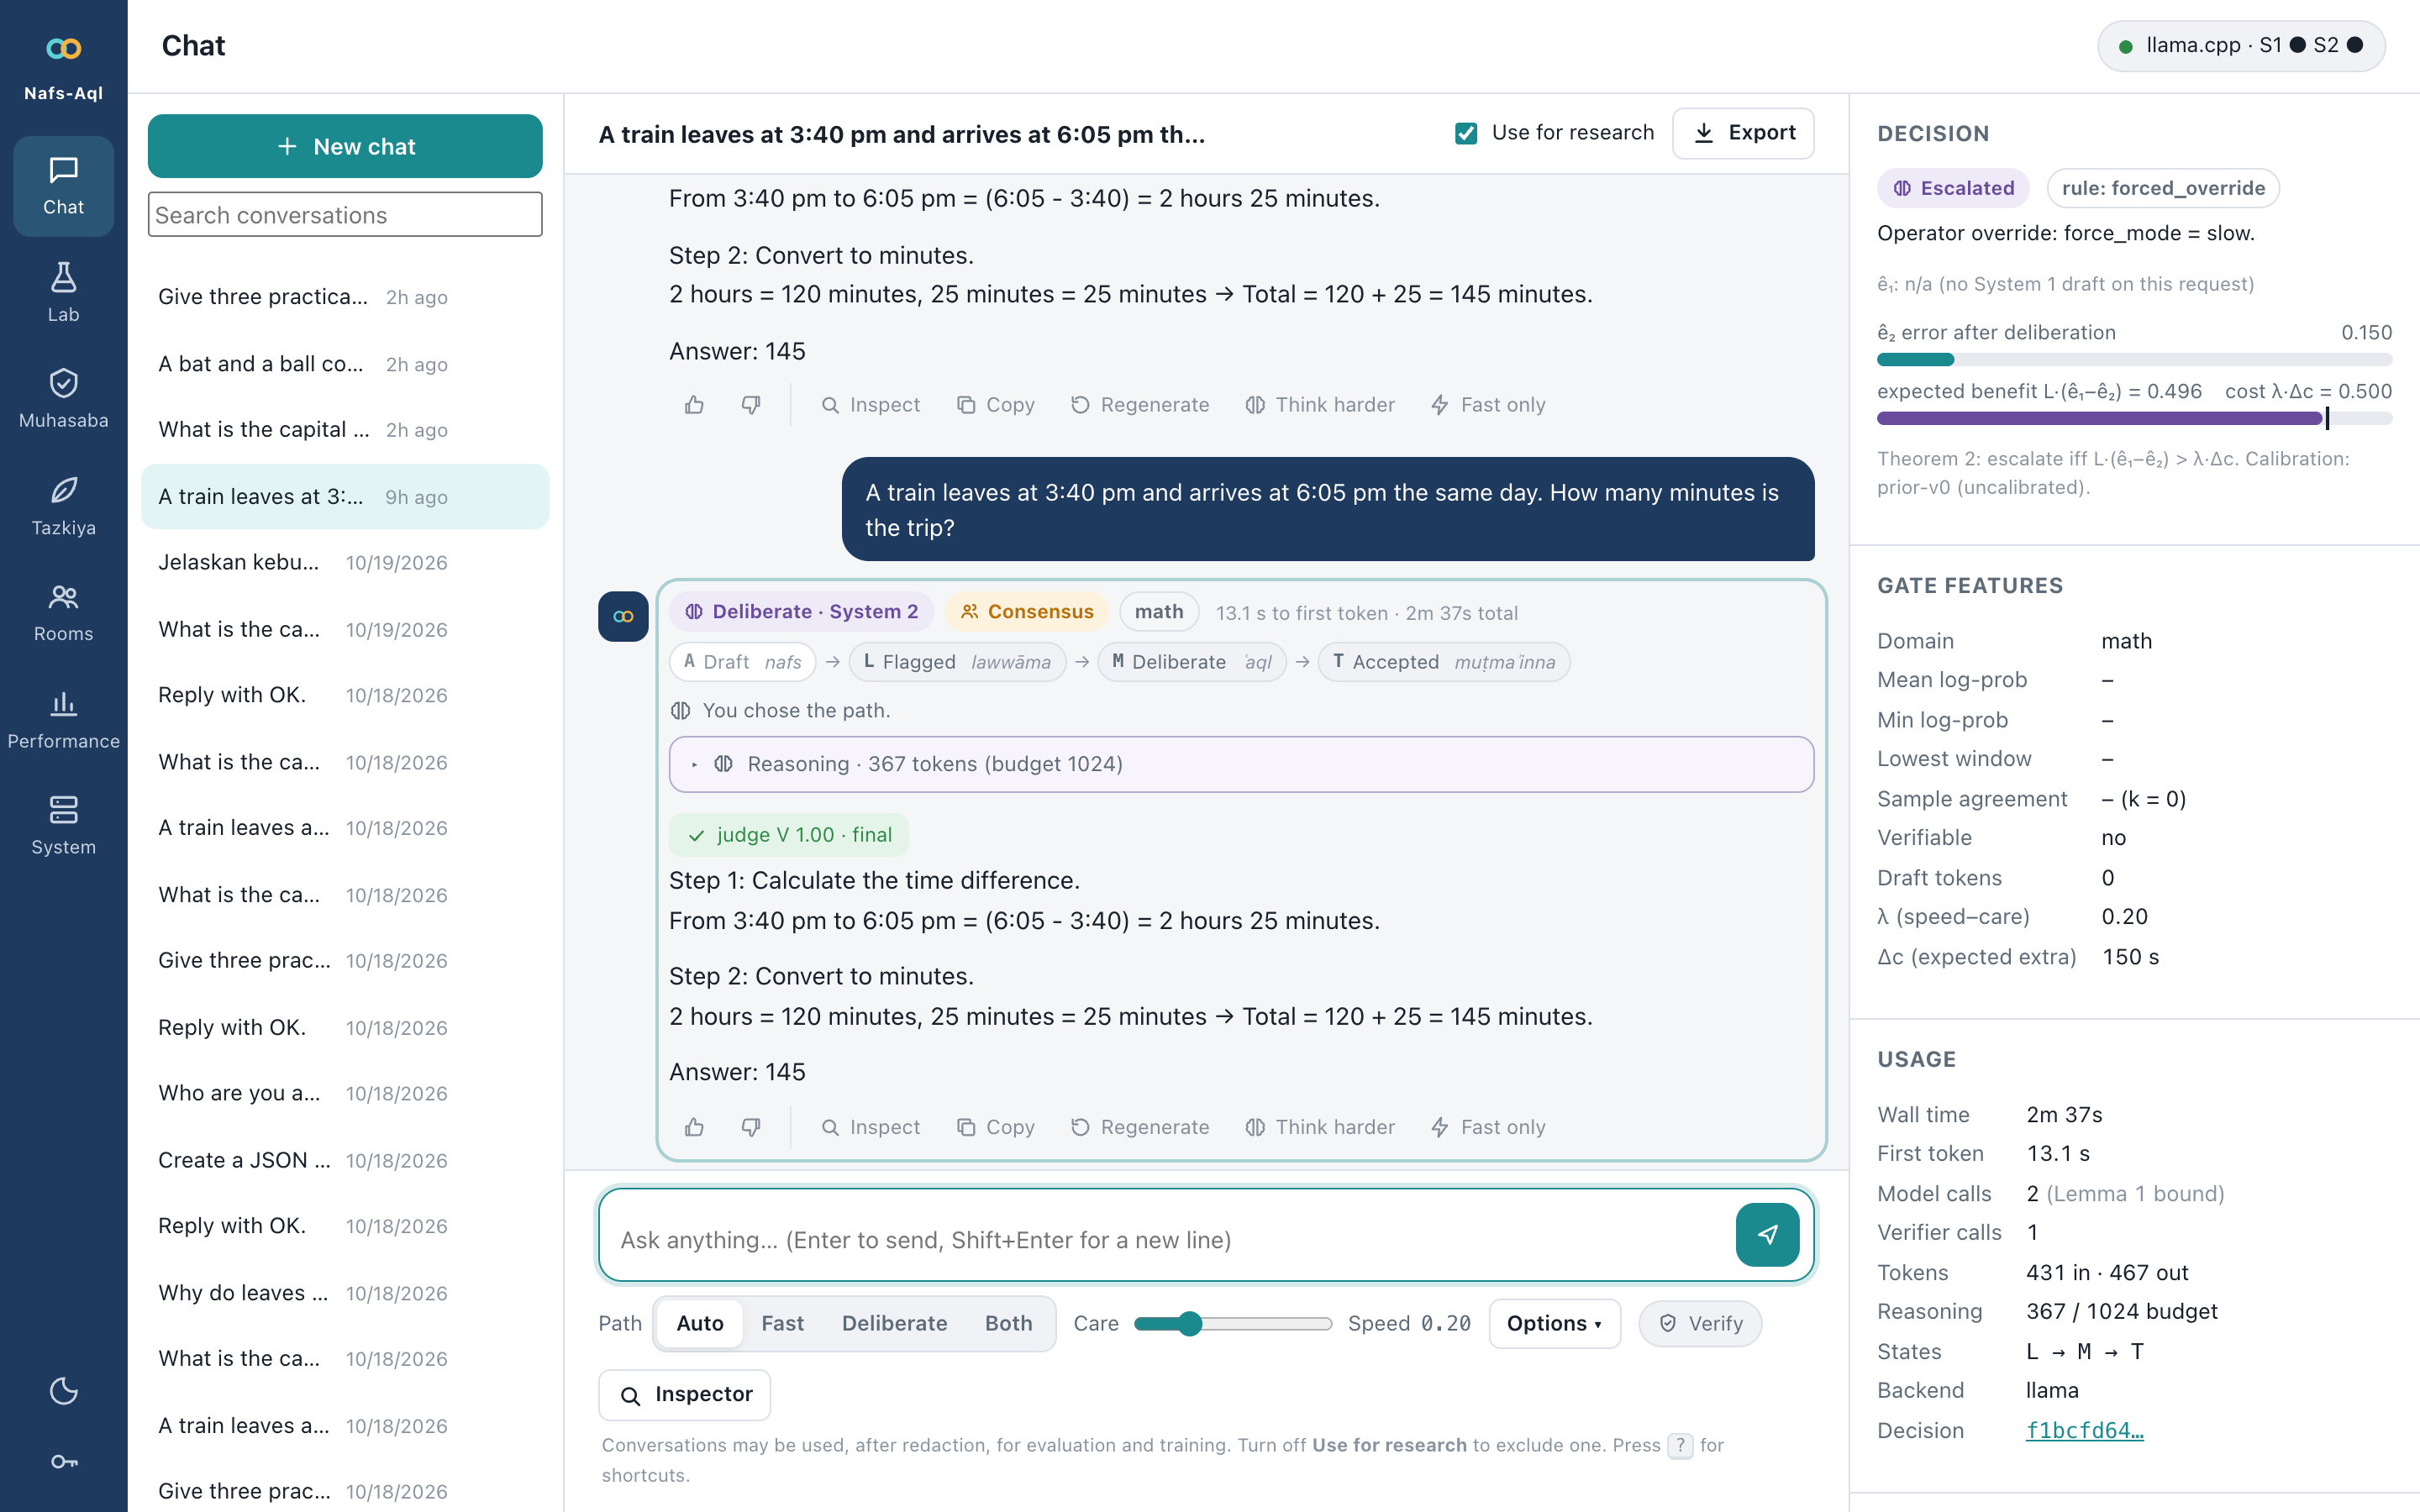
\includegraphics[width=0.9\textwidth]{../shared/screenshots/chat.png}
\caption{Chat page (measured system). A code answer passed the exact verifier on the draft, so the gate kept it
(Theorem~1); the inspector shows the decision, the gate features and the usage.}
\label{fig:ui-chat}
\end{figure*}

\subsection{The laboratory}
The Lab treats each way of combining the two systems as a \emph{policy} and runs them on identical tasks:
\begin{itemize}
\item fast only and deliberate only;
\item the gate with the verifier visible, and the gate routing on its own estimate (``blind'');
\item a draft-conditioned ablation;
\item thinking-budget and $\lambda$ sweeps.
\end{itemize}
Paired differences carry bootstrap intervals, exact McNemar tests and Bonferroni correction. The \emph{policy
map} (Fig.~\ref{fig:ui-lab}) pools every stored run and, for each domain and each price of latency $\lambda$,
names the policy with the lowest expected loss $L(1-\mathrm{acc})+\lambda c$. Over the \PolicyMapRuns{} stored
runs the best policy is, per domain: \PolicyMapSummary. Below a price of about 0.1 per minute of waiting, deliberation
pays for its time on code and mathematics. Above it, the fast path wins, because the verifier already catches most
of its errors.

\begin{figure*}[t]
\centering
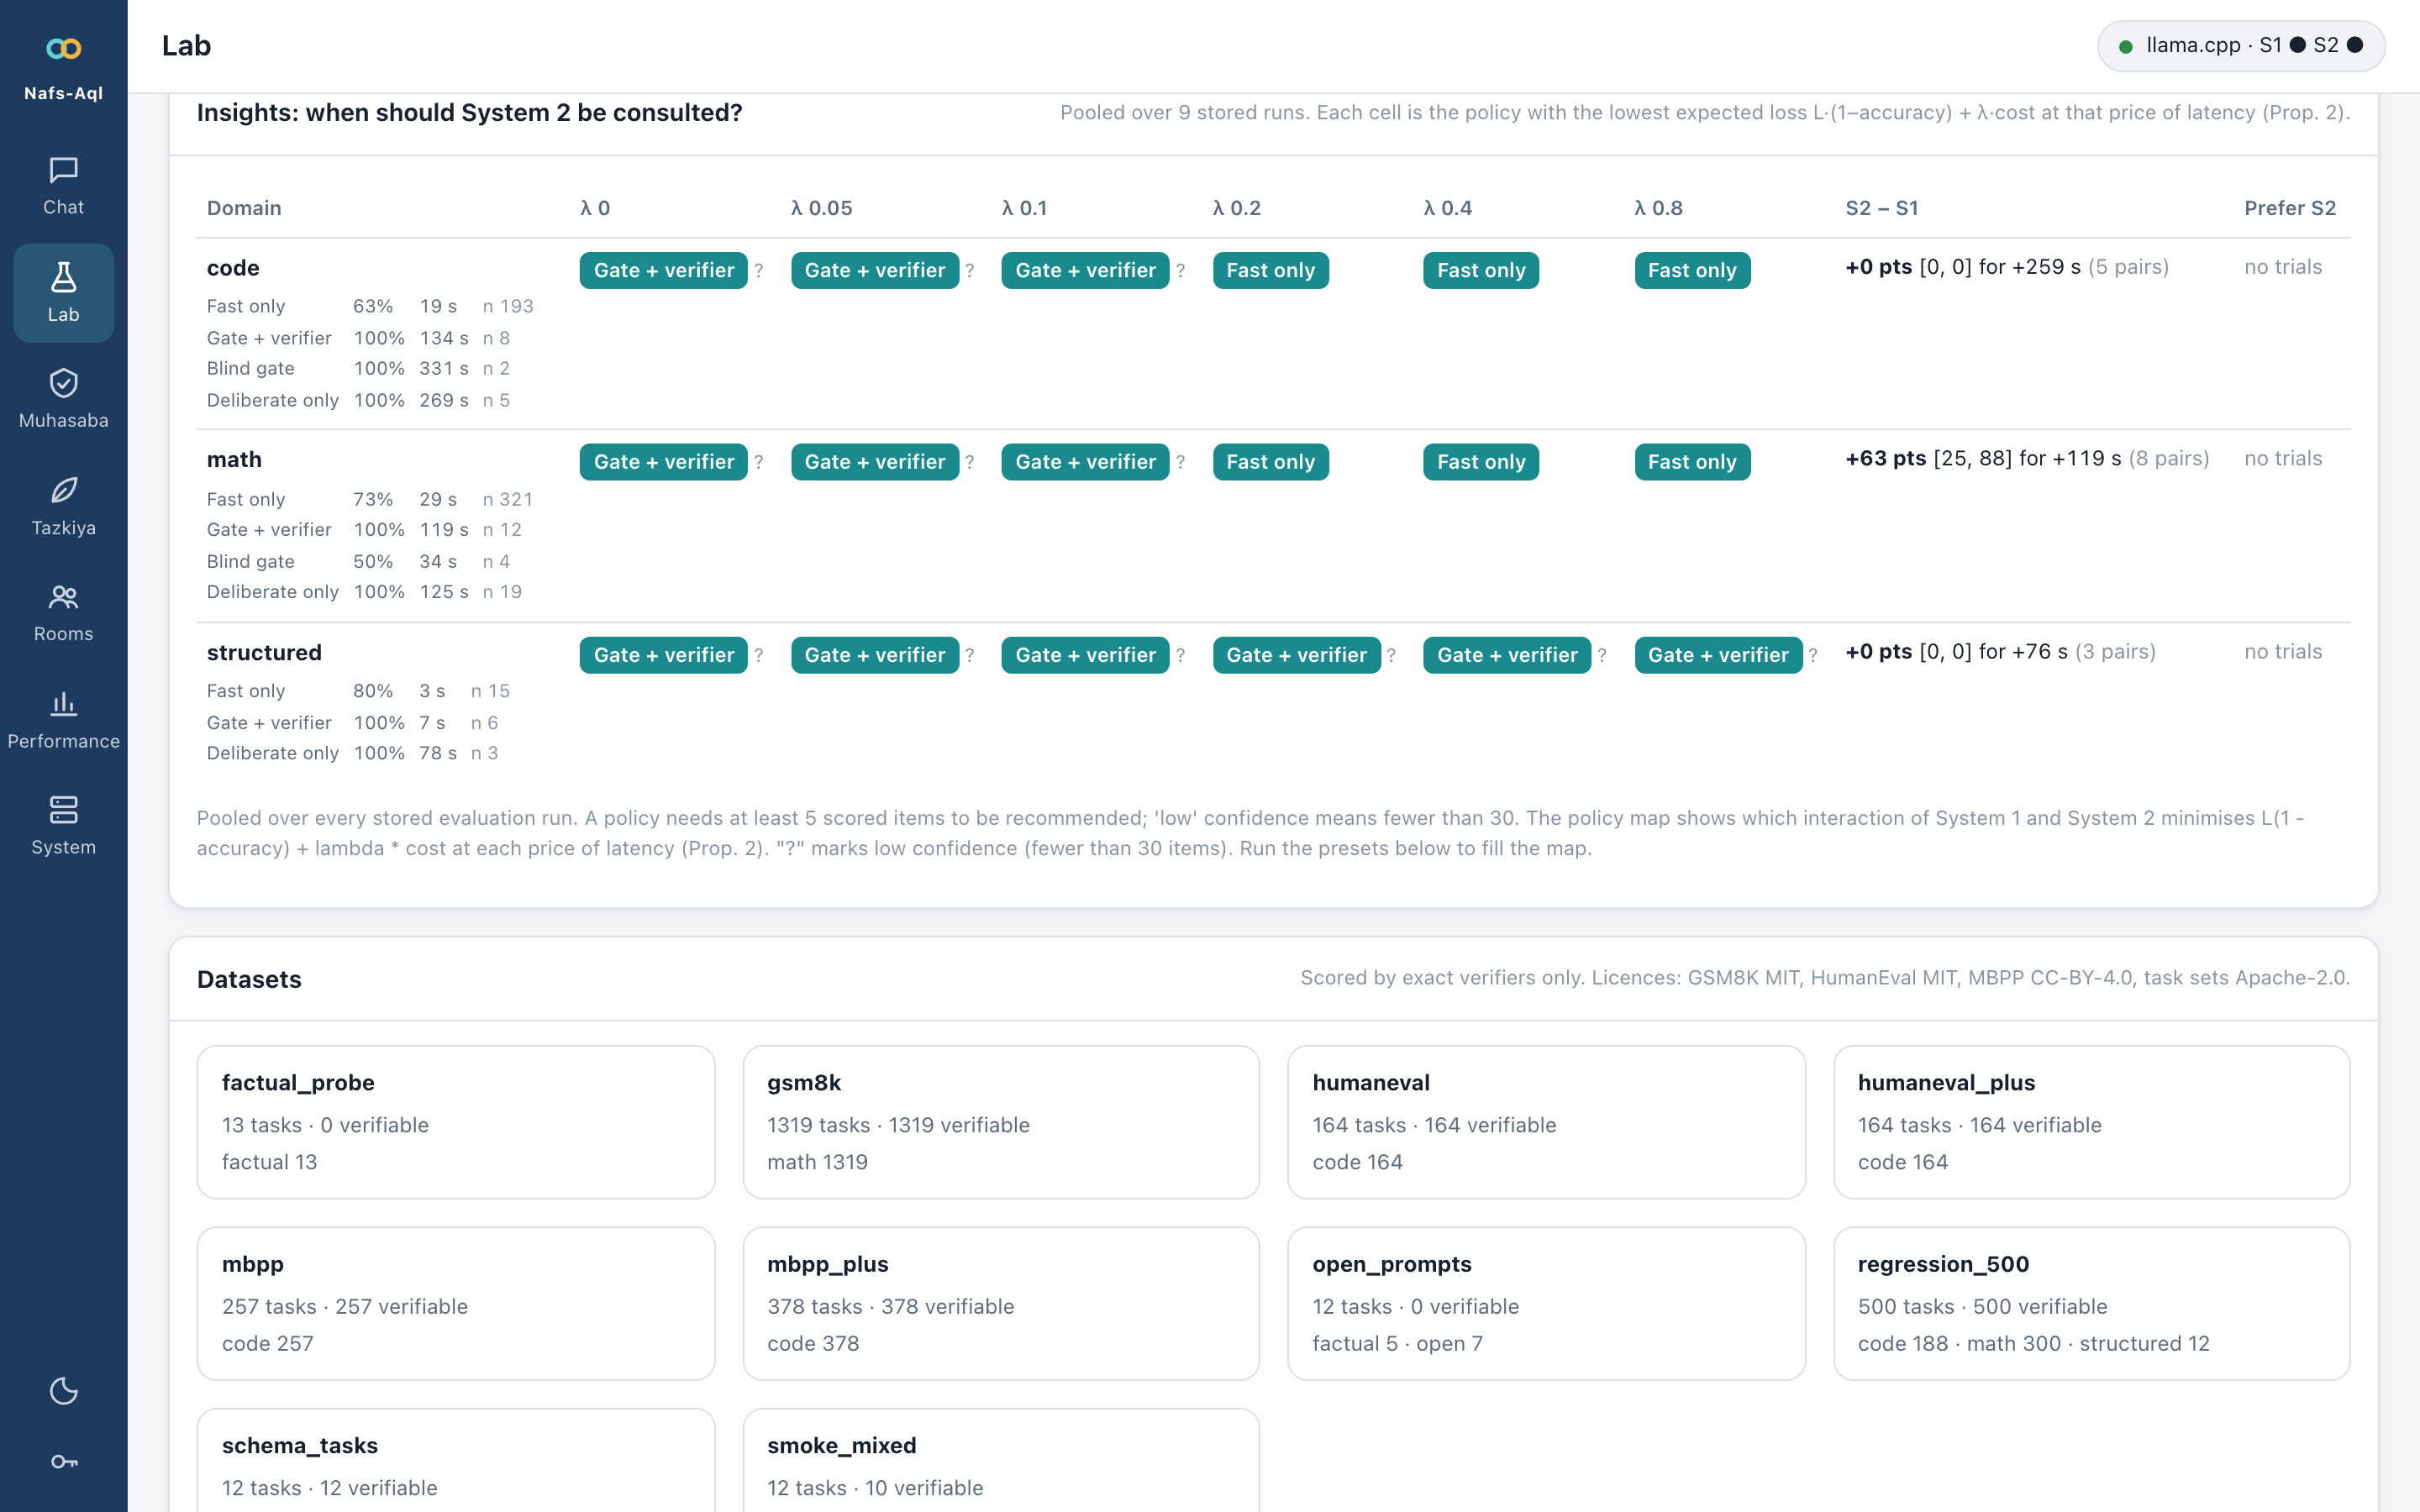
\includegraphics[width=0.48\textwidth]{../shared/screenshots/lab_insights.png}\hfill
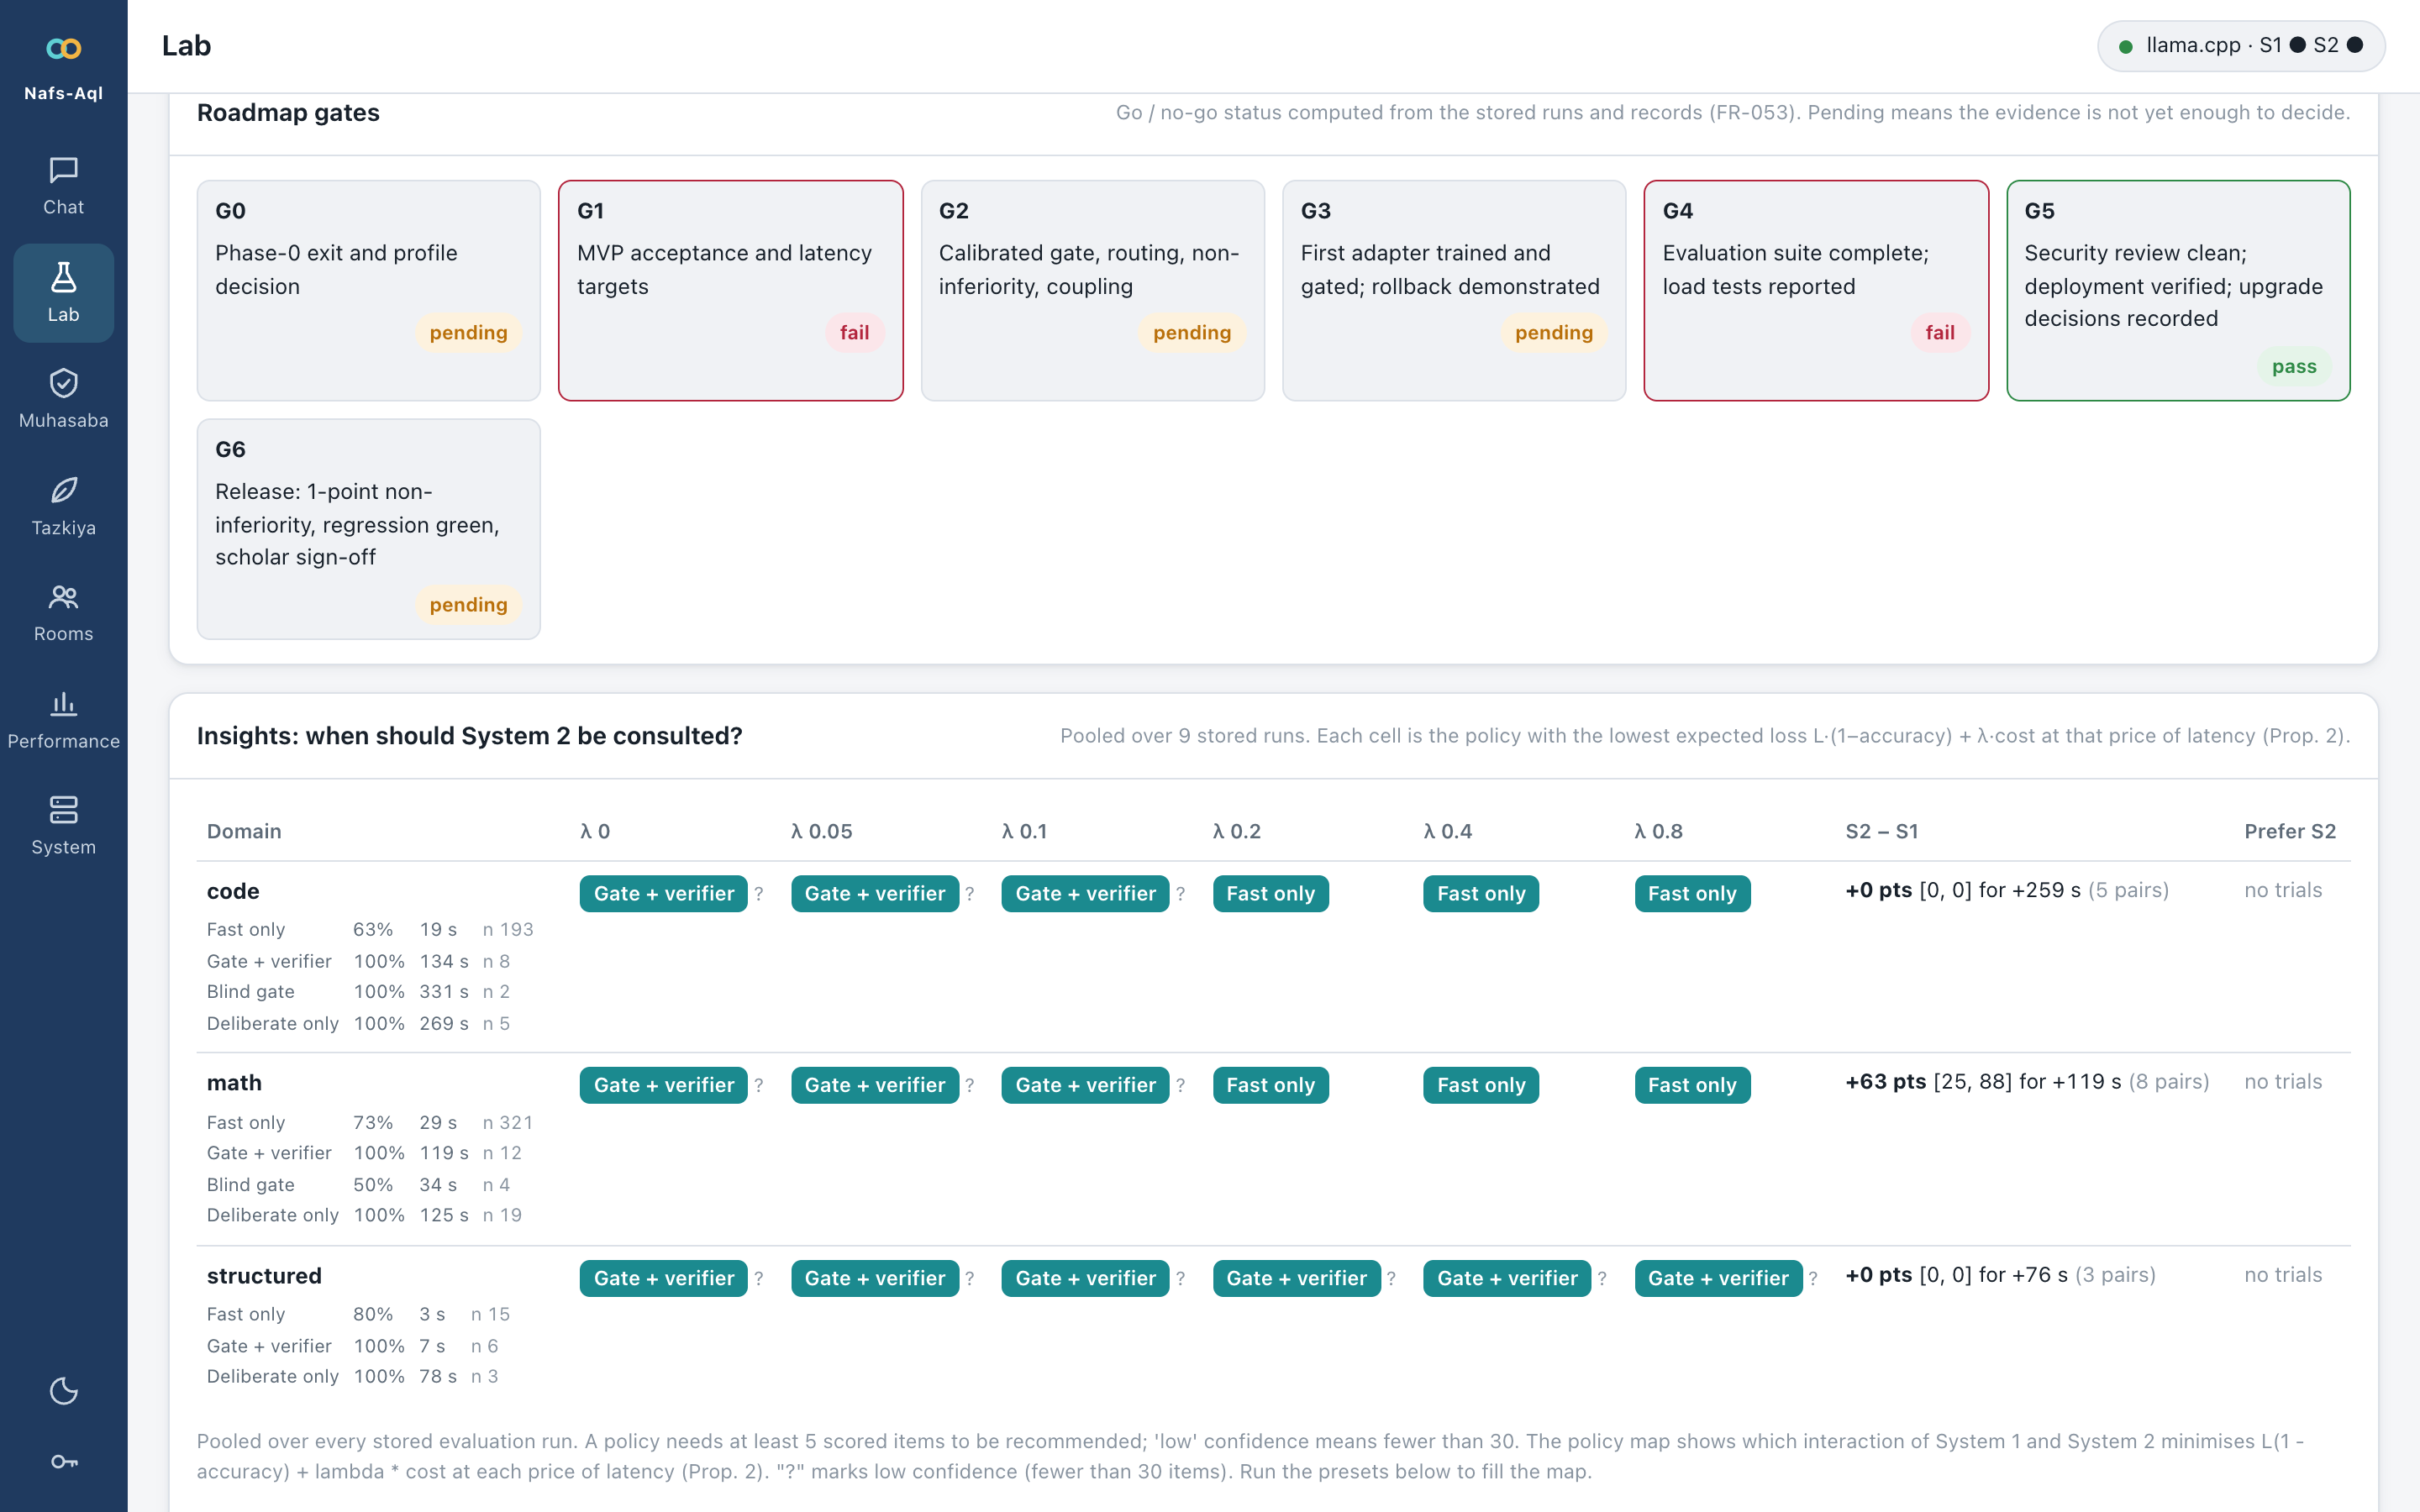
\includegraphics[width=0.48\textwidth]{../shared/screenshots/lab_gates.png}
\caption{Lab page: the pooled policy map, answering ``when should System~2 be consulted?'' per domain and price
of latency (left); roadmap gates G0--G6 evaluated from stored evidence (right).}
\label{fig:ui-lab}
\end{figure*}

\subsection{Policies, verifiers and model choice}
Table~\ref{tab:policies} shows one scaled run of five policies (run \PhaseTwoRun). With the verifier visible,
the gate matched deliberate-only accuracy at \GatedCostRatio{} of its cost. With the verifier hidden, the
uncalibrated gate routed correctly on only \BlindRouting{} of items, because cheap samples agreed with wrong
drafts: agreement is a flag, not evidence (Theorem~\ref{thm:plurality}).

Table~\ref{tab:verifiers} gives the verifiers' measured true- and false-accept rates (runs \RatesRuns).
Mathematics meets the $\varphi\le0.01$ target. The code $\varphi$ is an upper bound inflated by behaviourally
equivalent mutants.

\begin{table}[t]
\centering\caption{Policies on a mixed task set (run \PhaseTwoRun)}\label{tab:policies}
\resizebox{\columnwidth}{!}{\PhaseTwoTable}
\end{table}

\begin{table}[t]
\centering\caption{Verifier quality: $r$ from correct answers, $\varphi$ from seeded mutants}\label{tab:verifiers}
\resizebox{\columnwidth}{!}{\VerifierTable}
\end{table}

The Profile~C decision (MR-005) compared Qwen3.5-2B with Qwen3-1.7B as System~1 on 30 tasks, in alternating
order and with the production prompt (Table~\ref{tab:profilec}). Qwen3.5-2B was more accurate
(\ProfileCDelta), but about 3.7 times slower per task under load. The adoption rule requires latency within
1.3 times, so Profile~A stays the default. The accuracy gain is recorded for a faster host.

\begin{table}[t]
\centering\caption{Profile~C decision (System~1 candidates, 30 tasks)}\label{tab:profilec}
\resizebox{\columnwidth}{!}{\ProfileCTable}
\end{table}

\subsection{CPU inference performance (Phase~7)}
\label{sec:impl:perf}
\textbf{Where the time goes.} Every reply now records its stages:
\begin{itemize}
\item retrieval, the System~1 draft, the cheap samples, verification, System~2 deliberation and the judge;
\item for each model stage, the gateway queue wait and llama-server's own prefill time, decode time and
KV-cache reuse.
\end{itemize}
Over \StageReplies{} replies with stage timings, the fast path spends essentially all of its time in the System~1
draft, and the deliberate path in System~2 deliberation (Table~\ref{tab:stages}, Fig.~\ref{fig:ui-perf}); verification and gating are negligible. The prompt cache already serves most prompt tokens
(Table~\ref{tab:engine}), so prefill is small. \emph{Decode speed is the bottleneck}, and it falls several-fold
when other workloads share the four cores: 2.6--4.3 tokens/s in service, against 22.9 in an idle llama-bench run.

\begin{table}[t]
\centering\caption{Latency by stage (share of wall time)}\label{tab:stages}
\resizebox{\columnwidth}{!}{\StageTable}
\end{table}
\begin{table}[t]
\centering\caption{Engine speed per model stage (llama-server timings)}\label{tab:engine}
\resizebox{\columnwidth}{!}{\EngineTable}
\end{table}

\begin{figure*}[t]
\centering
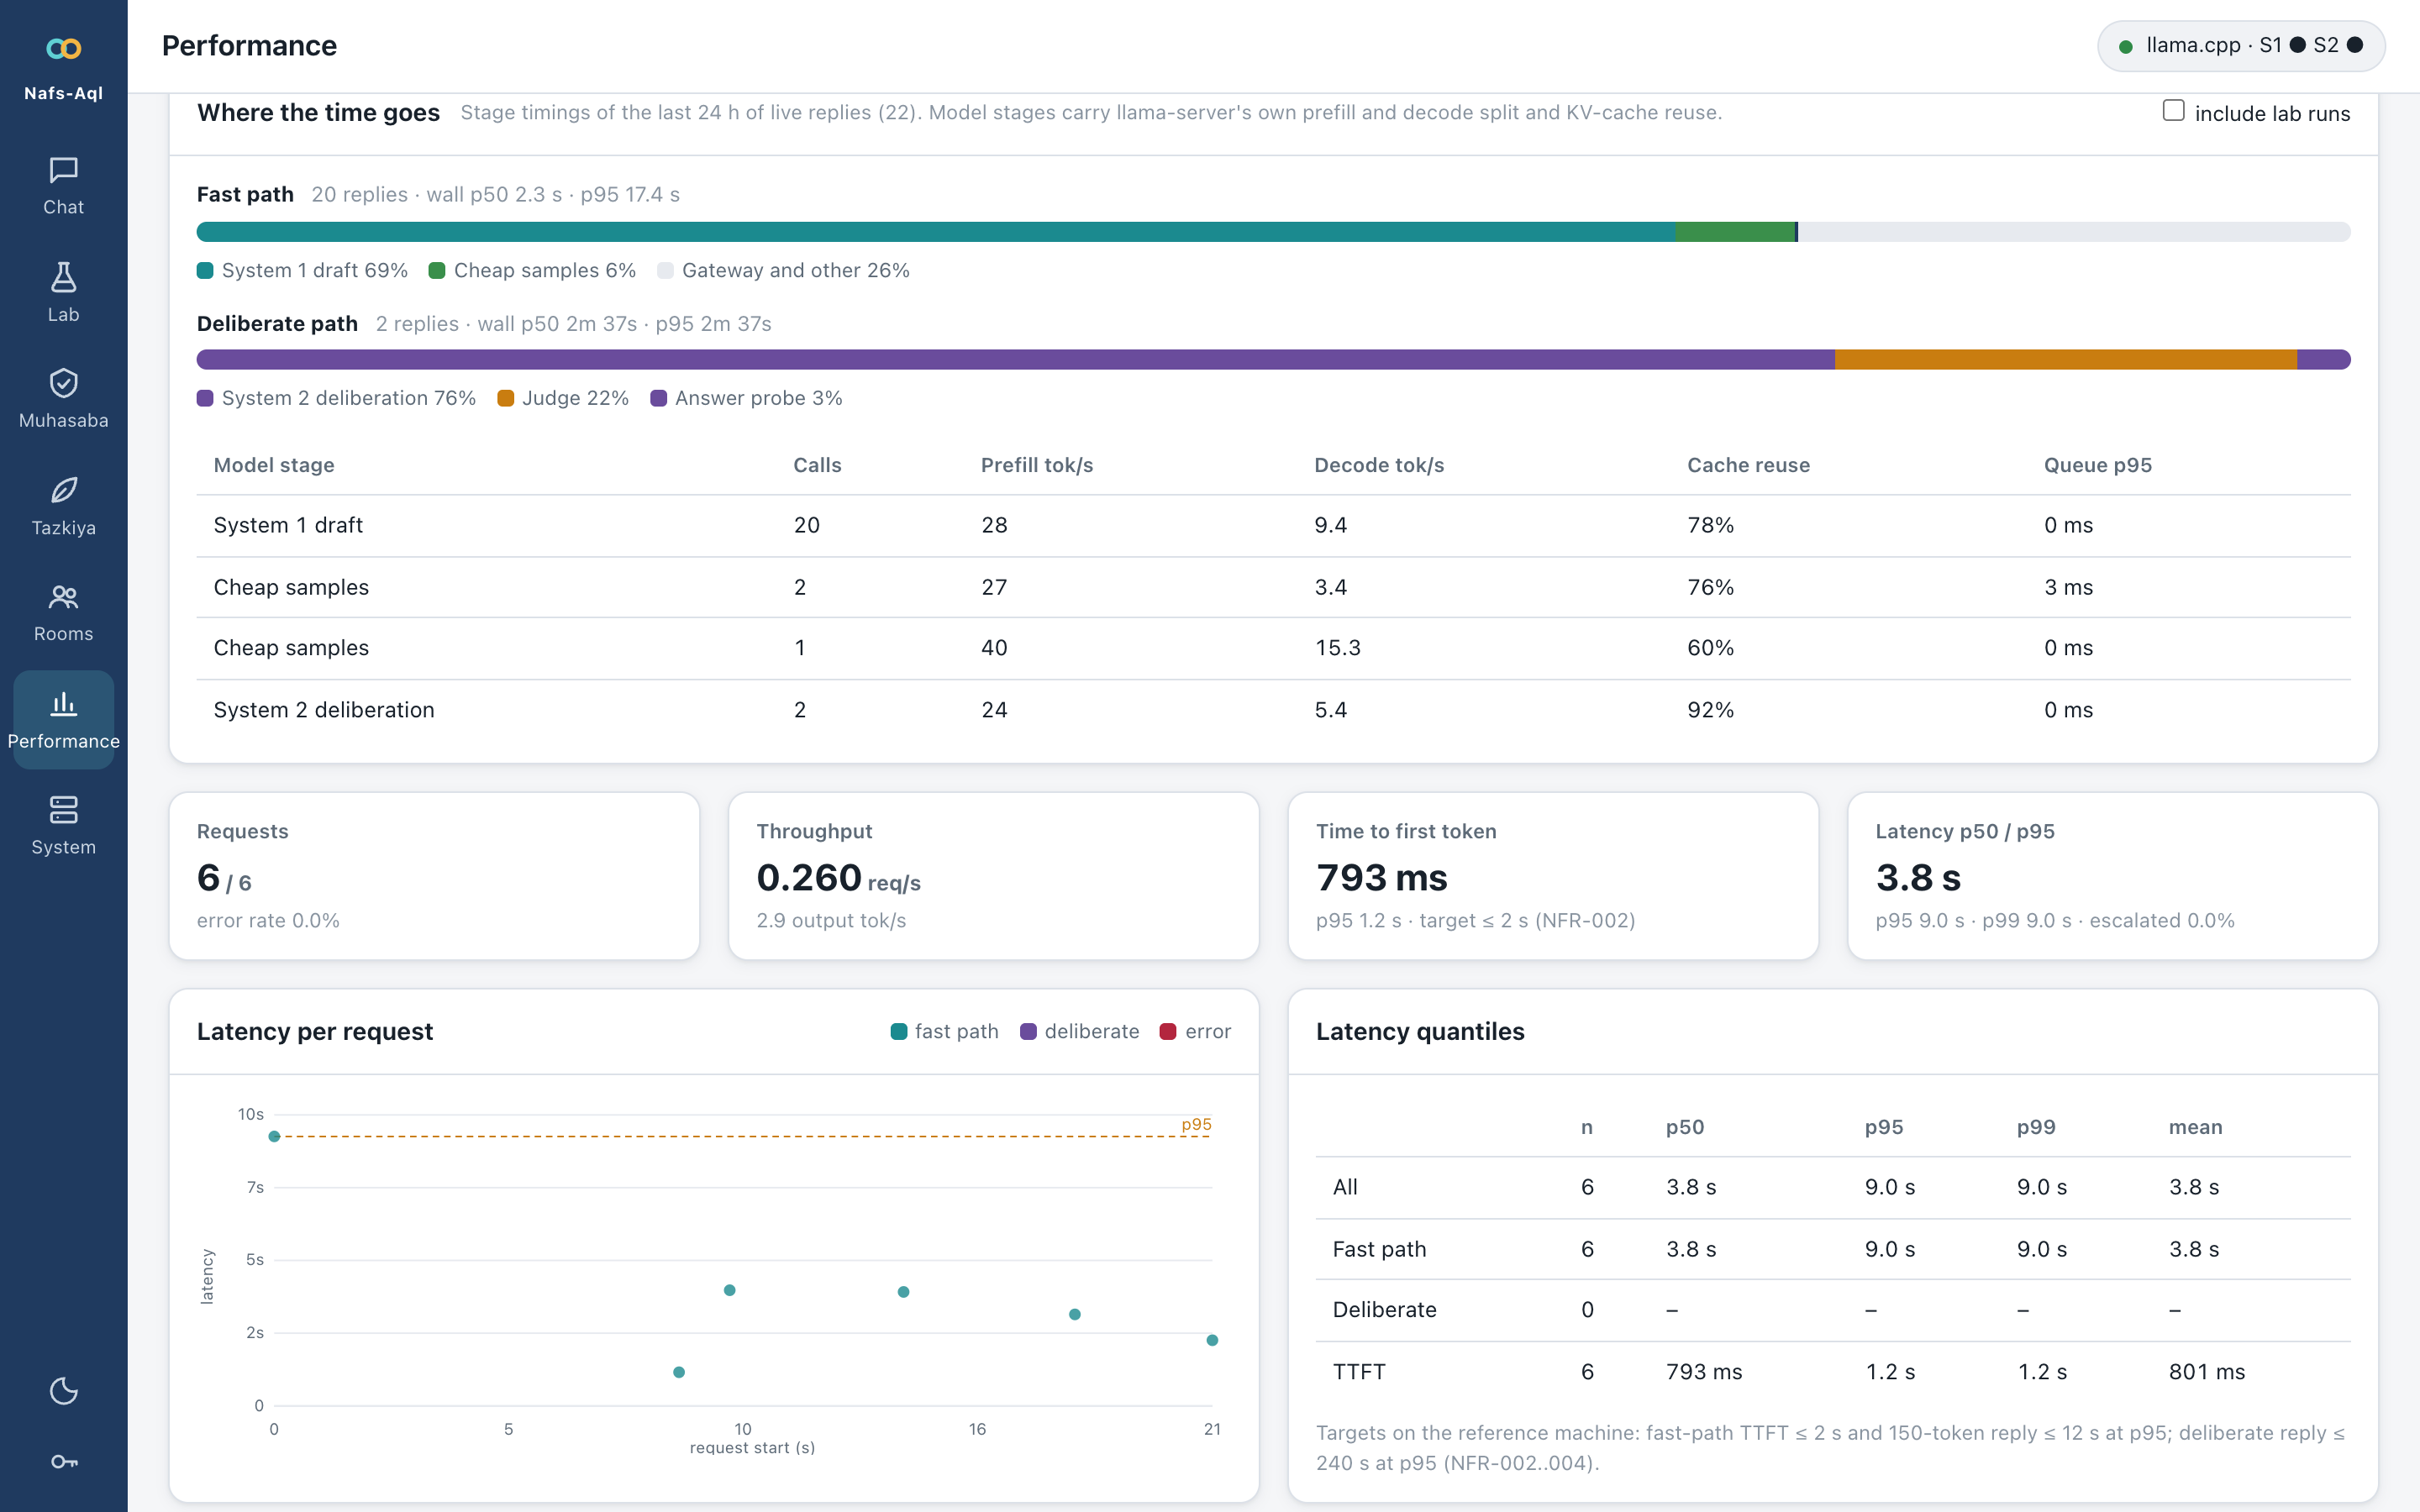
\includegraphics[width=0.48\textwidth]{../shared/screenshots/performance_stages.png}\hfill
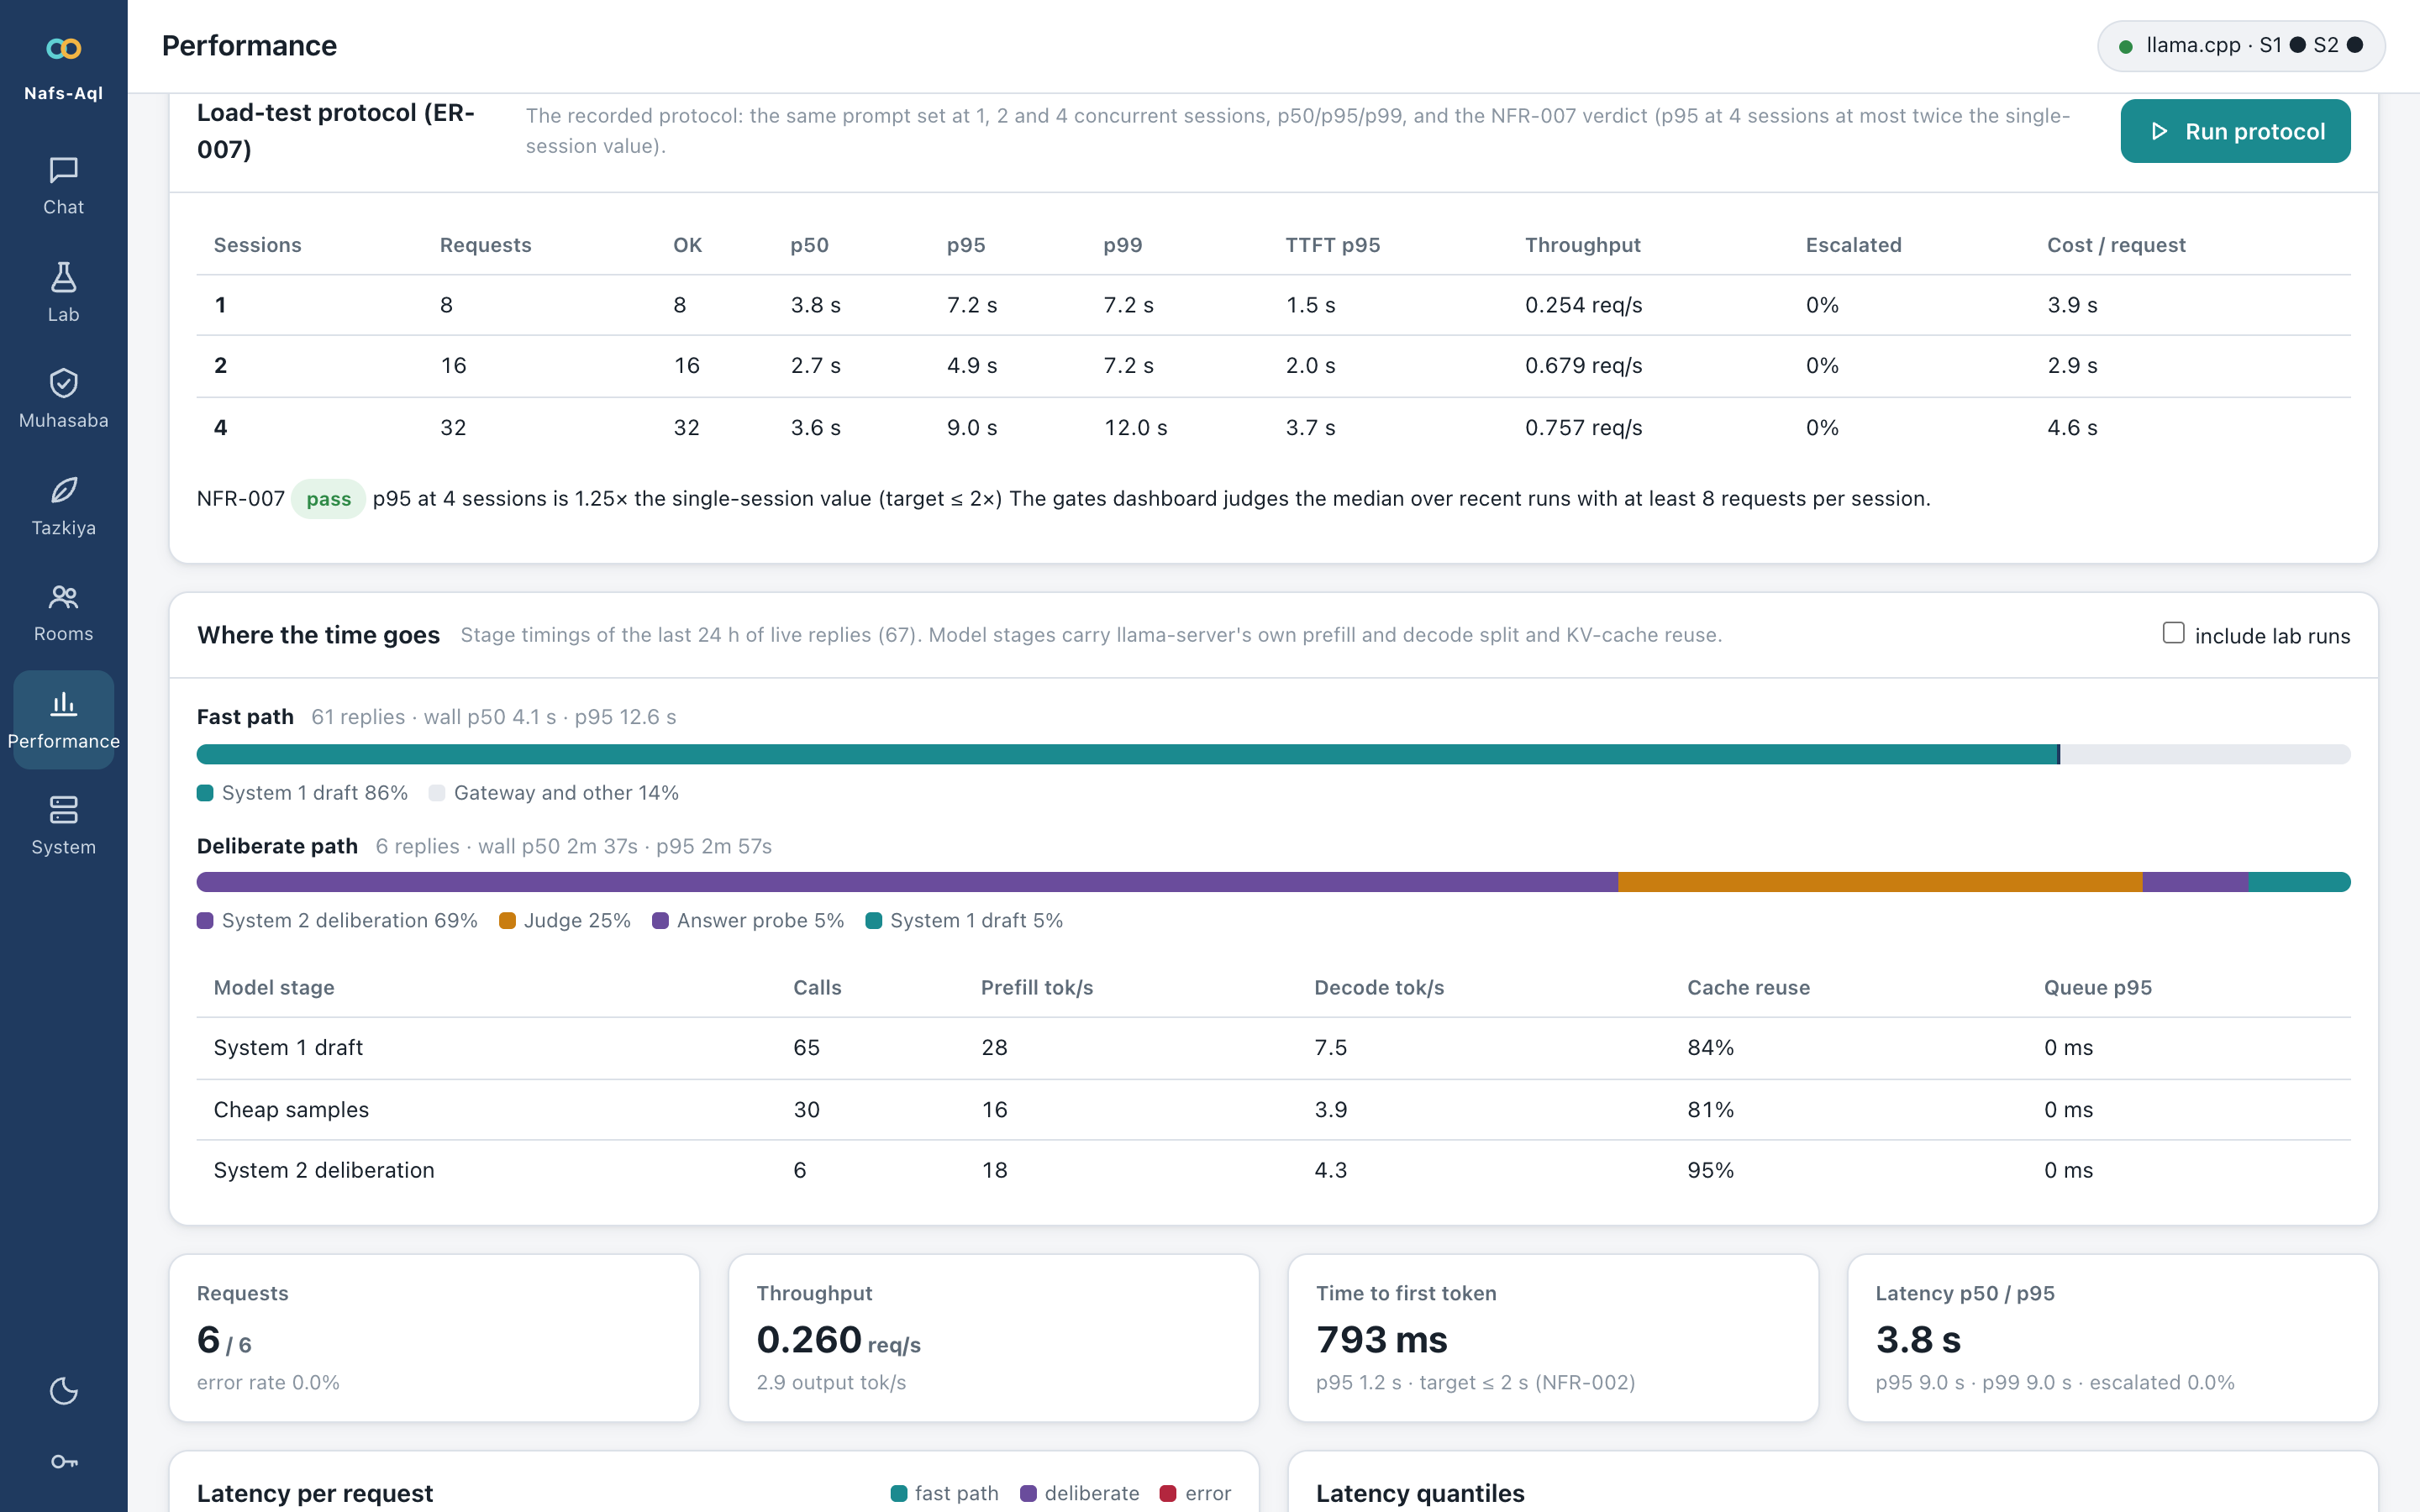
\includegraphics[width=0.48\textwidth]{../shared/screenshots/performance.png}
\caption{Performance page: where the time goes, from stage timings, with the engine's prefill and decode speed
and cache reuse (left); the load-test protocol at 1, 2 and 4 sessions with the NFR-007 verdict (right).}
\label{fig:ui-perf}
\end{figure*}

\textbf{Techniques and their measured effect.} Each change was accepted only after an interleaved A/B on the
reference machine (NFR-031):
\begin{itemize}
\item \emph{Skipping cheap samples when an exact verifier decides} (Theorem~1 makes them irrelevant): median
draft time fell from 13.4\,s to 7.9\,s.
\item \emph{Prompt-cache warm-up} at start-up, with llama-server's host-memory prompt cache: a cold first request
had 9.8\,s time to first token, a warm one about 1\,s.
\item \emph{Verifier warm-up}: the first verification after start-up fell from 0.45\,s to 3\,ms.
\item \emph{Early escalation} (FR-080): under the fixed rule, an open-ended draft whose running mean log-prob is
already below the threshold minus a margin is stopped and handed to System~2, instead of being generated to the
end, in the spirit of cost-aware cascades \cite{chen2023frugalgpt,yue2024cascades}. In the agreement study, \EarlyEscSummary{} (Table~\ref{tab:early}).
\item \emph{Sequential, uncertainty-gated samples}: the two agreement samples had run concurrently with
the draft, and three sequences on four cores tripled the factual fast path (12.6\,s median, 1.4\,s to first
token). They are now drawn after the draft and only when its mean log-prob lies within 0.10 of the threshold;
the path is 4.3\,s and 0.14\,s, the same as drawing no samples.
\item \emph{Four System~1 slots}: four sessions no longer queue behind three; batched decode makes the fourth
slot cheap.
\item \emph{No gain}, so not adopted:
  \begin{itemize}
  \item speculative decoding \cite{leviathan2023speculative} with a 0.6B draft model (6.5 against 7.3 tokens/s), because the draft model
  competes for the same cores and memory bandwidth;
  \item n-gram lookup;
  \item flash attention and a q8\_0 KV cache: a sequential run suggested a 30\% gain, which an interleaved repeat
  showed to be an ordering effect of the shared load.
  \end{itemize}
\end{itemize}

\begin{table}[t]
\centering\caption{Early-escalation agreement study (open-ended prompts)}\label{tab:early}
\EarlyEscTable
\end{table}

\textbf{Concurrency.} The load-test protocol (latest run \ProtocolRun, Table~\ref{tab:protocol}) gave a 4-session
p95 of \NfrSevenRatio{} times the single-session value. The gate judges NFR-007 on the median over recent eligible
runs (\NfrSevenPooled), because single runs on the shared host ranged from 1.25 to 2.48.

\begin{table}[t]
\centering\caption{Load-test protocol, fast path (run \ProtocolRun)}\label{tab:protocol}
\ProtocolTable
\end{table}

\textbf{Adaptive reasoning exit (FR-082).} The deliberate path is almost entirely System~2 reasoning, so the
second Phase~7 change shortens the reasoning itself, in the spirit of the 2026 early-exit methods
(DTSR, DEER, Dynasor-CoT) but with the design's own stopping signal. System~2 reasons in chunks on
llama-server's raw continuation endpoint, which keeps the prefix cached. At a reflection signal (``Wait'',
``Alternatively'', \ldots), with a minimum gap of 64 tokens and at the latest every 256 tokens, the reasoning
is closed provisionally and the model is asked for its answer in a few tokens. On a verifiable task the exact
verifier judges that probe and, if it passes, the reasoning stops; on factual tasks two consecutive agreeing
probes stop it. The final answer is then generated after the reasoning exactly as on the standard path, so the
exit changes only how much reasoning is generated, and the exit reason is recorded with the reply. A probe
costs 0.6--0.8\,s. In the paired Lab comparison (run \AdaptiveExitRun), \AdaptiveExitSummary.

\textbf{EAGLE-3 speculative heads} \cite{li2024eagle} for both models (AngelSlim, Apache-2.0) were converted and
measured in interleaved A/B runs (Table~\ref{tab:eagle}). On a GPU these heads give 1.7$\times$ because
verifying a draft is nearly free there. On four cores the verification pass costs real compute, and at the
measured acceptance of about half the drafted tokens neither system gained: System~1 1.04$\times$ greedy and
0.95$\times$ at the production temperature, System~2 0.99$\times$ on reasoning prompts; eight draft tokens were
slower than no speculation on both. The heads stay available
as an opt-in (\texttt{EAGLE=1}) for a host with more cores. Weight formats with AVX2 repack kernels
(Q4\_0, IQ4\_NL) remain to be measured the same way.

\begin{table}[t]
\centering\caption{EAGLE-3 speculative decoding, interleaved A/B on the reference CPU}\label{tab:eagle}
\resizebox{\columnwidth}{!}{\EagleTable}
\end{table}

\textbf{Weight formats.} Q4\_0 and IQ4\_NL use llama.cpp's AVX2 repack kernels, which read the weights in an
interleaved layout; Table~\ref{tab:quant} compares them with the production Q4\_K\_M on the same model
(interleaved \texttt{llama-bench} runs, 4 threads, host load recorded in the log).
\begin{table}[t]
\centering\caption{Weight formats, Qwen3-1.7B, llama-bench pp128/tg64}\label{tab:quant}
\QuantTable
\end{table}

\textbf{A smaller judge?} The rubric judge is the largest fixed cost on open questions once the adaptive exit
is in place (26--40\,s per answer on System~2). Scoring with System~1 instead would be about three times
faster, so it was measured with the rates harness on the same labelled items: \JudgeCompare. A judge that
accepts a quarter of the seeded wrong answers is not a soft verifier in the sense of Theorem~1, so the judge stays
on System~2; the backend remains a configuration option for hosts with a larger small model.

\textbf{vLLM backend.} The second serving profile, vLLM's CPU backend, now runs in Docker from the team's
\texttt{carstenz/vllm-smoke} image (vLLM 0.30, x86 CPU build) with Qwen3-1.7B serving both roles from the host's
Hugging Face weights, and the gateway switches between the two backend sets at run time. Two facts shaped the
recipe. First, the Docker VM exposes AVX2 only, where oneDNN has no BF16 kernels: in BF16 the engine loaded but
never returned a token, so the model runs in FP32 (6.8\,GB of weights). Second, the VM's memory cap matters: at
6\,GiB only 0.18\,GiB remained for the KV cache and at 10\,GiB with a 2\,048-token context the engine was OOM-killed
during its profiling pass, so the context, the prefill batch and the KV cache are kept small. The gateway-side
check, which drives every request path the orchestrator depends on against the backend, reports
\VllmCheckSummary. On four shared cores the three-vCPU VM is a correctness and portability profile, not a
speed contest with llama-server.

\subsection{Operations and the gates}
Monitoring and safety:
\begin{itemize}
\item \textbf{Drift and alerts} (Fig.~\ref{fig:ui-muh}): a two-sided CUSUM per domain on calibration error and
fast-path accuracy, with a shuffled negative control. Five alert rules run over live traffic only; evaluation
and load-test replies are tagged as lab traffic.
\item \textbf{Security:} \SecuritySummary. The suite found one high-severity issue, now fixed: sandboxed code
could signal other processes.
\item \textbf{Deployment checks:} \DeploySummary.
\end{itemize}
Table~\ref{tab:gates} lists the roadmap gates as evaluated from stored evidence. The gates that remain pending
need release-scale runs (thousands of paired items), GPU training, or the scholar review of the analogy text.

\begin{figure*}[t]
\centering
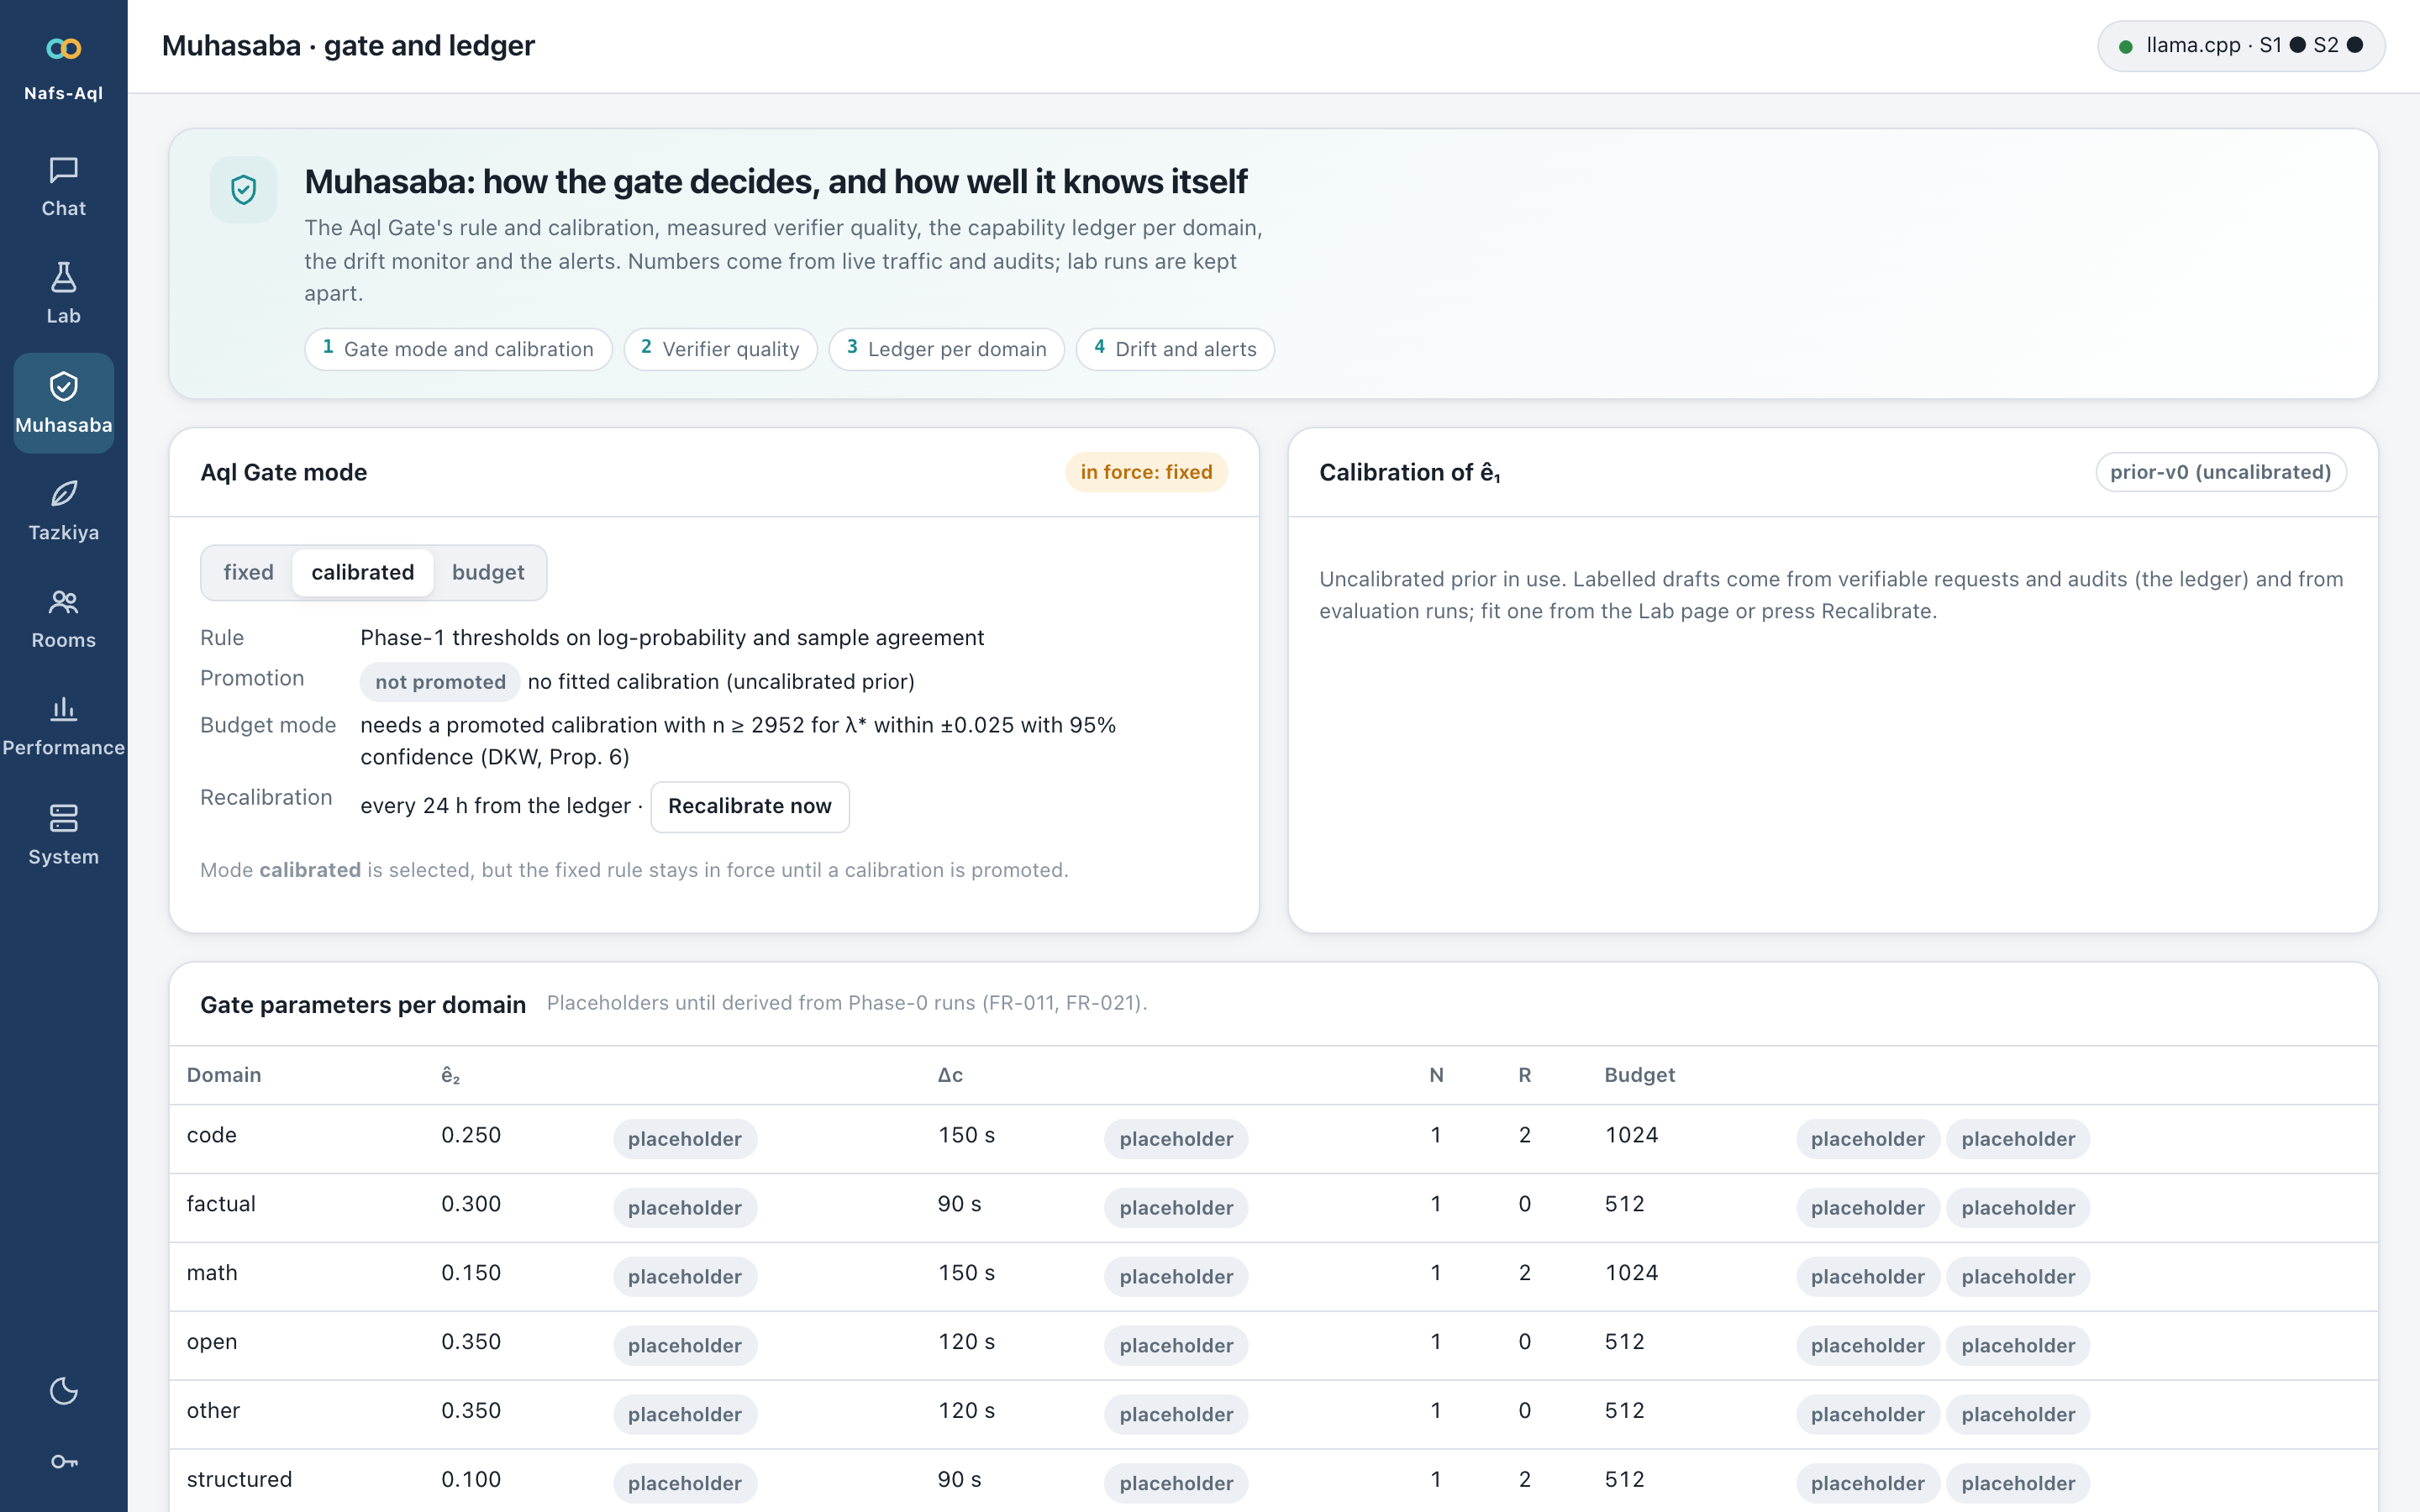
\includegraphics[width=0.48\textwidth]{../shared/screenshots/muhasaba.png}\hfill
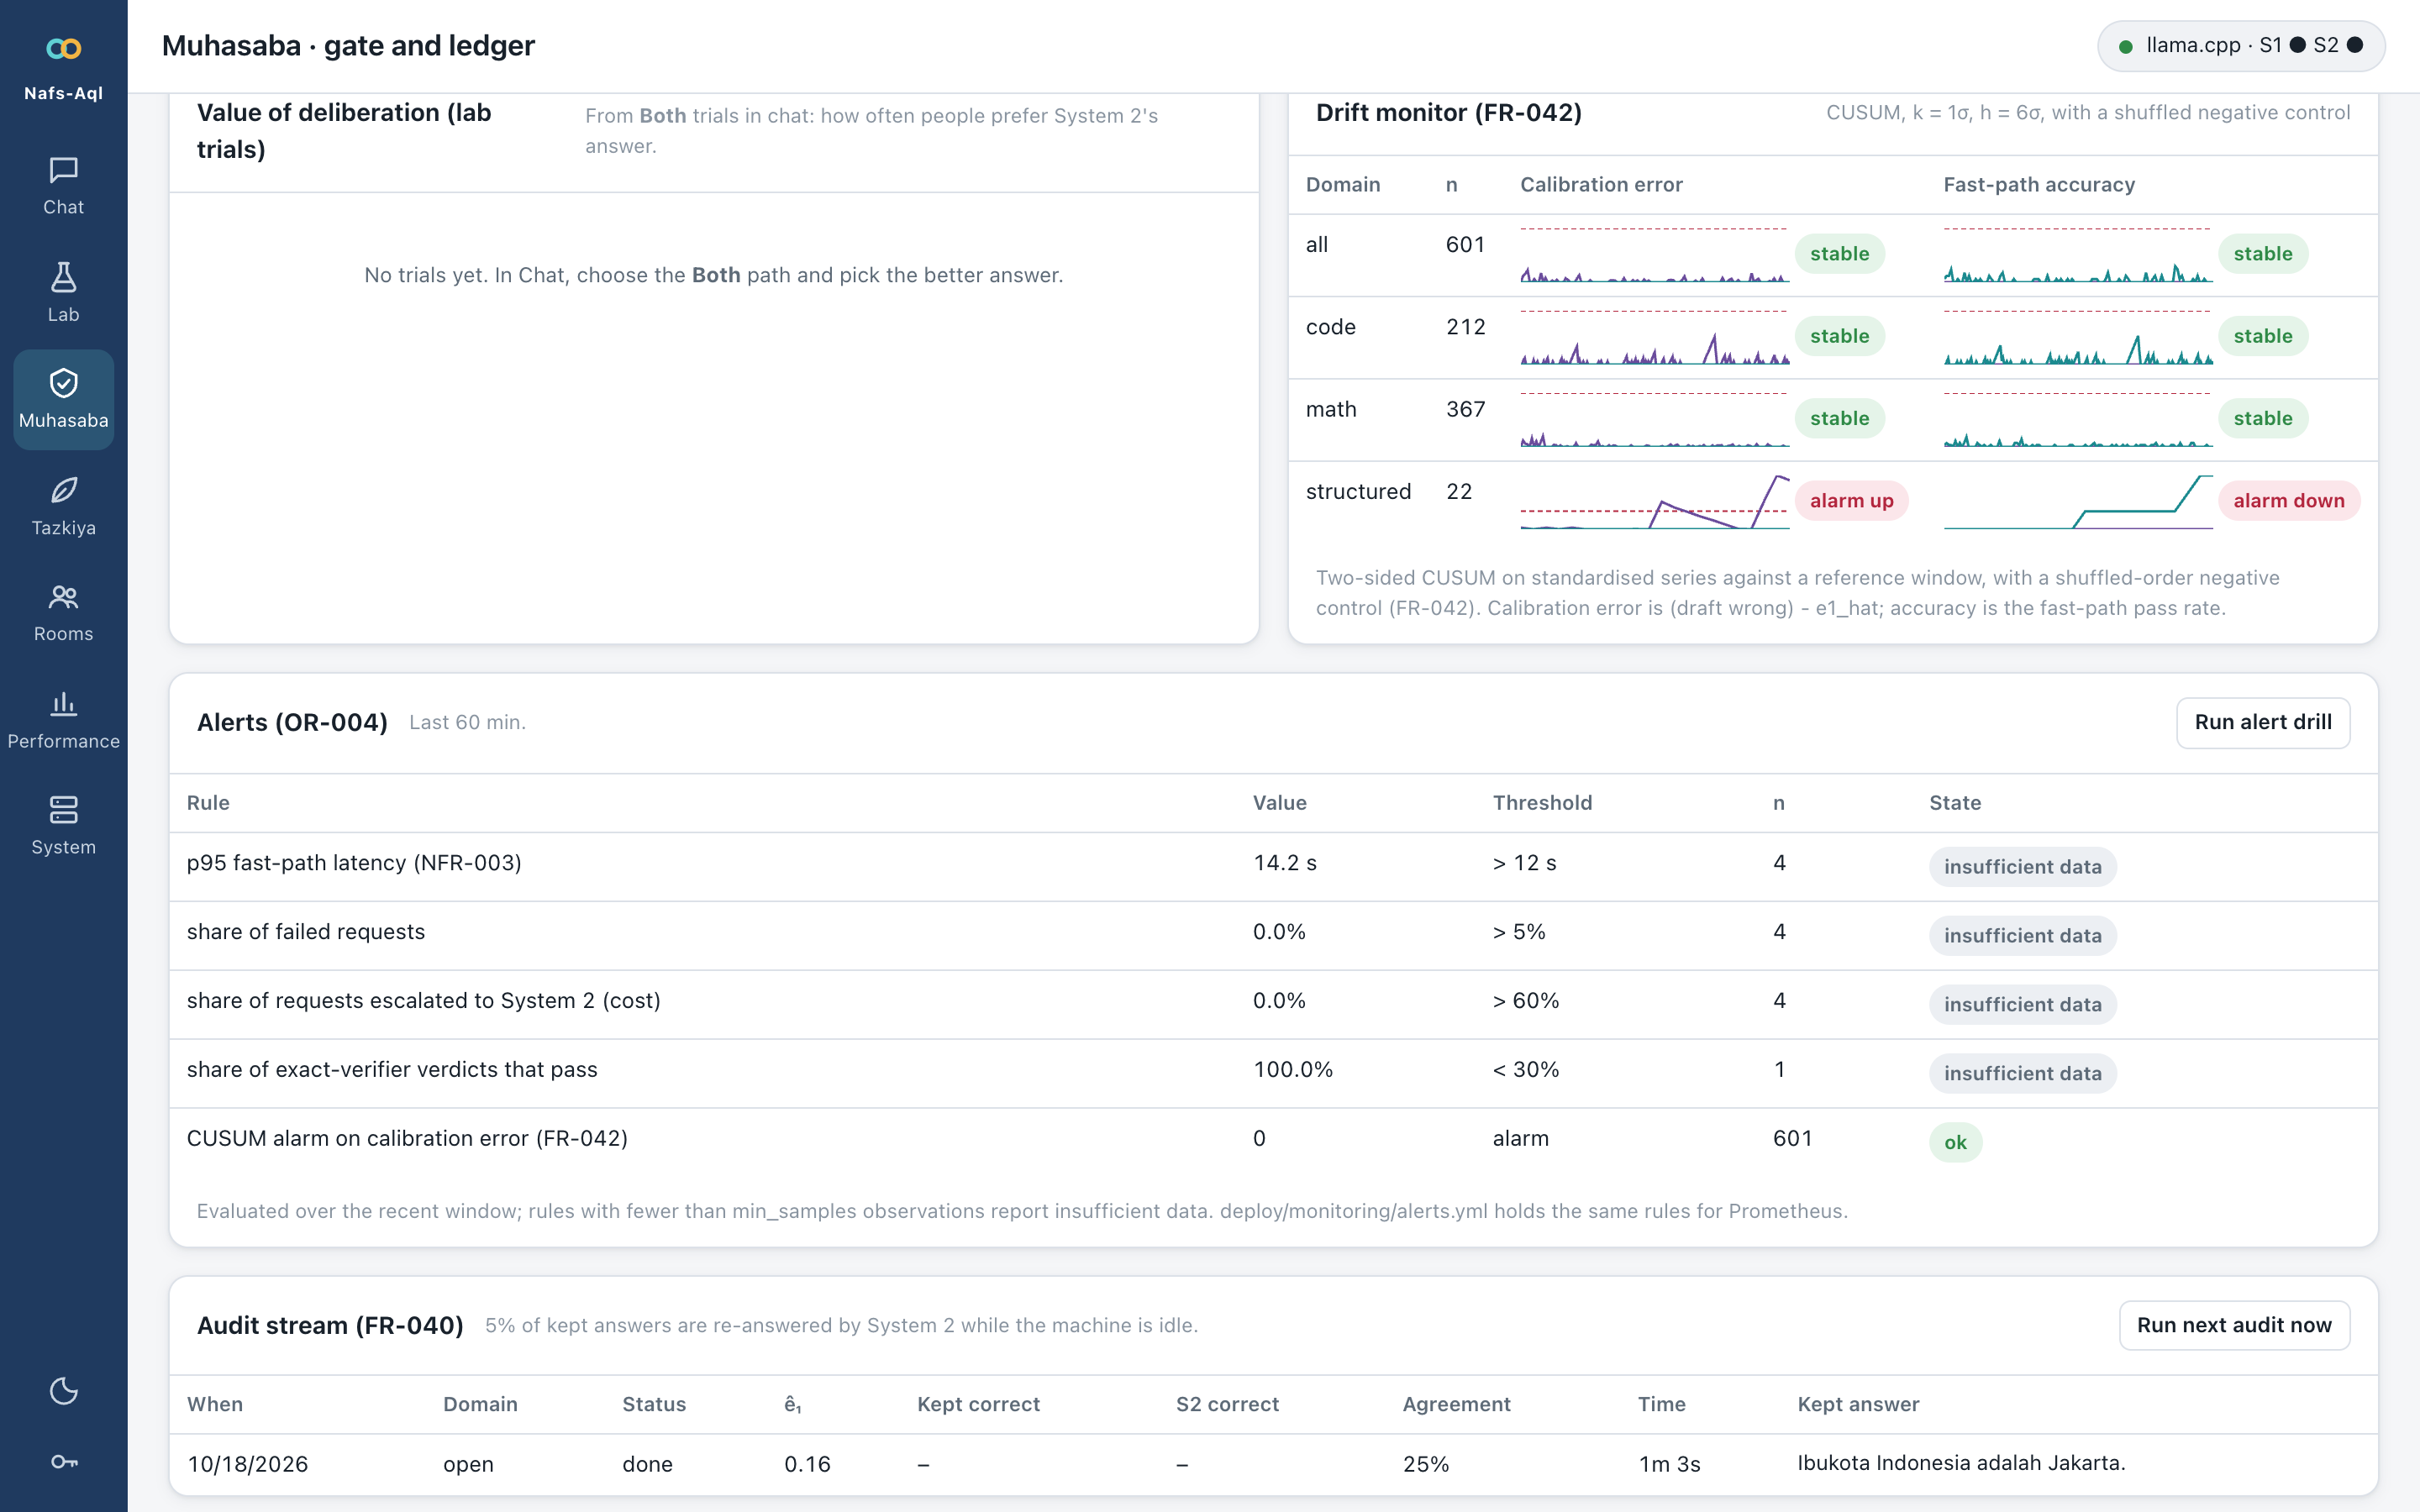
\includegraphics[width=0.48\textwidth]{../shared/screenshots/muhasaba_drift_alerts.png}
\caption{Muhasaba page: gate mode, promotion status and calibration (left); drift monitor and alert rules over
live traffic (right).}
\label{fig:ui-muh}
\end{figure*}

\begin{table*}[t]
\centering\caption{Roadmap gates evaluated from stored evidence (18 October 2026)}\label{tab:gates}
\small\GatesTable
\end{table*}

% ---------------------------------------------------------------------------
% Section: Phase 8 -- quantum consciousness, neuroscience and sequential evidence
% ---------------------------------------------------------------------------
\section{Phase 8: Quantum Consciousness, Neuroscience and Sequential Evidence}
\label{sec:phase8}

Phase~8 (20 October 2026) asked whether quantum theories of consciousness and the
neuroscience of decision making offer improvements to the inference speed or the
reasoning accuracy of \Sys. Each candidate idea had to pass four tests before any
code was written: it must be established rather than hypothesised; a classical,
CPU-only pipeline must inherit something from it beyond its classical description;
it must yield a result with an engineering consequence in the sense of
Section~\ref{sec:math}; and the consequence must be measurable on the reference
machine with the exact verifiers. The full review, with sources, is
\texttt{docs/research/quantum\_neuro\_review.md}; this section records the results.

\subsection{Quantum consciousness: a negative result}

Orchestrated objective reduction \cite{hameroff2014orchor} places consciousness
in quantum computations within microtubules. Tegmark's estimate of the
decoherence times of the relevant superpositions is $10^{-20}$--$10^{-13}$\,s
against dynamical timescales of $10^{-3}$--$10^{-1}$\,s \cite{tegmark2000decoherence};
the rebuttal of \cite{hagan2002quantum} lengthens the former by several orders of
magnitude without reaching the latter. Recent measurements of collective
ultraviolet emission from tryptophan networks in microtubules
\cite{babcock2024superradiance} show a modest quantum-yield enhancement and do
not demonstrate computation. Two results close the question for \Sys.

\begin{proposition}[Decoherence separation] \textnormal{[literature]}
\label{prop:q1}
With $\tau_{\mathrm{dec}}\le10^{-4}$\,s on the most favourable published estimate and
$\tau_{\mathrm{dyn}}\ge10^{-3}$\,s, any superposition of neural states has decohered into a
mixture over the interval of a decision. The description of cognition at that
timescale is a classical stochastic process.
\end{proposition}
\emph{Consequence.} The object is the one Section~\ref{sec:math} already models:
stochastic policies $\pi_1,\pi_2$ and a finite automaton over trace states.

\begin{proposition}[No transferable algorithm] \textnormal{[exact]}
\label{prop:q2}
A classical machine that follows the state of $n$ two-level systems stores $2^n$
complex amplitudes; in double precision the reference machine's 32\,GB hold
$n\le30$. No theorem separates BQP from BPP, so no speed-up is inherited by a
classical algorithm from the quantum character of a process.
\end{proposition}
\begin{proof}
$\dim\mathbb C^{2^n}=2^n$ and $2^{30}\times16$ bytes $=17$\,GB; the second claim is
the open status of the separation. \qed
\end{proof}
\emph{Consequence.} Even an established Orch~OR would contribute nothing computable to
a CPU inference loop (A-055). Quantum \emph{cognition}, the use of Hilbert-space
probability as a descriptive model of judgement
\cite{busemeyer2012quantum,pothos2013quantum}, has one structural lesson:
non-commuting measurements produce order effects, confirmed by the parameter-free
QQ equality on about seventy surveys \cite{wang2013qq,wang2014context} and
reported in language models \cite{qqllm2026}. Read for \Sys, an order effect is
anchoring of the deliberate answer on the draft, which the draft-blind slow path
(FR-023) removes and the coupling test (ER-004) measures
(Proposition~\ref{prop:collision}). The design needed no change.

\subsection{Neuroscience: the sequential form of the gate}

Three results of decision neuroscience have exact mathematical forms: evidence is
accumulated to a bound \cite{gold2007neural}, whose optimal form is Wald's
sequential probability ratio test \cite{wald1945sequential,wald1948optimum}; under
a cost of time or a deadline the optimal bound collapses
\cite{frazier2007deadline,drugowitsch2012cost}; and the quality of a confidence
signal is its accuracy--confidence association measured by ROC statistics
\cite{fleming2014metacognition}, with the all-or-none ignition of a global
workspace as the same threshold picture at system level
\cite{dehaene2011workspace}. Theorem~\ref{thm:gate} is the one-step instance;
three mechanisms of \Sys\ read a \emph{stream} of evidence and stop on a bound,
and each had a hand-set rule where a theorem exists. The language-model
literature reached the same rules independently
\cite{aggarwal2023adaptive,li2024esc,fu2025deepconf}.

\begin{proposition}[ROC dominance] \textnormal{[exact]}
\label{prop:n1}
If the ROC curve of a confidence signal $s'$ for predicting a wrong draft
dominates that of $s$ at every escalation rate, the best threshold gate on $s'$
has an objective \eqref{eq:objective} no larger than the best threshold gate on
$s$, for every $L$, $\lambda$ and $\Delta c$.
\end{proposition}
\begin{proof}
At a fixed escalation rate the compute term is equal and the error term is
$L$ times the wrong drafts not escalated, which dominance makes no larger;
minimising over the rate preserves the inequality. \qed
\end{proof}
\emph{Consequence.} The gate's signal is chosen by a stored ROC study against
exact labels (ER-021), not by convention.

\begin{proposition}[Exact early escalation on a running minimum] \textnormal{[exact]}
\label{prop:n2}
Let $w(n)$ be the lowest mean log-probability over complete windows of $W$
consecutive tokens among the first $n$ tokens of a draft. Then $w$ is
non-increasing in $n$, so for the rule ``escalate iff $w(N)<\theta$'' the
stopping time $T=\min\{n:w(n)<\theta\}$ gives exactly the full draft's decision,
and no rule on the same stream escalates such a draft earlier without a
non-zero disagreement rate.
\end{proposition}
\begin{proof}
A minimum over a growing set; $w(N)\le w(T)<\theta$; before $T$ every window is
$\ge\theta$. \qed
\end{proof}
\emph{Consequence.} Early escalation on the lowest-window signal needs no margin,
minimum token count or agreement study (FR-083). It is a decision, not a
prediction.

\begin{proposition}[Wald's bound on the mean rule] \textnormal{[exact under i.i.d.\ Gaussian tokens]}
\label{prop:n3}
Any sequential test of $\mu=\tau$ against $\mu=\tau-\delta$ on tokens with
variance $\sigma^2$ and errors $(\alpha,\beta)$ has
$\mathbb E_1[N]\ge\big[(1-\beta)\ln\frac{1-\beta}{\alpha}+\beta\ln\frac{\beta}{1-\alpha}\big]\big/\frac{\delta^2}{2\sigma^2}$.
\end{proposition}
\emph{Measured.} On the 40 open-ended drafts of the early-escalation study the
per-token spread is $\sigma\approx0.28$ and the margin is $\delta=0.04$: the bound
is 260 tokens at $\alpha=\beta=0.05$, against drafts of 47--291 tokens (median
133), and the first tokens of a draft are systematically more confident than the
rest. \emph{Consequence.} The mean-based early escalation of P7-T03 is an
empirical heuristic that cannot be made more aggressive by a sequential test; it
is kept at its measured setting and labelled as such (A-056).

\begin{proposition}[Posterior stopping with a collapsing bound] \textnormal{[exact for the rule; strong for optimality]}
\label{prop:n4}
With $k$ probed answers clustered into categories, counts $v$ and a uniform
Dirichlet prior, the posterior probability that the plurality answer is the
majority answer is
$1-I_{1/2}(v_{\mathrm{top}}+1,\,k-v_{\mathrm{top}}+1)
=1-2^{-k-1}\sum_{j=v_{\mathrm{top}}+1}^{k+1}\binom{k+1}{j}$.
Under a per-probe cost and a hard budget the Bayes-optimal rule stops at the
first $k$ with this probability at or above a bound $\theta(t_k)$ that is
non-increasing in the budget used \cite{frazier2007deadline}.
\end{proposition}
\emph{Values.} One probe 0.75; two agreeing 0.875; $[2,1]$ 0.6875; $[3,1]$ 0.8125.
With $\theta$ falling linearly from 0.85 to 0.70 the rule reproduces the
``two consecutive agreeing probes'' rule early in the budget, never stops on one
probe, votes over all probes (Theorem~\ref{thm:plurality}) rather than the last
two, and lets a $[3,1]$ split stop once about 45\,\% of the budget is used
(FR-084). Verifiable tasks are untouched: the exact verifier is the stopping
signal (Theorem~\ref{thm:precision}).

\begin{proposition}[Optimal probe interval] \textnormal{[exact under an exponential model]}
\label{prop:n5}
If the reasoning length at which the answer becomes available is exponential
with mean $m$ tokens, a probe costs $c_p$ seconds and decoding runs at $v$
tokens per second, the periodic interval minimising probe cost plus overshoot is
$\Delta^\star=\sqrt{2c_pvm}$, with $\mathrm{cost}(\Delta)/\mathrm{cost}(\Delta^\star)
=\tfrac12(\Delta/\Delta^\star+\Delta^\star/\Delta)$.
\end{proposition}
\emph{Measured.} Idle: $c_p\approx0.7$\,s, $v\approx8$, $m\approx300$ give
$\Delta^\star\approx58$ tokens; the configured gap of 64 costs 0.5\,\% more than
the optimum (1\,\% under the shared load). The schedule is validated and
unchanged (A-059). This is the quantitative content of the ``quantum Zeno''
intuition that measuring often is costly; here a probe has no back-action, only
a price.

\subsection{Measurements}
\label{sec:phase8meas}

All measurements were taken on the shared reference machine (load average 5--11,
other sessions compiling); accuracy and log-probabilities do not depend on load,
wall-clock figures do.

\textbf{Confidence-signal study (ER-021).} 150 GSM8K test items were drafted by
System~1 under the production prompt and sampling (temperature 0.2, top-$p$ 0.8,
no thinking) and scored by the exact numeric verifier: 31 drafts are wrong
(accuracy 0.793). Table~\ref{tab:signals} gives, for each candidate signal, the
AUROC for predicting a wrong draft (lower signal flags the draft; 400-resample
bootstrap interval) and the recall and precision when the least confident 10\,\%
and 20\,\% of drafts are escalated.

\begin{table}[t]
\caption{Which confidence signal of a System~1 draft predicts a wrong draft (150 GSM8K drafts, 31 wrong)}
\label{tab:signals}
\centering\small
\begin{tabular}{@{}lccc@{}}
\toprule
Signal & AUROC [95\,\% CI] & recall / precision at 10\,\% & at 20\,\% \\
\midrule
lowest token log-prob & \textbf{0.646} [0.539, 0.746] & 0.23 / 0.47 & 0.35 / 0.37 \\
mean top-1/top-2 margin & 0.614 [0.493, 0.729] & 0.23 / 0.47 & 0.39 / 0.40 \\
lowest 16-token window of the margin & 0.611 [0.510, 0.715] & 0.06 / 0.13 & 0.26 / 0.27 \\
lowest 16-token window log-prob \cite{fu2025deepconf} & 0.581 [0.488, 0.698] & 0.13 / 0.27 & 0.29 / 0.30 \\
negative mean top-5 entropy & 0.573 [0.453, 0.679] & 0.16 / 0.33 & 0.26 / 0.27 \\
mean log-prob (the fixed rule) & 0.564 [0.449, 0.672] & 0.13 / 0.27 & 0.26 / 0.27 \\
bottom-10\,\% tokens & 0.555 [0.459, 0.675] & 0.10 / 0.20 & 0.23 / 0.23 \\
tail (last 32 tokens) & 0.492 [0.366, 0.631] & 0.19 / 0.40 & 0.23 / 0.23 \\
\bottomrule
\end{tabular}
\end{table}

Three facts follow. First, \emph{the fixed rule is blind on mathematics}: at the
production threshold ($-0.175$ at the default $\lambda$) the mean-log-prob rule
escalates 0 of 150 drafts and catches 0 of 31 wrong ones, because mathematics
drafts have a mean log-prob of about $-0.03$ whether right or wrong; on the
unverified mathematics path every wrong draft was kept, and because such drafts
never enter the uncertainty band the agreement samples were never drawn either.
Second, \emph{token confidence is a weak metacognitive signal} for this model on
this task: the best signal is the single lowest token, and the window signal's
interval includes chance, so no ROC dominates (Proposition~\ref{prop:n1}) and
the signal that Proposition~\ref{prop:n2} makes exact to act on is not the one
worth acting on. Third, \emph{Theorem~\ref{thm:gate} forbids escalating on any of
them at the default price}: escalation pays only if
$\Pr[\text{wrong}\mid\text{escalated}]>\hat e_2+\lambda\Delta c/(L\cdot\text{cost unit})
=0.15+0.2\cdot150/60=0.65$, and the highest precision reached at an escalation
rate of at least 10\,\% is 0.47. By Proposition~\ref{prop:cascade} the expected
accuracy of a gate escalating the 20\,\% least confident drafts by the lowest
token is 0.847--0.867 (System~2 accuracy 0.9--1.0) against 0.793, for about 30\,s
of mean latency per question, which the default price rates as a loss.
\emph{Decision:} the window signal is recorded on every decision and read by the
calibrated gate, but its fixed-rule threshold stays off (A-057): the mechanism is
exact, the measured signal is not strong enough to use it. The repository keeps
this negative result next to the positive ones.

\textbf{Agreement with cheap samples.} The gate's second signal, agreement between
the draft and $k=2$ cheap System~1 samples, was never computed on mathematics
because the samples are drawn only inside the uncertainty band of the mean
log-prob. For the first 60 drafts the samples were drawn exactly as production
draws them and compared with the draft's final number (12 of 60 drafts wrong;
54\,s per item on the loaded machine). Agreement has AUROC 0.759 [0.618, 0.901]
and, with ties broken by the lowest token, 0.823 [0.690, 0.940], against 0.720
for the lowest token and 0.611 for the window on the same drafts. The rule
``any disagreement'' (the configured threshold at the default care) escalates
25\,\% of drafts, catches 8 of the 12 wrong ones (precision 0.53) and raises the
expected cascade accuracy from 0.800 to 0.908--0.933. This is what
Theorem~\ref{thm:plurality} predicts: a wrong low-temperature draft is usually
one whose answer holds no majority at temperature 0.8. \emph{Decision
(implemented, FR-085):} unverified mathematics drafts always get their two
samples (\texttt{gate.samples\_on\_unverified\_domains}), whatever their token
confidence says (A-060). Its precision is still below the 0.65 bar of
Theorem~\ref{thm:gate} at the default price, so the calibrated gate, once
promoted, will price it rather than apply it unconditionally.

\textbf{Exit rules on factual prompts (FR-084).} A paired Lab run on six factual
prompts (run \texttt{73cd5bba}, 512-token budget, shared machine) compared the
consistency rule with the posterior rule. Both gave the same factual content on
every prompt; reasoning tokens were 357 against 382 on average (wall 93\,s
against 101\,s), two prompts exhausting the budget under both rules. Where they
diverged most, the probes disagreed first and then agreed: the consistency rule
stopped at the two consecutive agreeing probes (183 tokens) while the posterior
rule saw a $[2,1]$ split below its bound and continued to $[3,1]$ (318 tokens),
as Proposition~\ref{prop:n4} prescribes. That caution costs tokens on this set,
so by the criterion fixed in advance (A-058) the posterior rule stays an option
and the consistency rule remains the default; the comparison is indicative
($n=6$, no exact labels).


\subsection{What changed}

The crate \texttt{nafs-core} gains a \texttt{sequential} module (the window signal and
its streaming tracker, the probe posterior with the exact beta tail, the
collapsing bound, Wald's bound and the probe interval, each with tests of the
property its proposition states). Every gate decision now records
\texttt{low\_window\_logprob}; the calibrated gate reads it as an eighth feature; the
fixed rule applies it for the measured domains and stops the draft at the
crossing; the adaptive exit offers the posterior rule per request and in the Lab
(\texttt{slow\_exit\_posterior} against \texttt{slow\_exit\_consistency}). Nothing was
added for the quantum-consciousness ideas; Propositions~\ref{prop:q1}--\ref{prop:q2}
are the record of why.

% ---------------------------------------------------------------------------
% Section: Phase 10 -- math and code harness (Open Math Harness and Codex integration)
% ---------------------------------------------------------------------------
\section{Phase 10: A Math and Code Harness from Open Math Harness and Codex}
\label{sec:harness}

Two open agent harnesses were assessed for what \Sys{} could take from them
(24 October 2026): Open Math Harness \cite{openmathharness2026}, the runtime of
Open Math OS for mathematics research, and the Rust core of OpenAI's Codex CLI
\cite{openaicodex2026}, a coding agent. Both are Apache-2.0 and both are large
(about $1.1\times10^5$ and, for Codex's core crate alone, $2.6\times10^5$ lines
of Rust), so the question was not whether to embed them but which mechanisms carry
over to a single-process gateway that serves a 1.7B and a 4B model on four CPU
cores. The assessment, the integration plan and the research behind it are in
\texttt{docs/research/harness\_integration.md}; this section records the design
and its measurements.

\subsection{What the two harnesses are}

Open Math Harness is a capability microkernel (an in-memory kernel with
capabilities, IPC and lifetimes) under which every service and agent is a
confined Linux process. Its mathematics lives in three services. The
\emph{Lean service} decides proofs with Lean~4 \cite{moura2021lean4} under a
protocol in which the statement is frozen on the service side, the candidate is
refused on text alone for forbidden tokens (\texttt{sorry}, \texttt{axiom},
\texttt{native\_decide}, and every command that runs code during elaboration) or
for not reproducing the statement byte for byte, and Lean then checks a file
assembled from the \emph{frozen} preamble, the candidate's body, an unguessable
marker, \texttt{\#print axioms} and the fully elaborated (\texttt{pp.all}) type,
which must equal the pristine statement's character for character. The
\emph{discovery} service keeps candidate proofs in a tree, scores each node from
Lean's verdict alone (1 solved, 0.9 complete but rejected,
$0.5+0.4\,C/(C+L)$ for a partial proof with $C$ credited and $L$ open steps,
0.05 for errors, 0 for invalid), and continues the best nodes with a reserved
slot for the best repair prospect. \emph{Ultramath} runs eight members at
maximum reasoning effort on distinct registered directions with a shared board.

Codex is a submission/event-queue agent whose turn loop samples the model,
executes the tool calls of the stream, records their outputs and samples again
until a reply carries no call. The parts that travel are its leaves: the
\texttt{apply\_patch} language with a lenient parser and a four-pass fuzzy
matcher (exact, trailing whitespace, surrounding whitespace, Unicode punctuation
folded to ASCII); execution results reported as exit code, wall time and
\emph{middle-truncated} output; and a macOS Seatbelt profile whose paths are
passed as \texttt{-D} parameters instead of being written into the policy text.
Codex speaks only the Responses API and has no fallback for models without
native tool calls.

\subsection{What was integrated}

Table~\ref{tab:harness} maps each gap in \Sys{} to its source. The new crate
\texttt{nafs-harness} holds the derived code as pure logic: it starts no
process and touches no file; Lean, Python and the models are reached through
closures and a trait that the gateway supplies, so every rule is unit-tested
without either. Derived files carry their upstream path and revision and say
how they were modified; the crate's \texttt{NOTICE} carries both projects'
notices.

\begin{table}[t]
\centering
\caption{Integrated mechanisms (FR-090 to FR-093).}
\label{tab:harness}
\scriptsize
\begin{tabular}{@{}p{2.55cm}p{2.0cm}p{3.0cm}@{}}
\toprule
Gap in \Sys{} & Source & What was taken \\
\midrule
Maths checkable only against a reference answer & OMH Lean service & Lean verifier (FR-090): textual rules, frozen preamble, marker-fenced axioms and \texttt{pp.all} type, run in the OS sandbox \\
A retry always repairs the \emph{last} candidate & OMH discovery & Candidate tree, scoring protocol, best-first repair with ``already tried'' siblings (FR-091) \\
All-or-nothing code verdicts & OMH partial-proof credit & Per-assert credit from the sandbox runner, protected by the run's nonce \\
Full-budget retries regenerate whole programs (A-067) & Codex \texttt{apply\_patch} & Patch repair: a retry may answer with a patch to \texttt{solution.py} (FR-092) \\
Evidence keeps only the tail of the output & Codex truncation & Head and tail with an explicit marker \\
No agent that runs its own code & Codex turn loop, OMH prover agent & Code agent, \texttt{POST /v1/harness/code} (FR-093) \\
Path written into the sandbox policy & Codex Seatbelt & \texttt{-D} policy parameters \\
\bottomrule
\end{tabular}
\end{table}

Three things were deliberately left out. The kernel, platform and launcher of
Open Math Harness need Linux and bubblewrap, and \Sys{} is one process with an
OS sandbox per untrusted run. Ultramath's eight members at maximum effort would
take tens of minutes per question at 6--8 tokens/s; its cheapest idea, telling a
repair what was already tried, is kept. Codex's Responses-API client, tool
router, approvals and compaction assume a frontier model with native tool calls
and a context window as the binding limit; here the model is small and the
binding limit is the wall-clock cap, so the code agent speaks fenced text and
resets its context every step.

\subsection{Lean as an exact verifier}

A request may carry \texttt{verification.lean}: a frozen statement whose proof is
\texttt{sorry}. The verifier takes the answer's last \texttt{lean} block, applies
Open Math Harness's rules, and runs Lean inside the same sandbox as model-written
Python (no network, no fork, no writes outside the scratch directory, no reads of
user data except the toolchain). A partial proof that elaborates is graded
\emph{sorries} (score 0.5) and a proof is \emph{verified} only when the strict
protocol accepts it. The pristine type is computed once per statement and cached.
By Theorem~1 the precision of an accepted proof is bounded by the verifier's
false-accept rate; for Lean that rate is the kernel's soundness plus the
textual rules, and the protocol's marker makes the candidate's own printed
output unreadable as a report. Requests are refused (400) when no toolchain is
configured, so a Lean task can never be labelled \emph{verified} by a
fallback.

\subsection{Best-first repair}

Every verified attempt becomes a node; the next attempt repairs the node a policy
chooses and sees that node's own evidence and, as data, what earlier repairs of
it did. Nafs-Aql explores one candidate at a time, so Open Math Harness's policy
needs two changes: with a single slot its reserved repair slot would always beat
the score ordering, so the repair prospect (fewest failures) breaks ties instead;
and equal scores go to the latest node (the prover's own \texttt{pick\_best}
rule) rather than the shallowest. A node stays continuable until it has $F$
children (default 2), which lets the search return to a parent when a repair
made things worse.

\begin{proposition}[Conservative extension] \textnormal{[exact]}
\label{prop:h1}
If every verdict is all-or-nothing (every failed candidate scores 0.05 and has
one failure), the best-first policy repairs the latest candidate at every round,
exactly as the previous loop did, for any fanout $F\ge1$ along a chain of
repairs.
\end{proposition}
\begin{proof}
Along a chain each new node is a child of the previous one and has no children
of its own, so it is eligible. All failed nodes tie on score and failures; the
tie goes to the largest id, which is the latest node. The root scores 0 and is
chosen only when no eligible node scores more, which a valid failed candidate
(0.05) prevents. \qed
\end{proof}
\emph{Consequence.} The policy is on by default (\texttt{repair\_policy = "best"}):
it changes behaviour only when per-assert credit, Lean's graded verdicts or an
invalid patch distinguish candidates, and the existing orchestrator tests pass
unchanged.

\subsection{Patch repair and when it pays}

Let a whole program cost $W$ answer tokens, a patch $P$, and let a patch fail to
apply with probability $f$, after which the next round regenerates (cost $W$).
To first order the expected answer tokens of a repair are $P+fW$, so a patch
pays when
\begin{equation}
f<1-P/W .
\label{eq:patch}
\end{equation}
For a one-line fix in a 15-line function $P/W\approx0.3$, so patches help as long
as fewer than about 70\,\% fail to apply. The literature does not settle $f$ for
4B models: diffs save tokens, but weaker models fail diff formats more often than
whole files \cite{diffxyz2025}. Patch repair therefore accepts whole code as well,
applies patches with Codex's fuzzy matcher, never runs a patch that does not apply
(its error is the evidence of an \emph{invalid} node, so the tree returns to the
candidate it tried to repair), and is \emph{off} by default until an interleaved
A/B on the reference machine measures $f$ (rule~3).

\subsection{The code agent}

\texttt{POST /v1/harness/code} runs a bounded loop on a workspace of flat files.
Each reply holds one action: a Codex patch, a whole \texttt{solution.py}, a
\texttt{run} block naming a Python file of the workspace (executed in the
sandbox, reported in Codex's format), or \texttt{SUBMIT}. The exact verifier runs
after every change and a passing workspace ends the run at once; \texttt{SUBMIT}
alone never does (Open Math Harness's prover rule). Each step's prompt is the
task, the current files, the last verdict and the last three exchanges, so the
context is bounded by construction; the best-scoring workspace is returned when
nothing passes. Model calls are bounded by \texttt{max\_steps} (default 6, at most
12) and the run by a wall-clock cap, as Lemma~1 requires of every loop in \Sys.
This follows the self-debugging and agent-interface results that concise,
bounded execution feedback is what lets models repair code
\cite{chen2024selfdebug,yang2024sweagent}, and the verifier-guided
self-correction of formal provers \cite{lin2025goedelv2}; best-first search over
verified candidates is competitive with heavier tree search when the verifier is
exact \cite{xin2025bfsprover}.

\subsection{Verification}

\textbf{Tests.} \texttt{nafs-harness} has 57 unit tests, including the ported
upstream suites (Codex's streaming patch parser and fuzzy matcher, Open Math
Harness's Lean textual rules, verify protocol and scoring). \texttt{nafs-verify}
adds per-assert credit and two Lean tests that run the whole protocol through the
real macOS sandbox with a stand-in \texttt{lean} executable (a pass, a partial
proof graded 0.5, an elaboration error, a user axiom, \texttt{sorryAx} in the
report, and fail-closed without a toolchain); the existing isolation tests
(network, home reads, fork, escape attempts) pass with the parameterised
Seatbelt profile. Four new orchestrator tests on the mock backends show the tree
returning to the candidate with more credit, \texttt{repair\_policy = "last"}
reproducing the old loop, patch repair surviving a patch that does not apply, and
the code agent running, patching and stopping on the verifier. All 22 earlier
orchestrator tests pass unchanged, as Proposition~\ref{prop:h1} predicts; the
workspace has 165 tests, clean under \texttt{clippy -D warnings} on macOS and,
cross-checked, on the Linux target.

\textbf{Live run (partial; shared machine).} \texttt{scripts/harness\_live\_check.py}
drives the running gateway with Qwen3-4B-Thinking as System~2 while the owner's
other llama-server used about 270\,\% CPU (load average 10--30), so times are
lower bounds of nothing and are not speed claims. On the first agent task (make a
palindrome test ignore case and punctuation) the model's first patch used a
unified-diff hunk header (\texttt{@@ -1,4 +1,12 @@}) that Codex's grammar reads as
a context line, so it did not apply and the model was told why; its second patch
applied and the hidden tests passed: \emph{verified} after two model calls
(about 500\,s each). On the second task a single model call took 1{,}041\,s,
longer than the 900\,s run cap, and ended inside the reasoning budget with no
action, so the run stopped at the deadline with the original file returned
\emph{unverified}. Two changes follow. The patch parser now drops unified-diff line
ranges from a hunk header (a leniency in the spirit of Codex's own heredoc
stripping), with a test built from the live reply. And the run cap is checked
between steps, so one step can overrun it by its own length; on this host a step
budget of 512 reasoning and 768 answer tokens is too large for a 900\,s cap. The
remaining tasks of the run (one agent task and three patch-repair chats) were
still running when this version was written; \texttt{benchmarks/harness\_live\_check.json}
holds the records.


\section{Limitations and Ethical Considerations}
\label{sec:limits}
\textbf{Indicative results.} Section~\ref{sec:impl} reports measurements on
one shared four-core machine with tens of items per comparison, far below the
sample sizes of Section~\ref{sec:eval}; the quality claims remain hypotheses
until the release-scale runs. The formal results hold under their stated assumptions, several of
which (conditional independence of verifiers, a Beta prior on acceptance,
homogeneous refinement dynamics, concave budget returns) are modelling
choices to be checked.

\textbf{Harness integration.} The Lean verifier runs against core Lean~4.35.0;
statements that import Mathlib need a Mathlib build and \texttt{lean\_path}, which
were not installed. On Linux, Lean runs with user and network namespaces only
(A-070). Patch repair is off until the
failure rate $f$ of Eq.~(\ref{eq:patch}) is measured, and the code agent's live
runs are a handful of tasks on a shared host.
The Phase~11 A/B (Section~\ref{sec:harness2}) has ten System~1 tasks and three
System~2 tasks per arm on a shared host: its verified counts are indicative,
not significant, and its tasks are small single-file functions. Grammar
constraints fix the syntax of an action, not its sense (a patch that applies can
still break the file), and they need llama-server; on vLLM the harness relies on
the stream cut alone.

\textbf{Lean proofs need a stronger prover.} The verifier and the repair loop are
validated end to end with the real Lean binary, but Qwen3-4B-Thinking (4-bit, CPU)
abstained on $n+0=n$ within its budget (Section~\ref{sec:sweep}); Lean tasks
therefore return \emph{abstained} unless the model writes valid Lean~4. The
verified proofs reported are the harness's own test cases, not model output.

\textbf{Shared weights.} Fast and slow paths from one model family make
correlated errors; the collision term is measured rather than assumed small,
and the judge shares the same bias, which is why exact verifiers carry the
safety case.

\textbf{CPU constraint.} On the reference machine the slow path takes
minutes; the design is honest about this and makes interactive deliberation
a GPU-profile feature. Published AVX2 throughput data are sparse; our own
measurements cover two models and one machine.

\textbf{Verifiers are partial.} Only code, mathematics and structured output
have exact verifiers; everything else is at best a consensus or judge
assurance, which Theorem~\ref{thm:plurality} shows has a floor. Test-based
code verification can be gamed by overfitting to visible tests; hidden tests
and mutation testing are required.

\textbf{Security.} The system executes model-written code in a sandbox and
consumes untrusted text; prompt injection through retrieved memory or tool
output is a first-class threat \cite{greshake2023injection,perez2022ignore}.
The specification isolates the sandbox, strips instructions from retrieved
content, and never lets observed content change controller parameters.

\textbf{Religious content.} The classical vocabulary is used as analogy and
the components have plain names in code. We do not claim that the software
has a soul, consciousness or moral standing; we do not model the
\emph{ruh}; and we cite scripture and hadith by number from named
translations. The analogy section should be reviewed by scholars of the
tradition, and users of the chat system who ask religious questions receive
answers with the same assurance labelling as any other non-verifiable
domain, with no claim of authority.

\textbf{Data and privacy.} Conversation traces feed the self-model and the
distillation set; the specification requires consent, retention limits,
redaction of personal data before training, and exclusion of any
conversation from training on request.

\textbf{Hallucination and faithfulness.} Separating reasoning content from
the answer does not make the reasoning faithful
\cite{turpin2023unfaithful,ji2023hallucination}; we treat the trace as
evidence for debugging and distillation, not as an explanation to the user.

\section{Conclusion}
\label{sec:conclusion}
\Sys\ is a buildable dual-process system: a small Qwen model answers fast, a
calibrated gate decides when deliberation pays, a second model (or the same
model in thinking mode) deliberates under a budget, exact verifiers decide
what counts as known, and an audited ledger keeps the system honest about
itself. The classical account of the self supplied the vocabulary and, more
usefully, three disciplines that translate directly into engineering: the
intellect arbitrates on cost and risk, the self is corrected under an external
standard, and dispositions change slowly through verified practice. The
mathematics turned those disciplines into a threshold gate, a verifier-bounded
precision, a stable loop and a sized set of release gates. The feasibility
study showed what October 2026 permits on a four-core machine: Qwen3 and
Qwen3.5 below 9B parameters, llama-server or vLLM-CPU behind one API,
Unsloth on a rented GPU, and a Rust gateway. The specification and roadmap
that accompany this report give the team requirements with identifiers,
machine-readable interfaces, and a phased plan with measurable gates. The
first three actions are to run the Phase-0 baseline at the required sample
size, to measure the verifiers' false-accept rates by mutation testing, and
to benchmark the Qwen3.5 hybrid models against dense Qwen3 on the target
CPU before choosing the upgrade path. The second and third are done and
the first runs only at a scaled-down size on one CPU. With the system built,
the cascade runs end to end on a shared four-core CPU, the verifiers are
measured, Profile~C was evaluated and not adopted, and latency is
attributed by stage, which points the next work at decode speed (EAGLE-3 and
repacked weights) and at release-scale evaluation on a faster host.

Phase~11 adds one lesson about agent harnesses for small models. What made
Codex's loop work here was not its tools but its discipline: an action language
the server can enforce, a history that is never rewritten, and a hard budget.
With the action constrained and the edit format chosen by file length, the 1.7B
and 4B models stopped losing steps to malformed replies; that, more than any
saving in prefill, is where the speed of a verified answer came from.


\bibliographystyle{IEEEtran}
\bibliography{refs}
\end{document}
